%==================================================================
% Ini adalah lampiran
%==================================================================

%% DILARANG EDIT BAGIAN INI
\appendix
\chapter*{LAMPIRAN}
\addcontentsline{toc}{chapter}{LAMPIRAN}
%% DILARANG EDIT BAGIAN INI

\annex{Kisi-kisi Instrumen}
\label{annex:kisi-kisi-instrumen}

\begin{longtable}{|p{0.2\linewidth}|p{0.2\linewidth}|p{0.53\linewidth}|}
      \hline
      \multicolumn{1}{|m{0.2\linewidth}|}{\textbf{Karakteristik}} & \multicolumn{1}{m{0.2\linewidth}|}{\textbf{Sub-karakteristik}}                                                                                          & \multicolumn{1}{m{0.53\linewidth}|}{\textbf{Indikator}}                                                                                                                                                                                                                                                                                                                                                                                                                                                                                                                                                                                                                                                                                                                                                                                                                                                                                                                                                                                                                                                                                                                                                                                                                                                                                                                                                                               \\    \hline
      \endfirsthead

      \hline
      \multicolumn{1}{|m{0.2\linewidth}|}{\textbf{Karakteristik}} & \multicolumn{1}{m{0.2\linewidth}|}{\textbf{Sub-karakteristik}}                                                                                          & \multicolumn{1}{m{0.53\linewidth}|}{\textbf{Indikator}}                                                                                                                                                                                                                                                                                                                                                                                                                                                                                                                                                                                                                                                                                                                                                                                                                                                                                                                                                                                                                                                                                                                                                                                                                                                                                                                                                                               \\    \hline
      \endhead

      \hline
      \endfoot

      \hline
      \endlastfoot

      % Functional Suitability - Completeness
      \textbf{\textit{Functional Suitability}}                    & \textbf{\textit{Functional Completeness}}                                                                                                               & \begin{enumerate}[before=\vspace{-8pt}, leftmargin=*, nosep, series=FSCM] \item Sistem dapat melakukan autentikasi melalui SSO INFINITE \item Sistem dapat mengelola data akademik (strata, fakultas, program studi) \item Sistem dapat mengelola data anggota (\textit{User}) \item Sistem dapat mengelola data kategori anggota (\textit{Persona}) \item Sistem dapat mengelola data kepengurusan (\textit{Core Team}) \item Sistem dapat mengelola data anggota kepengurusan (\textit{Core Team Member}) berupa divisi dan foto \item Sistem dapat mengelola data kelompok komunitas (\textit{Community Group}) \item Sistem dapat mengelola data anggota kelompok komunitas (\textit{Community Group Member}) \item Sistem dapat mengelola data administrator kelompok komunitas (\textit{Community Group Admin}) \item Sistem dapat mengelola data anggota administrator kelompok komunitas (\textit{Community Group Admin Member}) \item Sistem dapat mengelola data seri kompetisi (\textit{Competition}) dan edisi pelaksanaan kompetisi (\textit{Competition Instance}) \item Sistem dapat mengelola data tim (\textit{Team}) dan anggota tim (\textit{Team Member}) untuk keperluan kompetisi \item Sistem dapat mengelola data prestasi (\textit{Achievement}) beserta status persetujuan \item Sistem dapat mengelola data pengajuan dana (\textit{Fund Application}) beserta status persetujuan \end{enumerate} \\
                                                                  &                                                                                                                                                         & \begin{enumerate}[leftmargin=*, nosep, resume*=FSCM] \item Sistem dapat mengelola data testimoni (\textit{Testimonial}) dan galeri proyek (\textit{Project Gallery}) \item Sistem dapat mengelola hak akses pengguna melalui grup (\textit{Group}) dan izin (\textit{Permission}) \item Sistem dapat mengelola konfigurasi sistem (\textit{Config}) termasuk pengaturan daftar ulang keanggotaan  \end{enumerate}                                                                                                                                                                                                                                                                                                                                                                                                                                                                                                                                                                                                                                                                                                                                                                                                                                                                                                                                                                                                                     \\
      \cline{2-3}

      % Functional Suitability - Correctness
                                                                  & \textbf{\textit{Functional Correctness}}                                                                                                                & \begin{enumerate}[before=\vspace{-8pt}, leftmargin=*, nosep, series=FSCR] \item Sistem menampilkan data profil anggota secara akurat sesuai data yang tersimpan \item Sistem menampilkan status persetujuan prestasi dan pengajuan dana secara tepat (\textit{Pending}/\textit{Accepted}/\textit{Rejected}) \item Sistem memfilter menu navigasi berdasarkan hak akses pengguna yang sedang login secara benar \end{enumerate}                                                                                                                                                                                                                                                                                                                                                                                                                                                                                                                                                                                                                                                                                                                                                                                                                                                                                                                                                                                               \\
      \cline{2-3}

      % Functional Suitability - Appropriateness
                                                                  & \textbf{\textit{Functional Appropriateness}}                                                                                                            & \begin{enumerate}[before=\vspace{-8pt}, leftmargin=*, nosep, series=FSA] \item Sistem menyediakan fitur pencarian dan filter data pada setiap daftar entitas untuk memudahkan pengelolaan data \item Sistem menyediakan paginasi pada daftar data untuk memudahkan navigasi data dalam jumlah besar \item Sistem menampilkan halaman pengaturan (\textit{Settings}) yang terorganisir dalam kategori untuk memudahkan akses konfigurasi \end{enumerate}                                                                                                                                                                                                                                                                                                                                                                                                                                                                                                                                                                                                                                                                                                                                                                                                                                                                                                                                                                      \\
      \hline

      % Interaction Capability - Appropriateness recognizability
      \textbf{\textit{Interaction Capability}}                    & \textbf{\textit{Appropriateness recognizability}} menggunakan \textbf{\textit{Usefulness}}                                                              & \begin{enumerate}[before=\vspace{-8pt}, leftmargin=*, nosep, series=UU] \item \textit{It helps me be more effective} \item \textit{It helps me be more productive} \item \textit{It is useful} \item \textit{It gives me more control over the activities in my life} \item \textit{It makes the things I want to accomplish easier to get done} \item \textit{It saves me time when I use it} \item \textit{It meets my needs} \item \textit{It does everything I would expect it to do} \end{enumerate}                                                                                                                                                                                                                                                                                                                                                                                                                                                                                                                                                                                                                                                                                                                                                                                                                                                                                                                    \\
      \cline{2-3}

      % Interaction Capability - Learnability dan Self-descriptiveness
                                                                  & \textbf{\textit{Learnability}} dan \textbf{\textit{Self-descriptiveness}} menggunakan \textbf{\textit{Ease of Learning}}                                & \begin{enumerate}[before=\vspace{-8pt}, leftmargin=*, nosep, series=UEL] \item \textit{I learned to use it quickly} \item \textit{I easily remember how to use it} \item \textit{It is easy to learn to use it} \item \textit{I quickly became skillful with it} \end{enumerate}                                                                                                                                                                                                                                                                                                                                                                                                                                                                                                                                                                                                                                                                                                                                                                                                                                                                                                                                                                                                                                                                                                                                             \\
      \cline{2-3}

      % Interaction Capability - Operability, User error protection, dan User assistance
                                                                  & \textbf{\textit{Operability}}, \textbf{\textit{User error protection}}, dan \textbf{\textit{User assistance}} menggunakan \textbf{\textit{Ease of Use}} & \begin{enumerate}[before=\vspace{-8pt}, leftmargin=*, nosep, series=UEU] \item \textit{It is easy to use} \item \textit{It is simple to use} \item \textit{It is user friendly} \item \textit{It requires the fewest steps possible to accomplish what I want to do with it} \item \textit{It is flexible} \item \textit{I can use it without written instructions} \item \textit{I don't notice any inconsistencies as I use it} \item \textit{Both occasional and regular users would like it} \item \textit{I can recover from mistakes quickly and easily} \item \textit{I can use it successfully every time} \end{enumerate}                                                                                                                                                                                                                                                                                                                                                                                                                                                                                                                                                                                                                                                                                                                                                                                           \\
      \cline{2-3}

      % Interaction Capability - User engagement
                                                                  & \textbf{\textit{User engagement}} menggunakan \textbf{\textit{Satisfaction}}                                                                            & \begin{enumerate}[before=\vspace{-8pt}, leftmargin=*, nosep, series=US] \item \textit{I am satisfied with it} \item \textit{I would recommend it to a friend} \item \textit{It is fun to use} \item \textit{It works the way I want it to work} \item \textit{It is wonderful} \item \textit{I feel I need to have it} \item \textit{It is pleasant to use} \end{enumerate}                                                                                                                                                                                                                                                                                                                                                                                                                                                                                                                                                                                                                                                                                                                                                                                                                                                                                                                                                                                                                                                  \\
      \cline{2-3}
      \hline

      % Performance Efficiency - Time Behavior
      \textbf{\textit{Performance Efficiency}}                    & \textbf{\textit{Time Behavior}}                                                                                                                         & \textbf{\textit{Frontend}} \begin{enumerate}[before=\vspace{8pt}, after=\vspace{5pt}, leftmargin=*, nosep, series=PT] \item \textit{First Contentful Paint} (FCP), kecepatan konten pertama tampil \item \textit{Speed Index} (SI), kecepatan visual halaman menampilkan konten \item \textit{Largest Contentful Paint} (LCP), waktu elemen konten terbesar tampil \item \textit{Total Blocking Time} (TBT), total waktu main thread terblokir \item \textit{Cumulative Layout Shift} (CLS), stabilitas visual halaman saat dimuat \end{enumerate} \textbf{\textit{Backend}} \newline \vspace{8pt} \textit{Response Time}, waktu respons rata-rata
      API                                                                                                                                                                                                                                                                                                                                                                                                                                                                                                                                                                                                                                                                                                                                                                                                                                                                                                                                                                                                                                                                                                                                                                                                                                                                                                                                                                                                                                                                                                                                                                                                                                                           \\
      \cline{2-3}

      % Performance Efficiency - Capacity
                                                                  & \textbf{\textit{Capacity}}                                                                                                                              & \textbf{\textit{Backend}} \begin{enumerate}[before=\vspace{8pt}, leftmargin=*, nosep, series=PC] \item \textit{Throughput}, jumlah permintaan yang diproses per detik (\textit{requests per second}) \item \textit{Error Rate}, persentase permintaan gagal \item \textit{Virtual Users}, jumlah pengguna virtual maksimum sebelum degradasi \end{enumerate}                                                                                                                                                                                                                                                                                                                                                                                                                                                                                                                                                                                                                                                                                                                                                                                                                                                                                                                                                                                                                                                                \\
      \hline

      % Beneficialness - Content
      \textbf{\textit{Beneficialness}}                            & \textbf{\textit{Usability} $\rightarrow$ \textit{Satisfaction}} menggunakan \textbf{\textit{Content}}                                                   & \begin{enumerate}[before=\vspace{-8pt}, leftmargin=*, nosep, series=SC] \item \textit{Does the system provide the precise information you need?} \item \textit{Does the information content meet your needs?} \item \textit{Does the system provide reports that seem to be just about exactly what you need?} \item \textit{Does the system provide sufficient information?} \end{enumerate}                                                                                                                                                                                                                                                                                                                                                                                                                                                                                                                                                                                                                                                                                                                                                                                                                                                                                                                                                                                                                                \\
      \cline{2-3}

      % Beneficialness - Accuracy
                                                                  & \textbf{\textit{Usability} $\rightarrow$ \textit{Satisfaction}} menggunakan \textbf{\textit{Accuracy}}                                                  & \begin{enumerate}[before=\vspace{-8pt}, leftmargin=*, nosep, series=SA] \item \textit{Is the system accurate?} \item \textit{Are you satisfied with the accuracy of the system?} \end{enumerate}                                                                                                                                                                                                                                                                                                                                                                                                                                                                                                                                                                                                                                                                                                                                                                                                                                                                                                                                                                                                                                                                                                                                                                                                                             \\
      \cline{2-3}

      % Beneficialness - Format
                                                                  & \textbf{\textit{Usability} $\rightarrow$ \textit{Satisfaction}} menggunakan \textbf{\textit{Format}}                                                    & \begin{enumerate}[before=\vspace{-8pt}, leftmargin=*, nosep, series=SF] \item \textit{Do you think the output is presented in a useful format?} \item \textit{Is the information clear?} \end{enumerate}                                                                                                                                                                                                                                                                                                                                                                                                                                                                                                                                                                                                                                                                                                                                                                                                                                                                                                                                                                                                                                                                                                                                                                                                                     \\
      \cline{2-3}

      % Beneficialness - Ease of Use
                                                                  & \textbf{\textit{Usability} $\rightarrow$ \textit{Satisfaction}} menggunakan \textbf{\textit{Ease of Use}}                                               & \begin{enumerate}[before=\vspace{-8pt}, leftmargin=*, nosep, series=SEU] \item \textit{Is the system user friendly?} \item \textit{Is the system easy to use?} \end{enumerate}                                                                                                                                                                                                                                                                                                                                                                                                                                                                                                                                                                                                                                                                                                                                                                                                                                                                                                                                                                                                                                                                                                                                                                                                                                               \\
      \cline{2-3}

      % Beneficialness - Timeliness
                                                                  & \textbf{\textit{Usability} $\rightarrow$ \textit{Satisfaction}} menggunakan \textbf{\textit{Timeliness}}                                                & \begin{enumerate}[before=\vspace{-8pt}, leftmargin=*, nosep, series=ST] \item \textit{Do you get the information you need in time?} \item \textit{Does the system provide up-to-date information?} \end{enumerate}                                                                                                                                                                                                                                                                                                                                                                                                                                                                                                                                                                                                                                                                                                                                                                                                                                                                                                                                                                                                                                                                                                                                                                                                           \\
      \hline
\end{longtable}

\newpage

\annex{Instrumen \textit{Product Quality}}
\label{annex:product-quality}

\begin{longtable}{|p{0.05\linewidth}|p{0.65\linewidth}|p{0.1\linewidth}|p{0.1\linewidth}|}
      \hline
      \textbf{No} & \textbf{Pernyataan}                                                                                                                   & \multicolumn{2}{c|}{\textbf{Penilaian}}                  \\
      \cline{3-4}
                  &                                                                                                                                       & \textbf{Ya}                             & \textbf{Tidak} \\
      \hline
      \endfirsthead

      \hline
      \textbf{No} & \textbf{Pernyataan}                                                                                                                   & \multicolumn{2}{c|}{\textbf{Penilaian}}                  \\
      \cline{3-4}
                  &                                                                                                                                       & \textbf{Ya}                             & \textbf{Tidak} \\
      \hline
      \endhead

      \hline
      \endfoot

      \hline
      \endlastfoot

      1           & Sistem dapat melakukan autentikasi melalui SSO INFINITE                                                                               &                                         &                \\
      \hline
      2           & Sistem dapat mengelola data akademik (strata, fakultas, program studi)                                                                &                                         &                \\
      \hline
      3           & Sistem dapat mengelola data anggota (User)                                                                                            &                                         &                \\
      \hline
      4           & Sistem dapat mengelola data kategori anggota (Persona)                                                                                &                                         &                \\
      \hline
      5           & Sistem dapat mengelola data kepengurusan (\textit{Core Team})                                                                         &                                         &                \\
      \hline
      6           & Sistem dapat mengelola data anggota kepengurusan (\textit{Core Team Member}) berupa divisi dan foto                                   &                                         &                \\
      \hline
      7           & Sistem dapat mengelola data kelompok komunitas (\textit{Community Group})                                                             &                                         &                \\
      \hline
      8           & Sistem dapat mengelola data anggota kelompok komunitas (\textit{Community Group Member})                                              &                                         &                \\
      \hline
      9           & Sistem dapat mengelola data administrator kelompok komunitas (\textit{Community Group Admin})                                         &                                         &                \\
      \hline
      10          & Sistem dapat mengelola data anggota administrator kelompok komunitas (\textit{Community Group Admin Member}) berupa kelompok dan foto &                                         &                \\
      \hline
      11          & Sistem dapat mengelola data seri kompetisi (\textit{Competition}) dan edisi pelaksanaan kompetisi (\textit{Competition Instance})     &                                         &                \\
      \hline
      12          & Sistem dapat mengelola data tim (\textit{Team}) dan anggota tim (\textit{Team Member}) untuk keperluan kompetisi                      &                                         &                \\
      \hline
      13          & Sistem dapat mengelola data prestasi (\textit{Achievement}) beserta status persetujuan                                                &                                         &                \\
      \hline
      14          & Sistem dapat mengelola data pengajuan dana (\textit{Fund Application}) beserta status persetujuan                                     &                                         &                \\
      \hline
      15          & Sistem dapat mengelola data testimoni (\textit{Testimonial}) dan galeri proyek (\textit{Project Gallery})                             &                                         &                \\
      \hline
      16          & Sistem dapat mengelola hak akses pengguna melalui grup (\textit{Group}) dan izin (\textit{Permission})                                &                                         &                \\
      \hline
      17          & Sistem dapat mengelola konfigurasi sistem (\textit{Config}) termasuk pengaturan daftar ulang keanggotaan                              &                                         &                \\
      \hline
      18          & Sistem menampilkan data profil anggota secara akurat sesuai data yang tersimpan                                                       &                                         &                \\
      \hline
      19          & Sistem menampilkan status persetujuan prestasi dan pengajuan dana secara tepat (\textit{Pending}/\textit{Accepted}/\textit{Rejected}) &                                         &                \\
      \hline
      20          & Sistem memfilter menu navigasi berdasarkan hak akses pengguna yang sedang login secara benar                                          &                                         &                \\
      \hline
      21          & Sistem menyediakan fitur pencarian dan filter data pada setiap daftar entitas untuk memudahkan pengelolaan data                       &                                         &                \\
      \hline
      22          & Sistem menyediakan paginasi pada daftar data untuk memudahkan navigasi data dalam jumlah besar                                        &                                         &                \\
      \hline
      23          & Sistem menampilkan halaman pengaturan (\textit{Settings}) yang terorganisir dalam kategori untuk memudahkan akses konfigurasi         &                                         &                \\
      \hline
\end{longtable}

\begin{longtable}{|p{0.05\linewidth}|p{0.5\linewidth}|p{0.05\linewidth}|p{0.05\linewidth}|p{0.05\linewidth}|p{0.05\linewidth}|p{0.05\linewidth}|}
      \hline
      \textbf{No} & \textbf{Pernyataan}                                                                                   & \multicolumn{5}{c|}{\textbf{Penilaian}}                                                       \\
      \cline{3-7}
                  &                                                                                                       & \textbf{STS}                            & \textbf{TS} & \textbf{N} & \textbf{S} & \textbf{SS} \\
      \hline
      \endfirsthead

      \hline
      \textbf{No} & \textbf{Pernyataan}                                                                                   & \multicolumn{5}{c|}{\textbf{Penilaian}}                                                       \\
      \cline{3-7}
                  &                                                                                                       & \textbf{STS}                            & \textbf{TS} & \textbf{N} & \textbf{S} & \textbf{SS} \\
      \hline
      \endhead

      \hline
      \endfoot

      \hline
      \endlastfoot

      1           & Sistem membantu saya menjadi lebih efektif                                                            &                                         &             &            &            &             \\
      \hline
      2           & Sistem membantu saya menjadi lebih produktif                                                          &                                         &             &            &            &             \\
      \hline
      3           & Sistem ini berguna                                                                                    &                                         &             &            &            &             \\
      \hline
      4           & Sistem memberi saya lebih banyak kendali atas aktivitas saya                                          &                                         &             &            &            &             \\
      \hline
      5           & Sistem mempermudah penyelesaian hal-hal yang ingin saya selesaikan                                    &                                         &             &            &            &             \\
      \hline
      6           & Sistem menghemat waktu saya saat menggunakannya                                                       &                                         &             &            &            &             \\
      \hline
      7           & Sistem ini memenuhi kebutuhan saya                                                                    &                                         &             &            &            &             \\
      \hline
      8           & Sistem melakukan semua hal yang saya harapkan                                                         &                                         &             &            &            &             \\
      \hline
      9           & Sistem ini mudah digunakan                                                                            &                                         &             &            &            &             \\
      \hline
      10          & Sistem ini simpel untuk digunakan                                                                     &                                         &             &            &            &             \\
      \hline
      11          & Sistem ini ramah pengguna (\textit{user friendly})                                                    &                                         &             &            &            &             \\
      \hline
      12          & Sistem hanya membutuhkan sedikit langkah untuk menyelesaikan apa yang ingin saya lakukan              &                                         &             &            &            &             \\
      \hline
      13          & Sistem ini fleksibel                                                                                  &                                         &             &            &            &             \\
      \hline
      14          & Menggunakan sistem ini tidak membutuhkan banyak usaha                                                 &                                         &             &            &            &             \\
      \hline
      15          & Saya dapat menggunakan sistem ini tanpa petunjuk tertulis                                             &                                         &             &            &            &             \\
      \hline
      16          & Saya tidak menemukan adanya inkonsistensi saat menggunakan sistem ini                                 &                                         &             &            &            &             \\
      \hline
      17          & Pengguna awam (\textit{occasional}) maupun pengguna rutin (\textit{regular}) akan menyukai sistem ini &                                         &             &            &            &             \\
      \hline
      18          & Saya dapat memulihkan (memperbaiki) kesalahan dengan cepat dan mudah                                  &                                         &             &            &            &             \\
      \hline
      19          & Saya dapat menggunakan sistem ini dengan sukses setiap saat                                           &                                         &             &            &            &             \\
      \hline
      20          & Saya belajar menggunakan sistem ini dengan cepat                                                      &                                         &             &            &            &             \\
      \hline
      21          & Saya mudah mengingat cara menggunakan sistem ini                                                      &                                         &             &            &            &             \\
      \hline
      22          & Sistem ini mudah dipelajari cara penggunaannya                                                        &                                         &             &            &            &             \\
      \hline
      23          & Saya dengan cepat menjadi mahir menggunakan sistem ini                                                &                                         &             &            &            &             \\
      \hline
      24          & Saya merasa puas dengan sistem ini                                                                    &                                         &             &            &            &             \\
      \hline
      25          & Saya akan merekomendasikan sistem ini kepada teman                                                    &                                         &             &            &            &             \\
      \hline
      26          & Sistem ini menyenangkan untuk digunakan                                                               &                                         &             &            &            &             \\
      \hline
      27          & Sistem bekerja sesuai dengan yang saya inginkan                                                       &                                         &             &            &            &             \\
      \hline
      28          & Sistem ini luar biasa                                                                                 &                                         &             &            &            &             \\
      \hline
      29          & Saya merasa perlu memiliki sistem ini                                                                 &                                         &             &            &            &             \\
      \hline
      30          & Sistem ini menyenangkan/nyaman digunakan                                                              &                                         &             &            &            &             \\
      \hline
\end{longtable}

\vspace{0.5cm}

\textbf{Keterangan:}
\begin{itemize}
      \item STS : Sangat Tidak Setuju
      \item TS : Tidak Setuju
      \item N : Netral
      \item S : Setuju
      \item SS : Sangat Setuju
\end{itemize}

\newpage

\annex{Instrumen \textit{Quality in Use}}
\label{annex:quality-in-use}

\begin{longtable}{|p{0.05\linewidth}|p{0.5\linewidth}|p{0.05\linewidth}|p{0.05\linewidth}|p{0.05\linewidth}|p{0.05\linewidth}|p{0.05\linewidth}|}
      \hline
      \textbf{No} & \textbf{Pernyataan}                                                                      & \multicolumn{5}{c|}{\textbf{Penilaian}}                                                       \\
      \cline{3-7}
                  &                                                                                          & \textbf{STS}                            & \textbf{TS} & \textbf{N} & \textbf{S} & \textbf{SS} \\
      \hline
      \endfirsthead

      \hline
      \textbf{No} & \textbf{Pernyataan}                                                                      & \multicolumn{5}{c|}{\textbf{Penilaian}}                                                       \\
      \cline{3-7}
                  &                                                                                          & \textbf{STS}                            & \textbf{TS} & \textbf{N} & \textbf{S} & \textbf{SS} \\
      \hline
      \endhead

      \hline
      \endfoot

      \hline
      \endlastfoot

      1           & Sistem memberikan informasi yang tepat seperti yang saya butuhkan                        &                                         &             &            &            &             \\
      \hline
      2           & Konten informasi pada sistem memenuhi kebutuhan saya                                     &                                         &             &            &            &             \\
      \hline
      3           & Sistem menyediakan laporan (data keluaran) yang hampir persis seperti yang saya butuhkan &                                         &             &            &            &             \\
      \hline
      4           & Sistem memberikan informasi yang memadai                                                 &                                         &             &            &            &             \\
      \hline
      5           & Sistem ini menghasilkan data yang akurat                                                 &                                         &             &            &            &             \\
      \hline
      6           & Saya puas dengan keakuratan sistem ini                                                   &                                         &             &            &            &             \\
      \hline
      7           & Keluaran (\textit{output}) dari sistem disajikan dalam format yang berguna               &                                         &             &            &            &             \\
      \hline
      8           & Informasi pada sistem disajikan dengan jelas                                             &                                         &             &            &            &             \\
      \hline
      9           & Sistem ini ramah pengguna (\textit{user friendly})                                       &                                         &             &            &            &             \\
      \hline
      10          & Sistem ini mudah digunakan                                                               &                                         &             &            &            &             \\
      \hline
      11          & Saya mendapatkan informasi yang saya butuhkan secara tepat waktu                         &                                         &             &            &            &             \\
      \hline
      12          & Sistem menyediakan informasi yang mutakhir atau terbaru                                  &                                         &             &            &            &             \\
      \hline
\end{longtable}

\vspace{0.5cm}

\textbf{Keterangan:}
\begin{itemize}
      \item STS : Sangat Tidak Setuju
      \item TS : Tidak Setuju
      \item N : Netral
      \item S : Setuju
      \item SS : Sangat Setuju
\end{itemize}

\newpage

\annex{Surat Pernyataan Validasi Instrumen}
\label{annex:surat-validasi}

\begin{figure}[H]
      \centering
      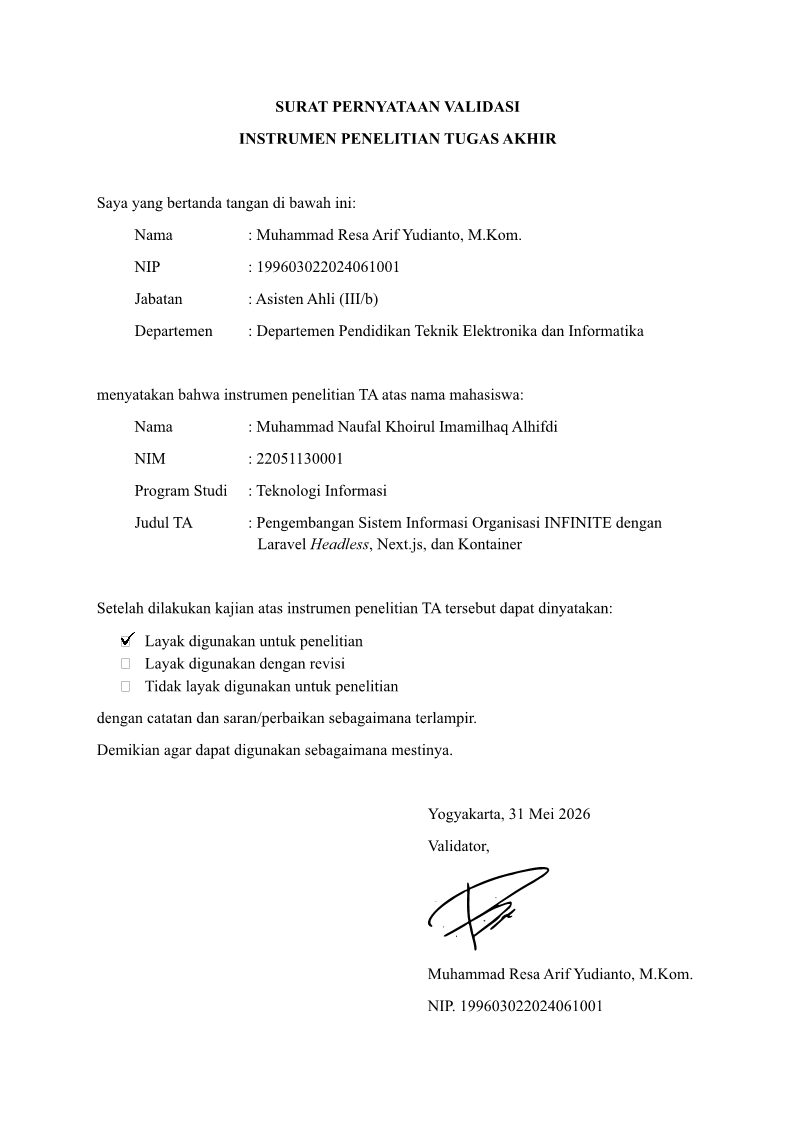
\includegraphics[width=1\textwidth,keepaspectratio]{images/surat-validasi-instrumen.png}
\end{figure}

\newpage

\annex{\textit{Use Case Diagram} Aktor Terautentikasi}
\label{annex:use-case-diagram-authenticated-user}

\noindent
\textit{Use case diagram} dipecah dalam beberapa diagram untuk memudahkan pembacaan, karena diagram keseluruhan akan menjadi terlalu besar. Setiap diagram menampilkan aktor dan fitur sistem yang saling berinteraksi sesuai dengan domain fitur yang ada.

\begin{figure}[H]
      \centering
      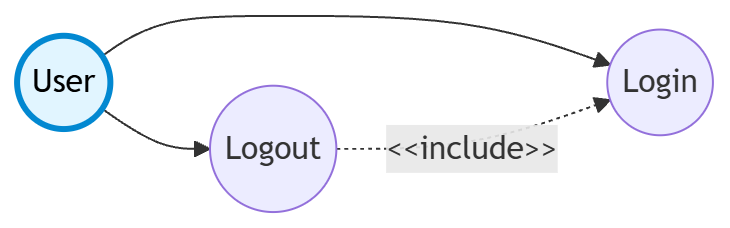
\includegraphics[width=0.45\textwidth,keepaspectratio]{images/umls/use-case-authn-diagram.png}
\end{figure}

\begin{figure}[H]
      \centering
      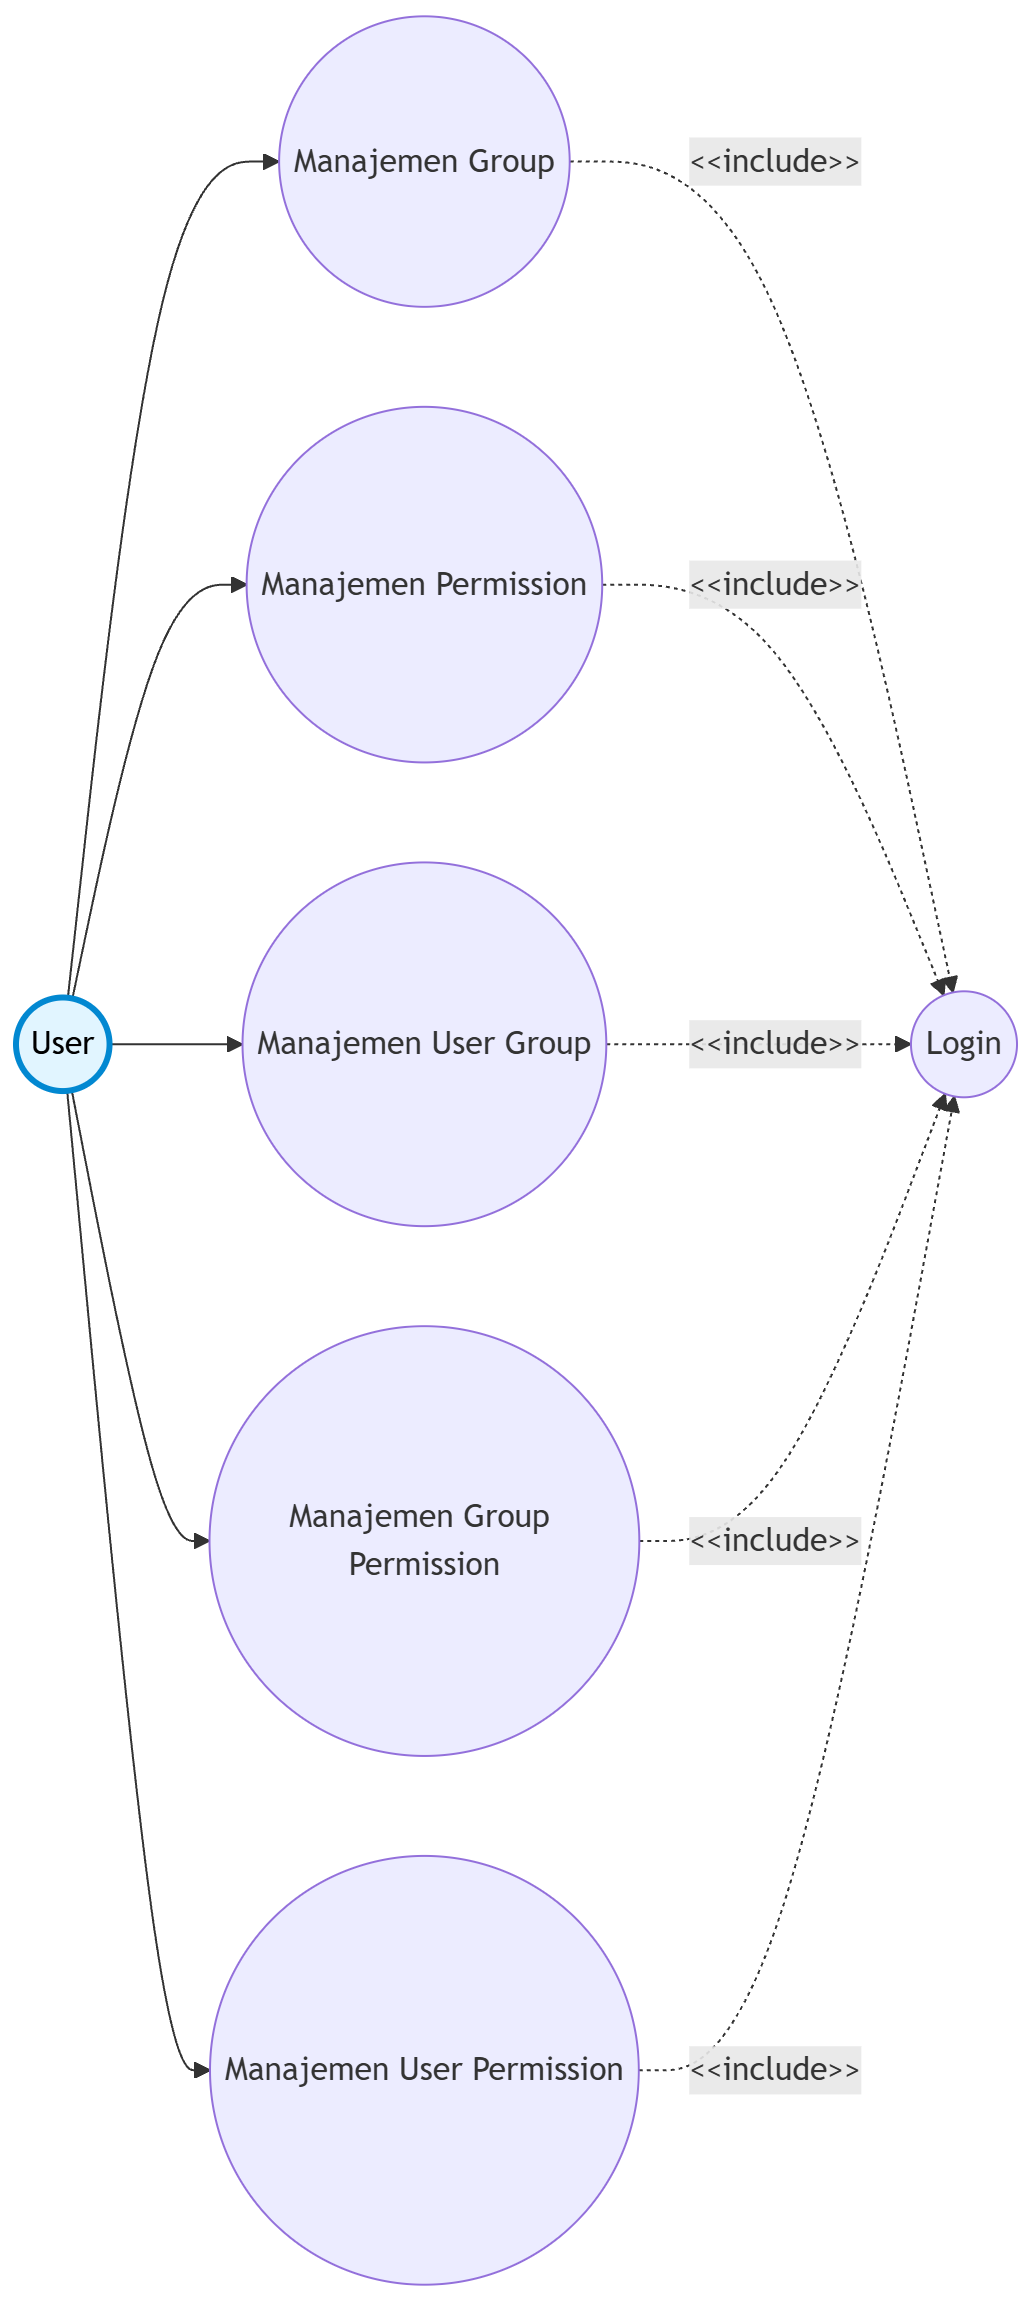
\includegraphics[width=0.55\textwidth,keepaspectratio]{images/umls/use-case-authz-diagram.png}
\end{figure}

\begin{figure}[H]
      \centering
      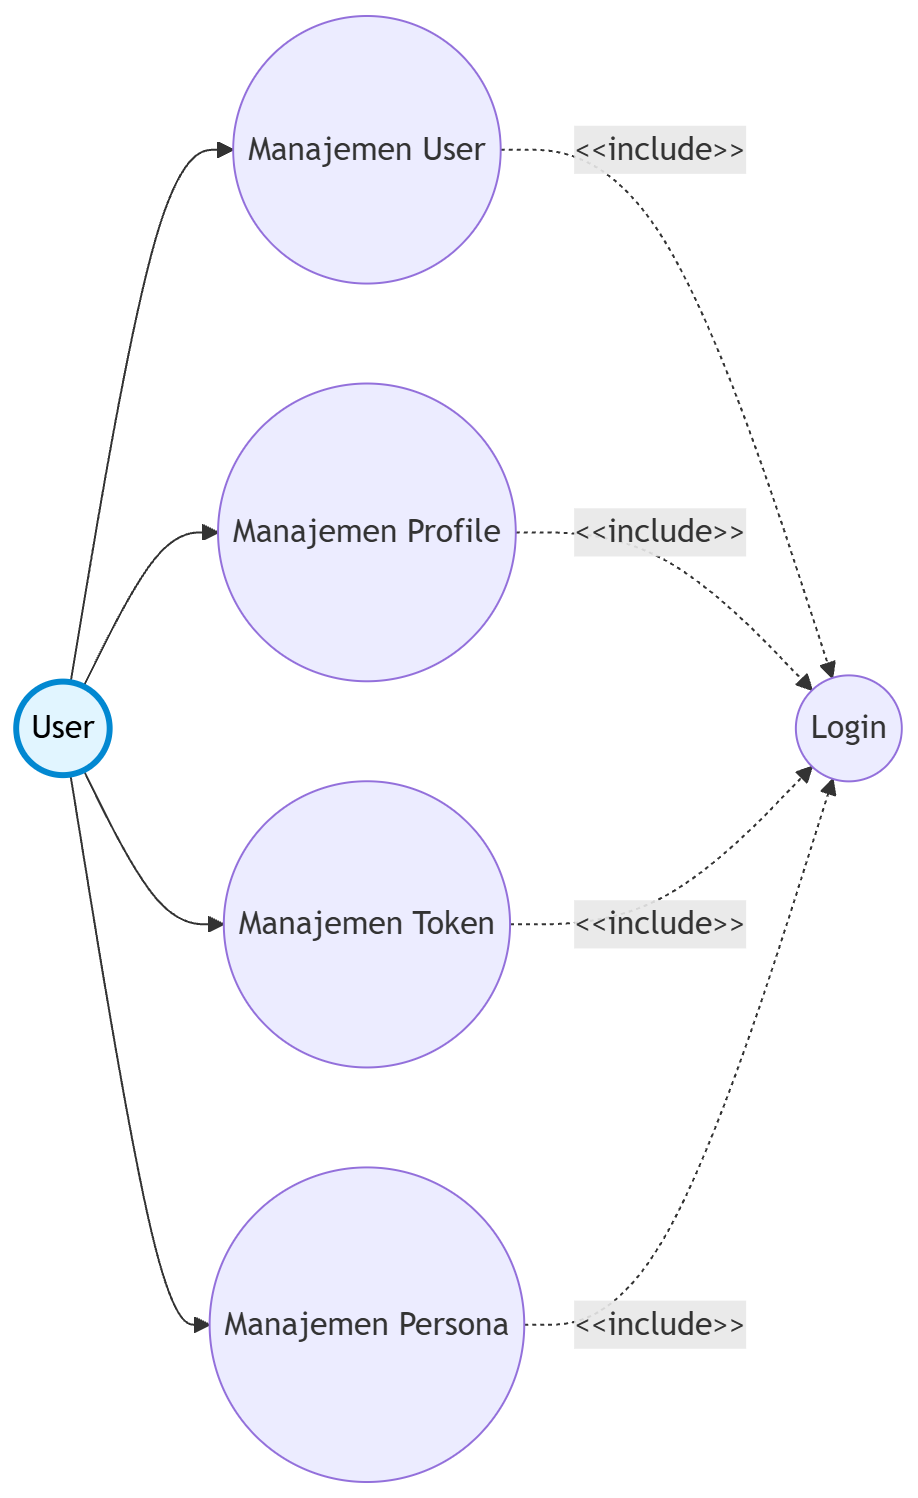
\includegraphics[width=0.5\textwidth,keepaspectratio]{images/umls/use-case-user-diagram.png}
\end{figure}

\begin{figure}[H]
      \centering
      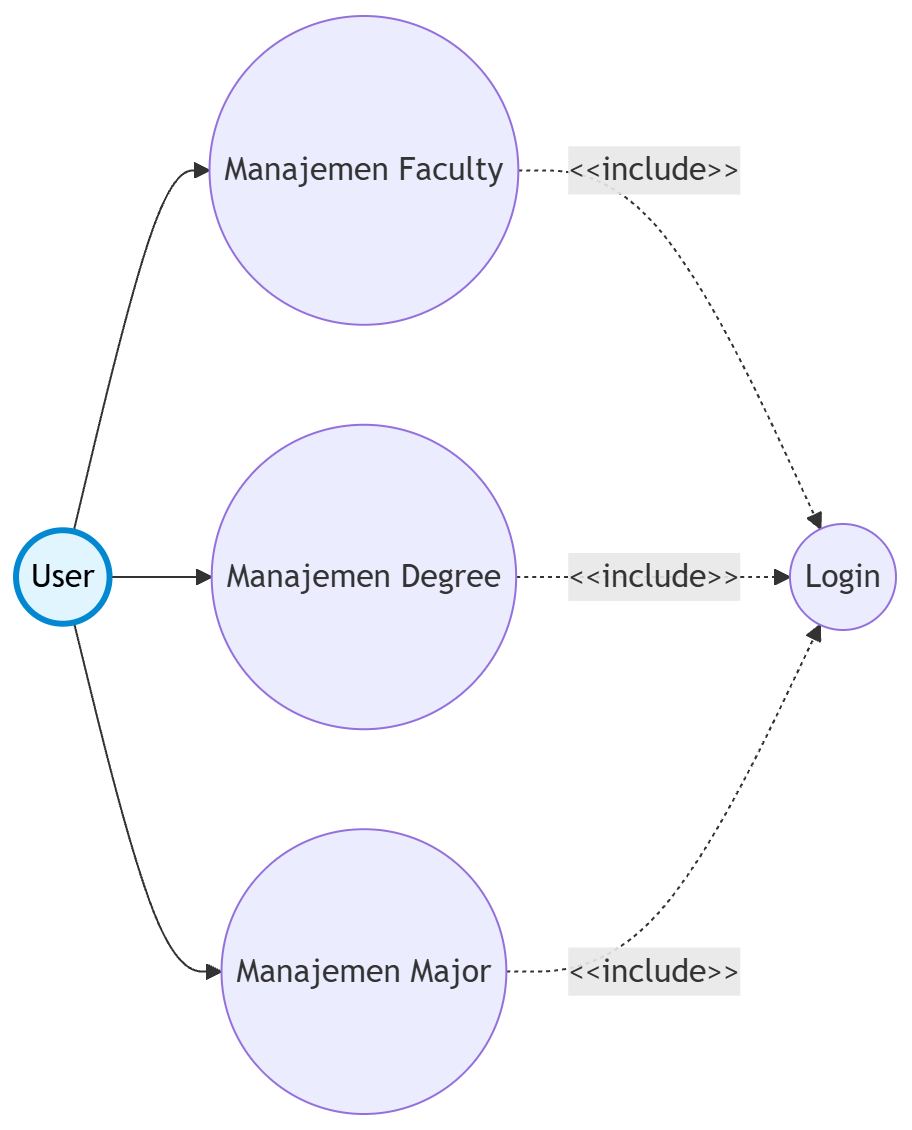
\includegraphics[width=0.5\textwidth,keepaspectratio]{images/umls/use-case-academic-diagram.png}
\end{figure}

\begin{figure}[H]
      \centering
      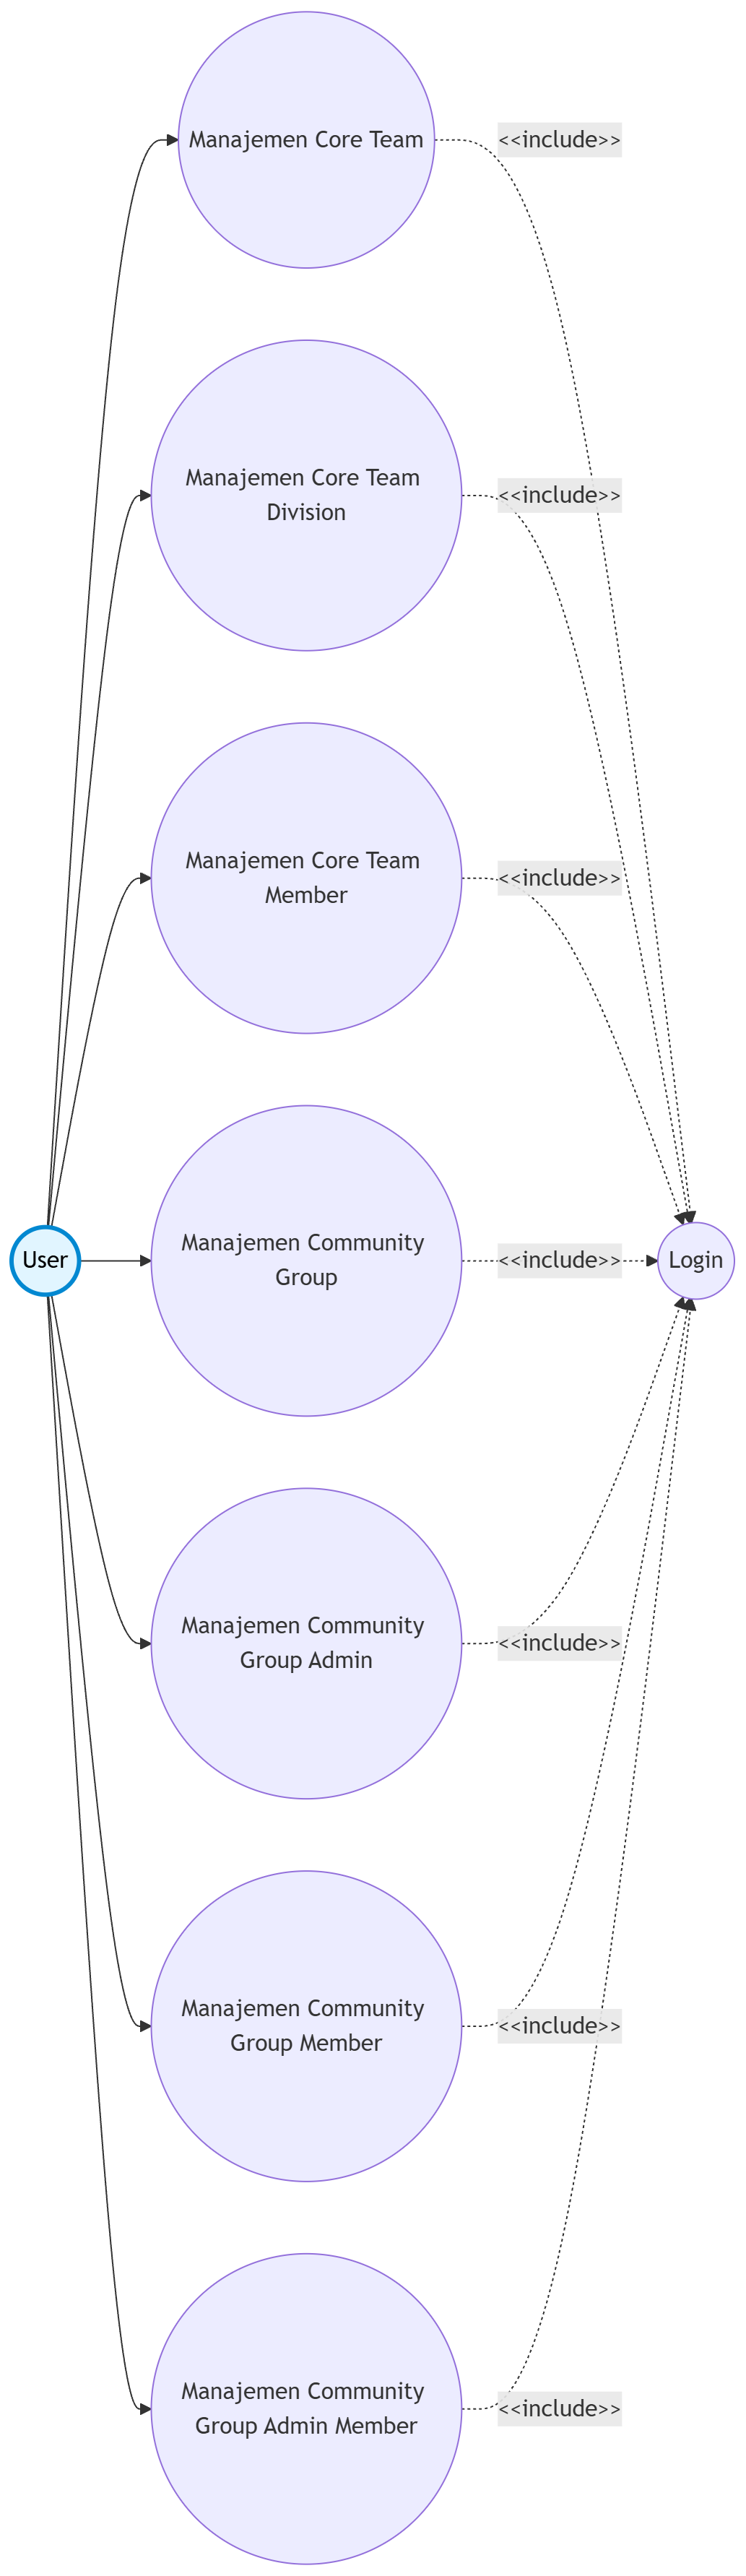
\includegraphics[height=1\textheight,keepaspectratio]{images/umls/use-case-organization-diagram.png}
\end{figure}

\begin{figure}[H]
      \centering
      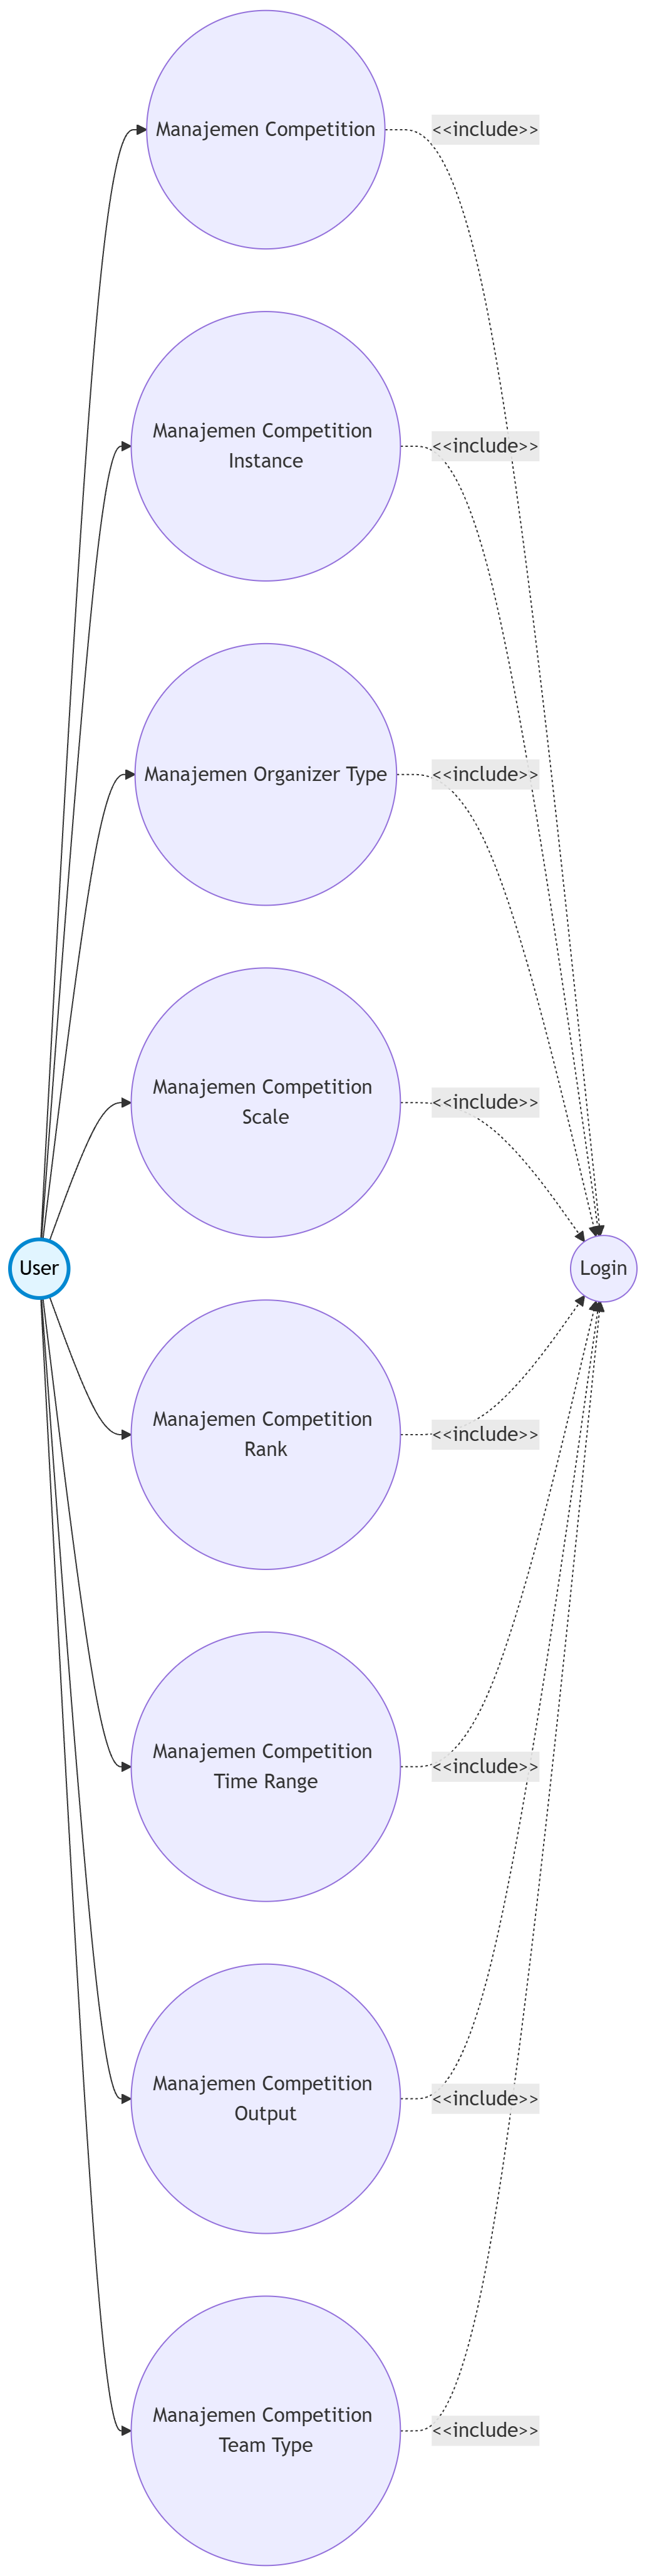
\includegraphics[height=1\textheight,keepaspectratio]{images/umls/use-case-competition-diagram.png}
\end{figure}

\begin{figure}[H]
      \centering
      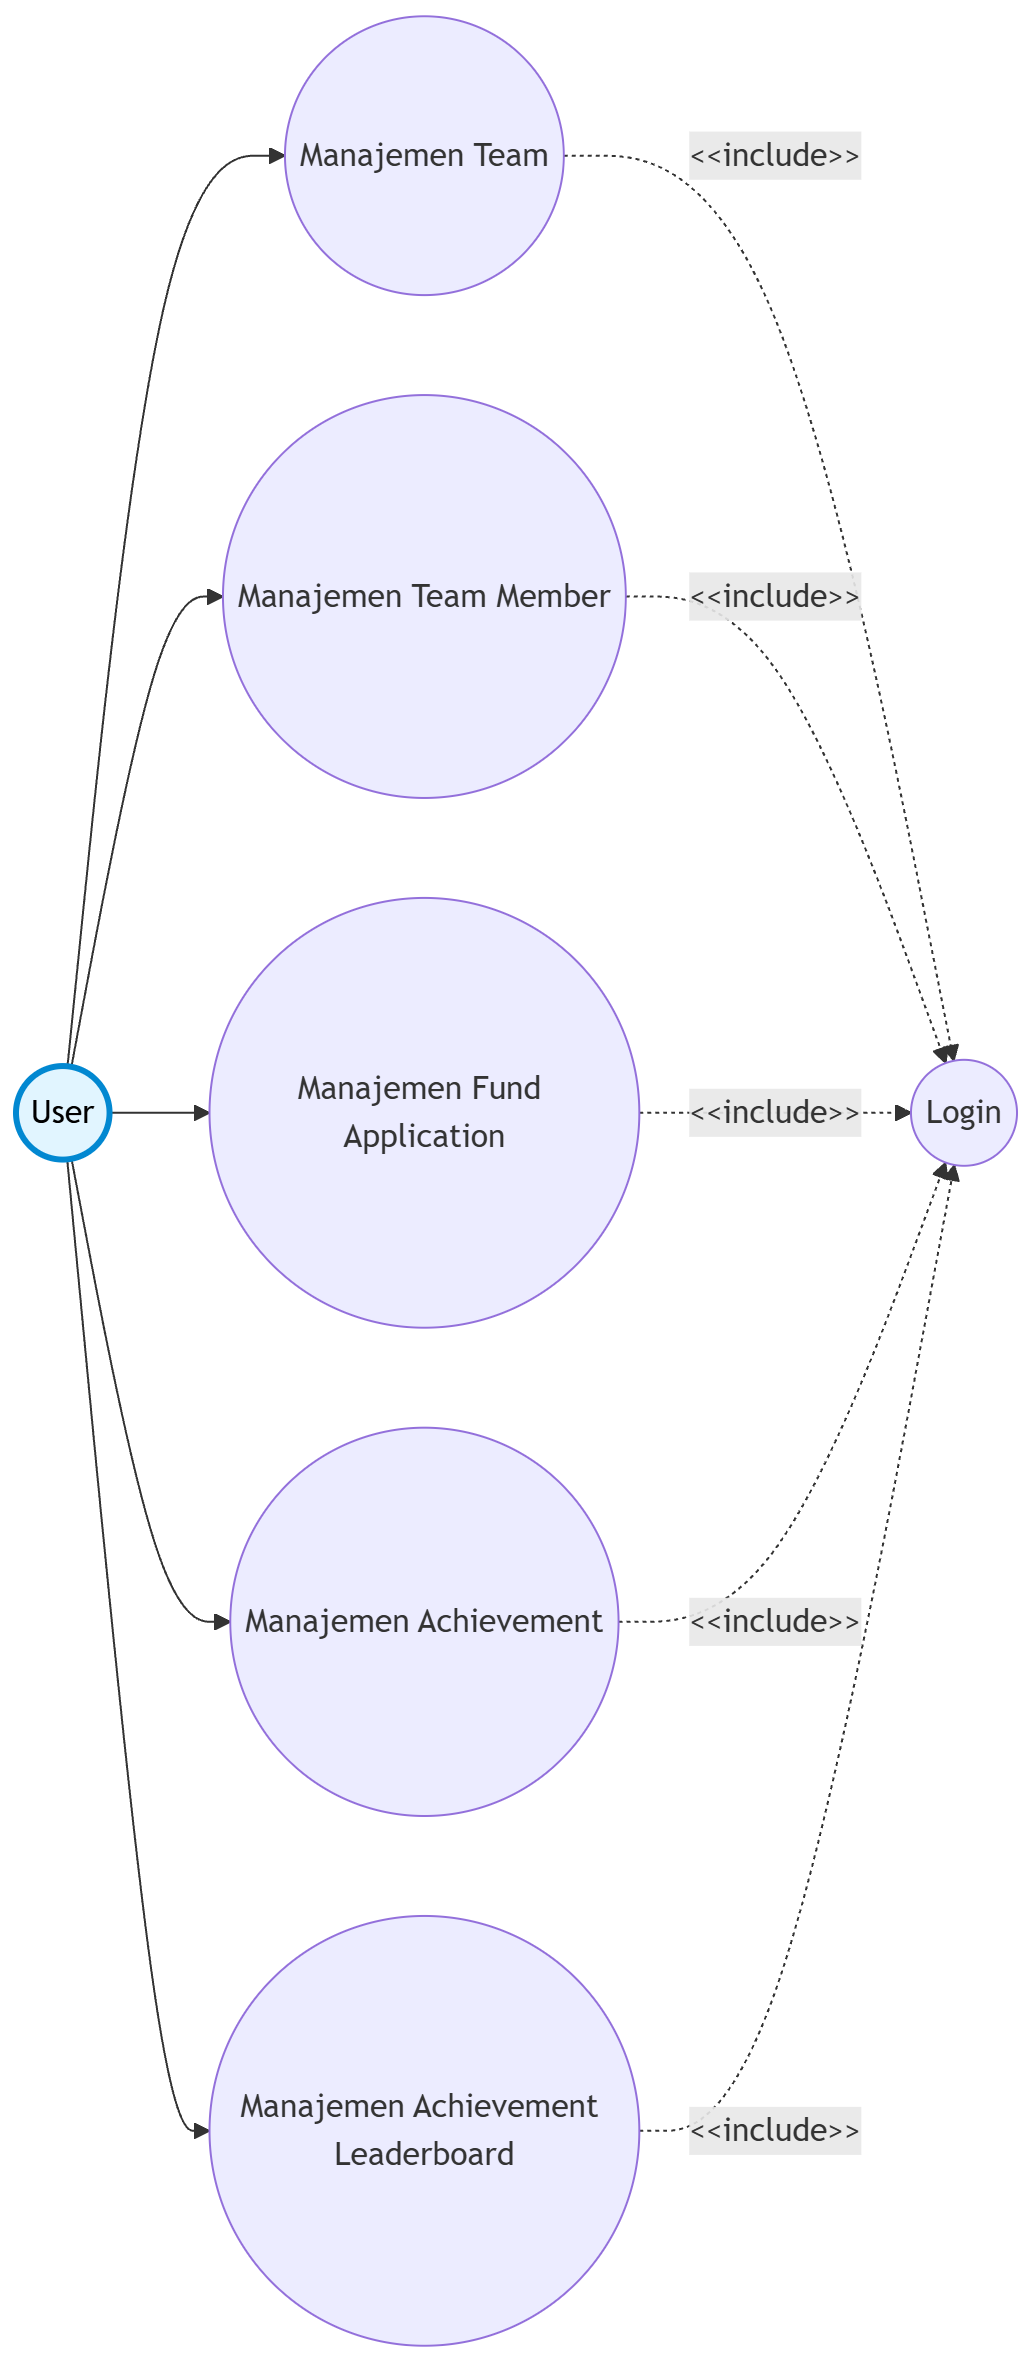
\includegraphics[width=0.6\textwidth,keepaspectratio]{images/umls/use-case-team-achievement-diagram.png}
\end{figure}

\begin{figure}[H]
      \centering
      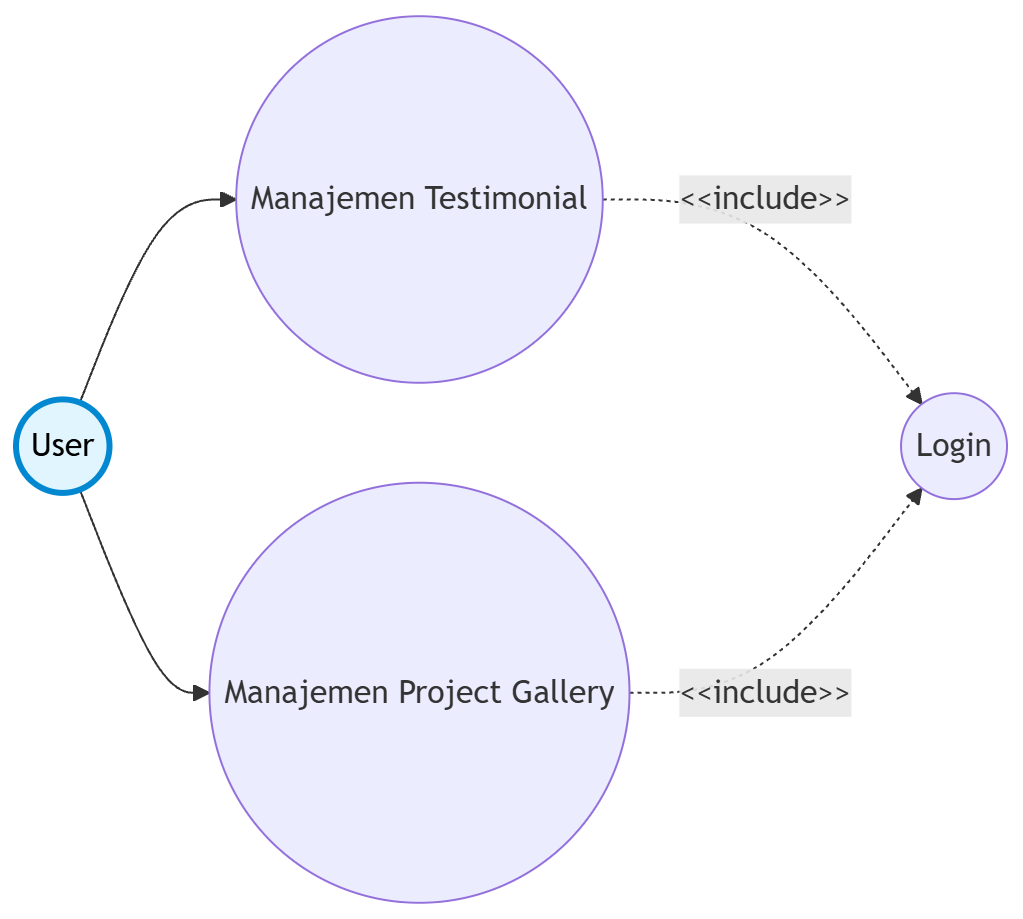
\includegraphics[width=0.6\textwidth,keepaspectratio]{images/umls/use-case-content-diagram.png}
\end{figure}

\begin{figure}[H]
      \centering
      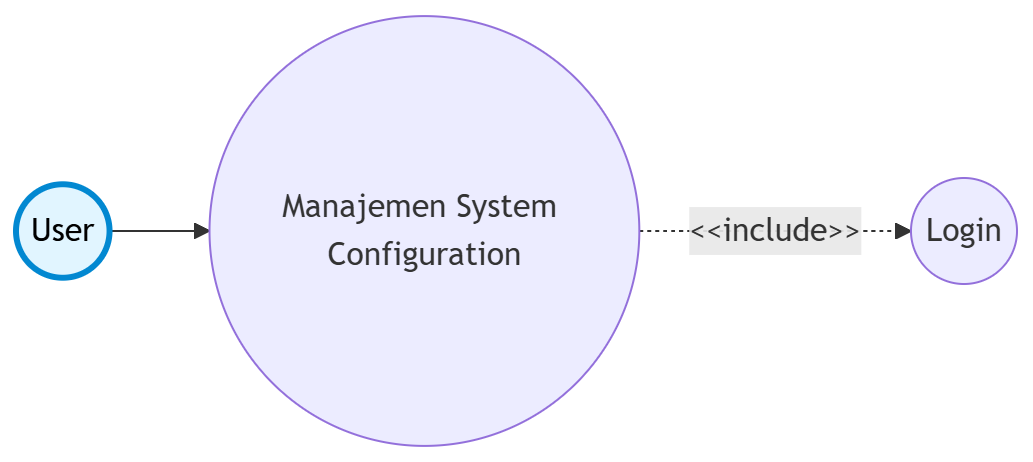
\includegraphics[width=0.6\textwidth,keepaspectratio]{images/umls/use-case-configuration-diagram.png}
\end{figure}

\newpage

\annex{\textit{Use Case Description}}
\label{annex:use-case-description}

\begin{longtable}{|p{0.05\linewidth}|p{0.30\linewidth}|p{0.58\linewidth}|}
      \hline
      \textbf{No} & \textbf{\textit{Use Case}}             & \textbf{Deskripsi}                                                                                    \\
      \hline
      \endfirsthead

      \hline
      \textbf{No} & \textbf{\textit{Use Case}}             & \textbf{Deskripsi}                                                                                    \\
      \hline
      \endhead

      \hline
      \endfoot

      \hline
      \endlastfoot

      1           & Login                                  & Berfungsi untuk masuk ke dalam sistem menggunakan kredensial SSO INFINITE yang valid.                 \\
      \hline
      2           & Logout                                 & Berfungsi untuk keluar dari sistem dan mengakhiri sesi autentikasi pengguna.                          \\
      \hline
      3           & Manajemen Group                        & Berfungsi untuk pengelolaan data grup pengguna untuk pengelompokan hak akses.                         \\
      \hline
      4           & Manajemen Permission                   & Berfungsi untuk pengelolaan data izin akses yang dapat diberikan kepada grup atau pengguna.           \\
      \hline
      5           & Manajemen User Group                   & Berfungsi untuk pengelolaan keanggotaan grup dari setiap pengguna dalam sistem.                       \\
      \hline
      6           & Manajemen Group Permission             & Berfungsi untuk pengelolaan izin akses yang diberikan kepada setiap grup.                             \\
      \hline
      7           & Manajemen User Permission              & Berfungsi untuk pengelolaan izin akses khusus yang diberikan langsung kepada pengguna tertentu.       \\
      \hline
      8           & Manajemen Faculty                      & Berfungsi untuk pengelolaan data fakultas yang tersedia dalam sistem.                                 \\
      \hline
      9           & Manajemen Degree                       & Berfungsi untuk pengelolaan data strata pendidikan (S1, S2, S3, D3, D4).                              \\
      \hline
      10          & Manajemen Major                        & Berfungsi untuk pengelolaan data program studi yang tersedia dalam sistem.                            \\
      \hline
      11          & Manajemen User                         & Berfungsi untuk pengelolaan data anggota organisasi termasuk informasi profil dan status keanggotaan. \\
      \hline
      12          & Manajemen Profile                      & Berfungsi untuk pengelolaan data profil pribadi termasuk informasi kontak dan preferensi.             \\
      \hline
      13          & Manajemen Token                        & Berfungsi untuk pengelolaan token akses API untuk integrasi dengan sistem eksternal.                  \\
      \hline
      14          & Manajemen Persona                      & Berfungsi untuk pengelolaan kategori anggota (persona) untuk klasifikasi dan segmentasi pengguna.     \\
      \hline
      15          & Manajemen Core Team                    & Berfungsi untuk pengelolaan data kepengurusan inti organisasi untuk periode tertentu.                 \\
      \hline
      16          & Manajemen Core Team Division           & Berfungsi untuk pengelolaan divisi atau departemen dalam struktur kepengurusan inti.                  \\
      \hline
      17          & Manajemen Core Team Member             & Berfungsi untuk pengelolaan anggota kepengurusan inti termasuk penempatan divisi dan foto.            \\
      \hline
      18          & Manajemen Community Group              & Berfungsi untuk pengelolaan kelompok komunitas yang merupakan subdivisi dari organisasi utama.        \\
      \hline
      19          & Manajemen Community Group Admin        & Berfungsi untuk pengelolaan administrator untuk setiap kelompok komunitas.                            \\
      \hline
      20          & Manajemen Community Group Member       & Berfungsi untuk pengelolaan keanggotaan dalam setiap kelompok komunitas.                              \\
      \hline
      21          & Manajemen Community Group Admin Member & Berfungsi untuk pengelolaan anggota administrator dalam setiap kelompok komunitas.                    \\
      \hline
      22          & Manajemen Competition                  & Berfungsi untuk pengelolaan data seri kompetisi yang diselenggarakan oleh organisasi.                 \\
      \hline
      23          & Manajemen Competition Instance         & Berfungsi untuk pengelolaan edisi pelaksanaan kompetisi dari suatu seri kompetisi.                    \\
      \hline
      24          & Manajemen Organizer Type               & Berfungsi untuk pengelolaan jenis penyelenggara kompetisi (internal, eksternal, kolaborasi).          \\
      \hline
      25          & Manajemen Competition Scale            & Berfungsi untuk pengelolaan skala kompetisi (lokal, regional, nasional, internasional).               \\
      \hline
      26          & Manajemen Competition Rank             & Berfungsi untuk pengelolaan peringkat atau pencapaian dalam kompetisi.                                \\
      \hline
      27          & Manajemen Competition Time Range       & Berfungsi untuk pengelolaan rentang waktu pelaksanaan kompetisi.                                      \\
      \hline
      28          & Manajemen Competition Output           & Berfungsi untuk pengelolaan luaran atau hasil yang dihasilkan dari kompetisi.                         \\
      \hline
      29          & Manajemen Competition Team Type        & Berfungsi untuk pengelolaan jenis tim yang dapat berpartisipasi dalam kompetisi (individu, tim).      \\
      \hline
      30          & Manajemen Team                         & Berfungsi untuk pengelolaan data tim yang terdaftar dalam sistem untuk keperluan kompetisi.           \\
      \hline
      31          & Manajemen Team Member                  & Berfungsi untuk pengelolaan keanggotaan tim termasuk peran dan kontribusi anggota.                    \\
      \hline
      32          & Manajemen Achievement                  & Berfungsi untuk pengelolaan data prestasi anggota beserta status persetujuan.                         \\
      \hline
      33          & Manajemen Achievement Leaderboard      & Berfungsi untuk pengelolaan papan peringkat prestasi untuk menampilkan pencapaian terbaik.            \\
      \hline
      34          & Manajemen Fund Application             & Berfungsi untuk pengelolaan pengajuan dana dari anggota beserta status persetujuan.                   \\
      \hline
      35          & Manajemen Testimonial                  & Berfungsi untuk pengelolaan testimoni dari anggota tentang pengalaman mereka dengan organisasi.       \\
      \hline
      36          & Manajemen Project Gallery              & Berfungsi untuk pengelolaan galeri proyek yang menampilkan hasil karya anggota organisasi.            \\
      \hline
      37          & Manajemen System Configuration         & Berfungsi untuk pengelolaan konfigurasi sistem termasuk pengaturan daftar ulang keanggotaan.          \\
      \hline
      38          & Lihat Competition                      & Berfungsi untuk menampilkan daftar seri kompetisi yang tersedia tanpa perlu autentikasi.              \\
      \hline
      39          & Lihat Competition Instance             & Berfungsi untuk menampilkan detail edisi pelaksanaan kompetisi tanpa perlu autentikasi.               \\
      \hline
      40          & Lihat Core Team                        & Berfungsi untuk menampilkan struktur kepengurusan inti organisasi tanpa perlu autentikasi.            \\
      \hline
      41          & Lihat Community Group                  & Berfungsi untuk menampilkan daftar kelompok komunitas tanpa perlu autentikasi.                        \\
      \hline
      42          & Lihat Achievement                      & Berfungsi untuk menampilkan daftar prestasi anggota tanpa perlu autentikasi.                          \\
      \hline
      43          & Lihat Achievement Leaderboard          & Berfungsi untuk menampilkan papan peringkat prestasi tanpa perlu autentikasi.                         \\
      \hline
      44          & Lihat Testimonial                      & Berfungsi untuk menampilkan testimoni anggota tanpa perlu autentikasi.                                \\
      \hline
      45          & Lihat Project Gallery                  & Berfungsi untuk menampilkan galeri proyek tanpa perlu autentikasi.                                    \\
      \hline
\end{longtable}

\newpage

\annex{Kode Program Migrasi Tabel \texttt{users}}
\label{annex:code-migration-file}

\lstinputlisting[language=PHP, label=lst:migration-file]{code/database/migration.php}

\annex{Kode Program \textit{seeder} untuk Data \texttt{groups}}
\label{annex:code-seeder-file}

\lstinputlisting[language=PHP , label=lst:seeder-file]{code/database/seeder.php}

\annex{Kode Program \textit{Model} \texttt{User}}
\label{annex:code-model-file}

\lstinputlisting[language=PHP, label=lst:model-file]{code/backend/model.php}

\annex{Kode Program \textit{Custom Resource}}
\label{annex:code-base-resource-file}

\lstinputlisting[language=PHP, label=lst:base-resource-file]{code/backend/base-resource.php}

\annex{Kode Program \textit{Custom Resource Collection}}
\label{annex:code-base-collection-file}

\lstinputlisting[language=PHP, label=lst:base-collection-file]{code/backend/base-collection.php}

\annex{Kode Program \textit{Resource} untuk \textit{Model} \texttt{User}}
\label{annex:code-user-resource-file}

\lstinputlisting[language=PHP, label=lst:user-resource-file]{code/backend/user-resource.php}

\annex{Kode Program \textit{Resource Collection} untuk \textit{Model} \texttt{User}}
\label{annex:code-user-collection-file}

\lstinputlisting[language=PHP, label=lst:user-collection-file]{code/backend/user-collection.php}

\annex{Kode Program \textit{Controller} \texttt{UserController}}
\label{annex:code-user-controller-file}

\lstinputlisting[language=PHP, label=lst:user-controller-file]{code/backend/user-controller.php}

\annex{Kode Program \textit{Service} \texttt{OidcService}}
\label{annex:code-oidc-service-file}

\lstinputlisting[language=PHP, label=lst:oidc-service-file]{code/backend/oidc-service.php}

\annex{Kode Program \textit{Service} \texttt{SsoService}}
\label{annex:code-sso-service-file}

\lstinputlisting[language=PHP, label=lst:sso-service-file]{code/backend/sso-service.php}

\annex{Kode Program \textit{Repository} \texttt{StorageRepository}}
\label{annex:code-storage-repository-file}

\lstinputlisting[language=PHP, label=lst:storage-repository-file]{code/backend/storage-repository.php}

\annex{Kode Program \textit{Guard} \texttt{OidcTokenGuard}}
\label{annex:code-oidc-token-guard-file}

\lstinputlisting[language=PHP, label=lst:oidc-token-guard-file]{code/backend/oidc-token-guard.php}

\annex{Kode Program \textit{Guard} \texttt{OidcHeadersGuard}}
\label{annex:code-oidc-headers-guard-file}

\lstinputlisting[language=PHP, label=lst:oidc-headers-guard-file]{code/backend/oidc-headers-guard.php}

\annex{Kode Program \textit{Job} \texttt{SyncAchievementLeaderboards}}
\label{annex:code-sync-achievement-leaderboard-job-file}

\lstinputlisting[language=PHP, label=lst:sync-achievement-leaderboard-job-file]{code/backend/sync-achievement-leaderboard-job.php}

\annex{Kode Program \textit{Cast} \texttt{Blob}}
\label{annex:code-blob-cast-file}

\lstinputlisting[language=PHP, label=lst:blob-cast-file]{code/backend/blob-cast.php}

\annex{Kode Program Entitas \texttt{User}}
\label{annex:code-user-entity-file}

\lstinputlisting[language=TypeScript, label=lst:user-entity-file]{code/frontend/user-entity.ts}

\annex{Kode Program Antarmuka Repositori \texttt{UserRepository}}
\label{annex:code-user-repository-file}

\lstinputlisting[language=TypeScript, label=lst:user-repository-file]{code/frontend/user-repository.ts}

\annex{Kode Program Kelas Kesalahan \texttt{HttpError}}
\label{annex:code-http-error-file}

\lstinputlisting[language=TypeScript, label=lst:http-error-file]{code/frontend/http-error.ts}

\annex{Kode Program \textit{Use Case} \texttt{GetUsers}}
\label{annex:code-get-users-usecase-file}

\lstinputlisting[language=TypeScript, label=lst:get-users-usecase-file]{code/frontend/get-users-usecase.ts}

\annex{Kode Program \textit{Data Source} \texttt{InfinityApiDataSource}}
\label{annex:code-infinity-api-datasource-file}

\lstinputlisting[language=TypeScript, label=lst:infinity-api-datasource-file]{code/frontend/infinity-api-datasource.ts}

\annex{Kode Program DTO \texttt{UserDto}}
\label{annex:code-user-dto-file}

\lstinputlisting[language=TypeScript, label=lst:user-dto-file]{code/frontend/user-dto.ts}

\annex{Kode Program Implementasi Repositori \texttt{UserRepositoryImpl}}
\label{annex:code-user-repository-impl-file}

\lstinputlisting[language=TypeScript, label=lst:user-repository-impl-file]{code/frontend/user-repository-impl.ts}

\annex{Kode Program \textit{Dockerfile} \textit{Backend}}
\label{annex:code-backend-dockerfile-file}

\lstinputlisting[language=Dockerfile, label=lst:backend-dockerfile]{code/backend/Dockerfile}

\annex{Kode Program \textit{Dockerfile} \textit{Frontend}}
\label{annex:code-frontend-dockerfile-file}

\lstinputlisting[language=Dockerfile, label=lst:frontend-dockerfile]{code/frontend/Dockerfile}

\annex{Kode Program \textit{Pipeline} Rilis \textit{Backend}}
\label{annex:code-backend-pipeline-file}

\lstinputlisting[label=lst:backend-pipeline-file]{code/backend/release.yml}

\annex{Kode Program \textit{Pipeline} Rilis \textit{Frontend}}
\label{annex:code-frontend-pipeline-file}

\lstinputlisting[label=lst:frontend-pipeline-file]{code/frontend/release.yml}

\annex{\textit{Deployment} dengan ArgoCD}
\label{annex:deployment-argocd}

\begin{figure}[H]
      \centering
      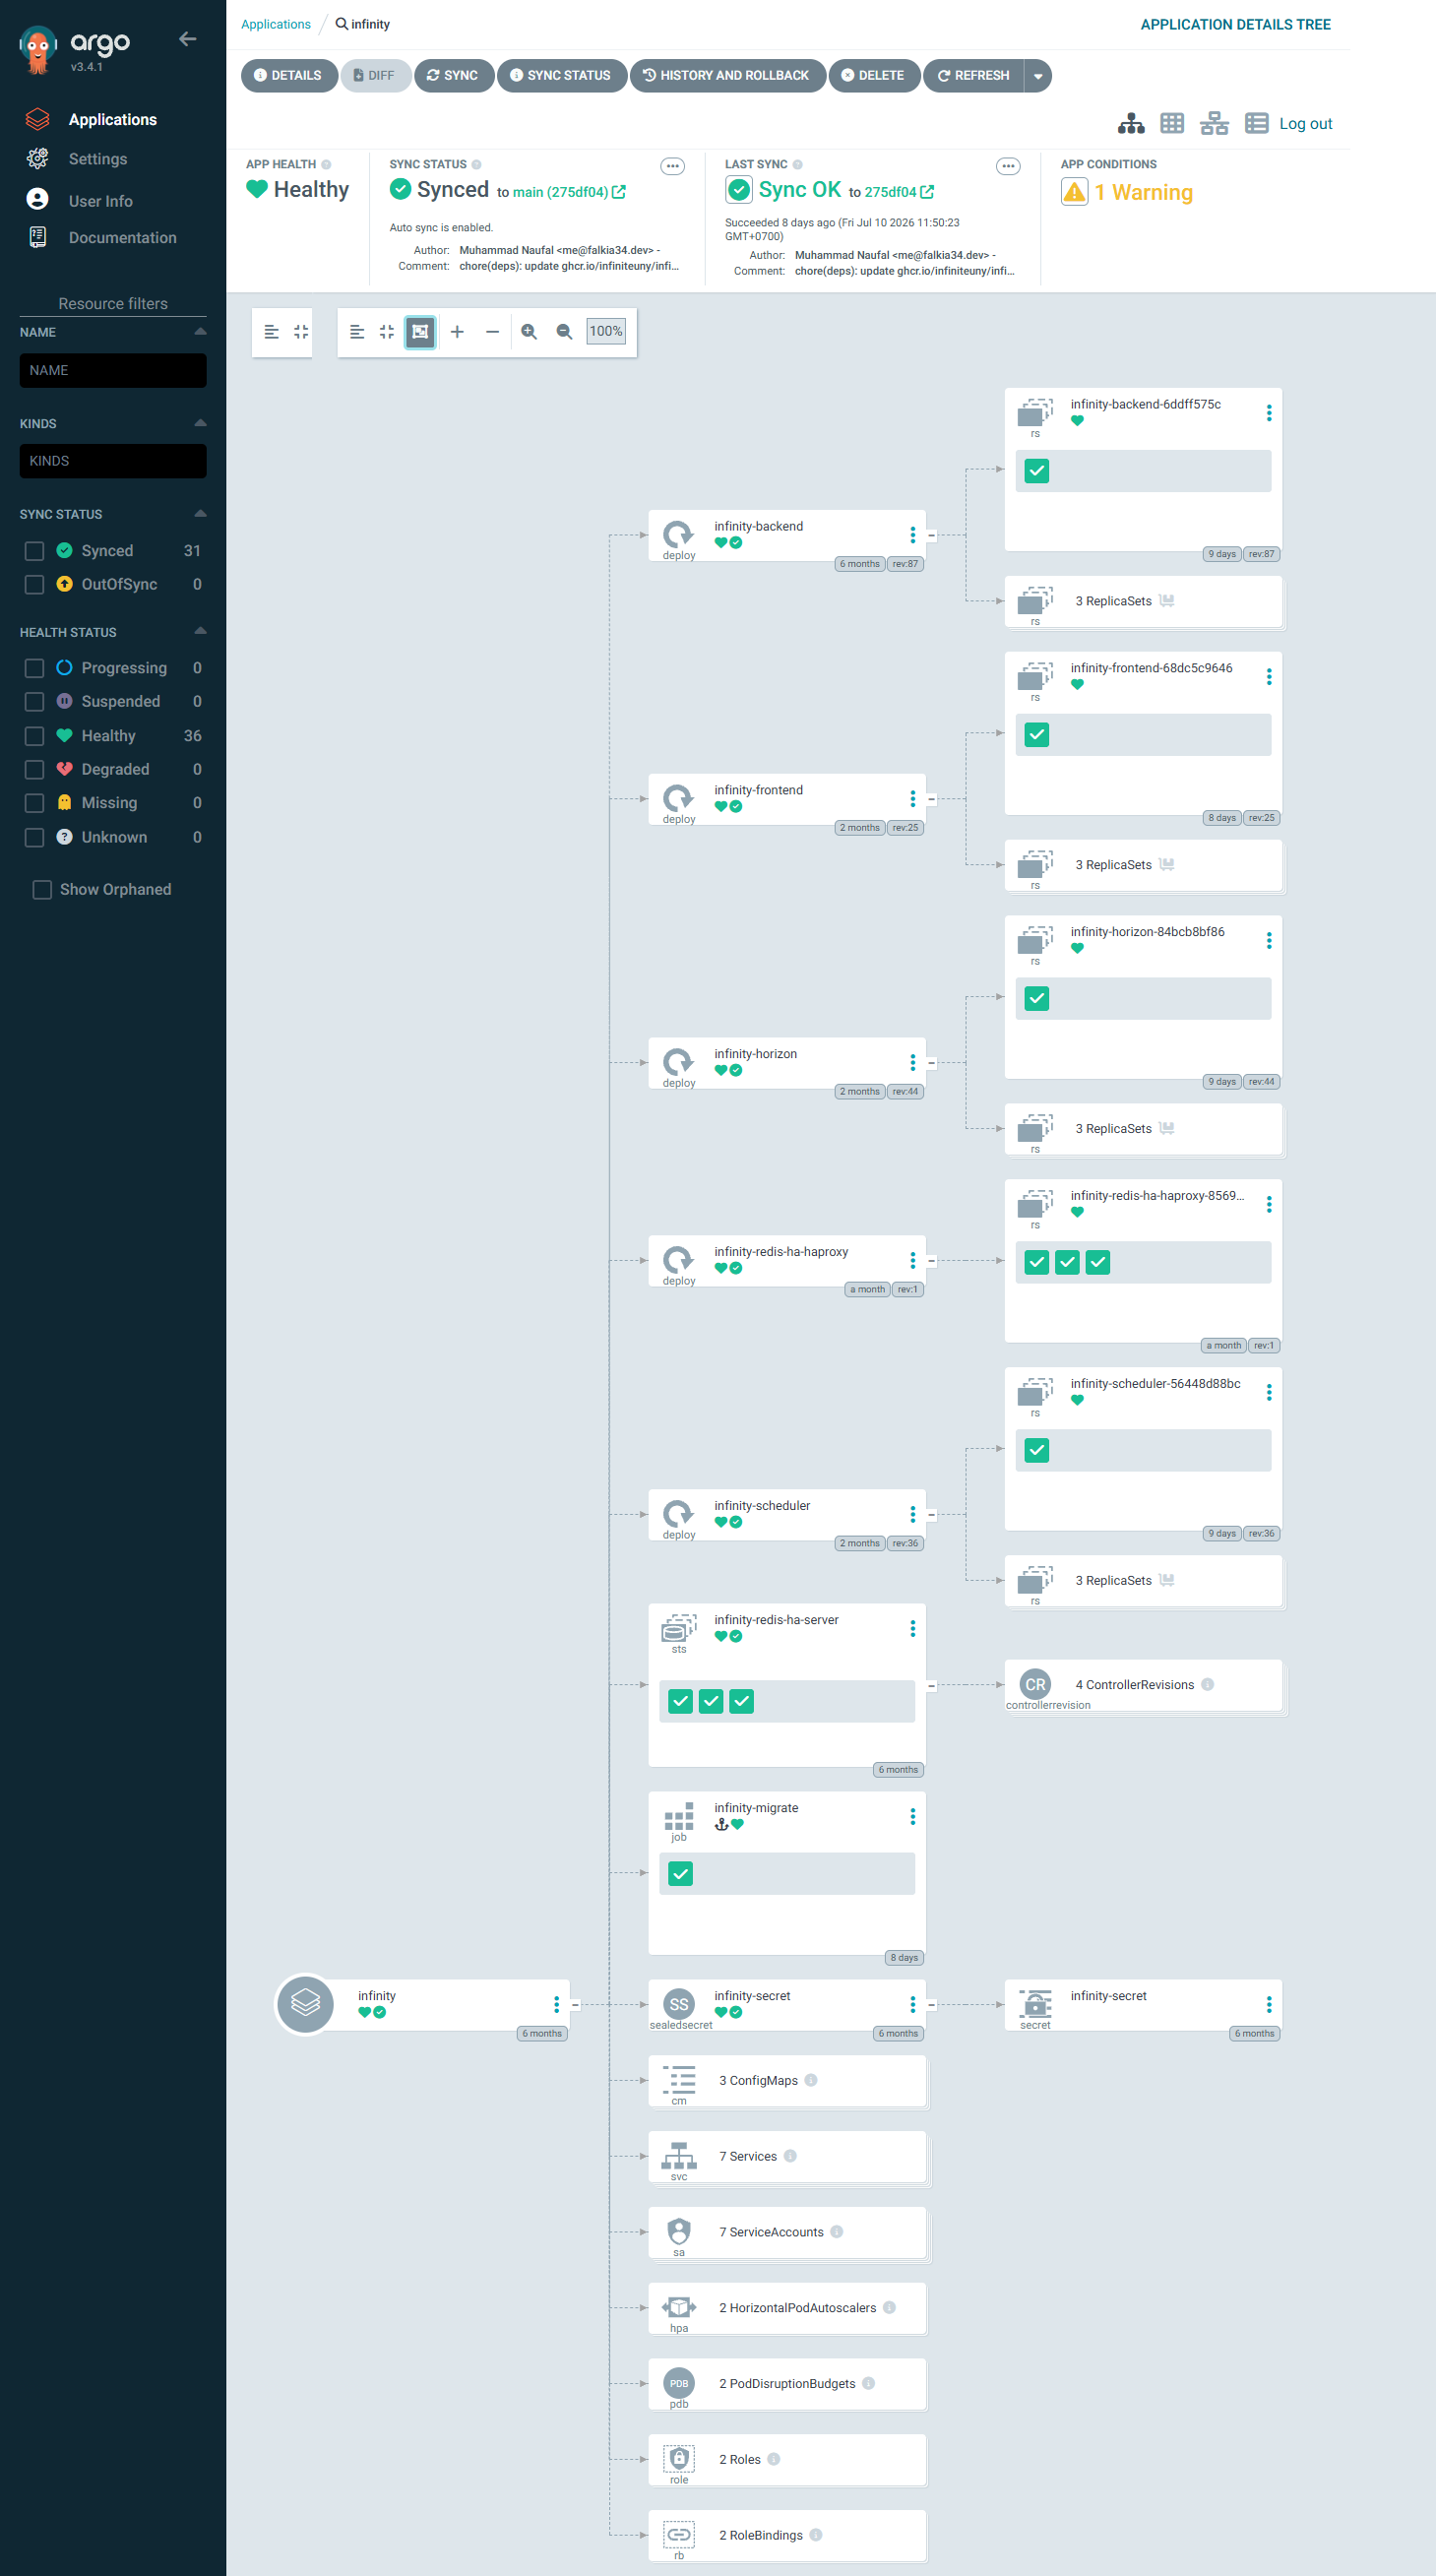
\includegraphics[height=0.94\textheight,keepaspectratio]{images/deployment-argocd.png}
\end{figure}

\parbox[c][\textheight]{\textwidth}{
      \annex{Arsitektur \textit{Deployment} di Kubernetes}
      \label{annex:deployment-architecture-diagram}

      \begin{figure}[H]
            \centering
            \vspace{-1.2cm}
            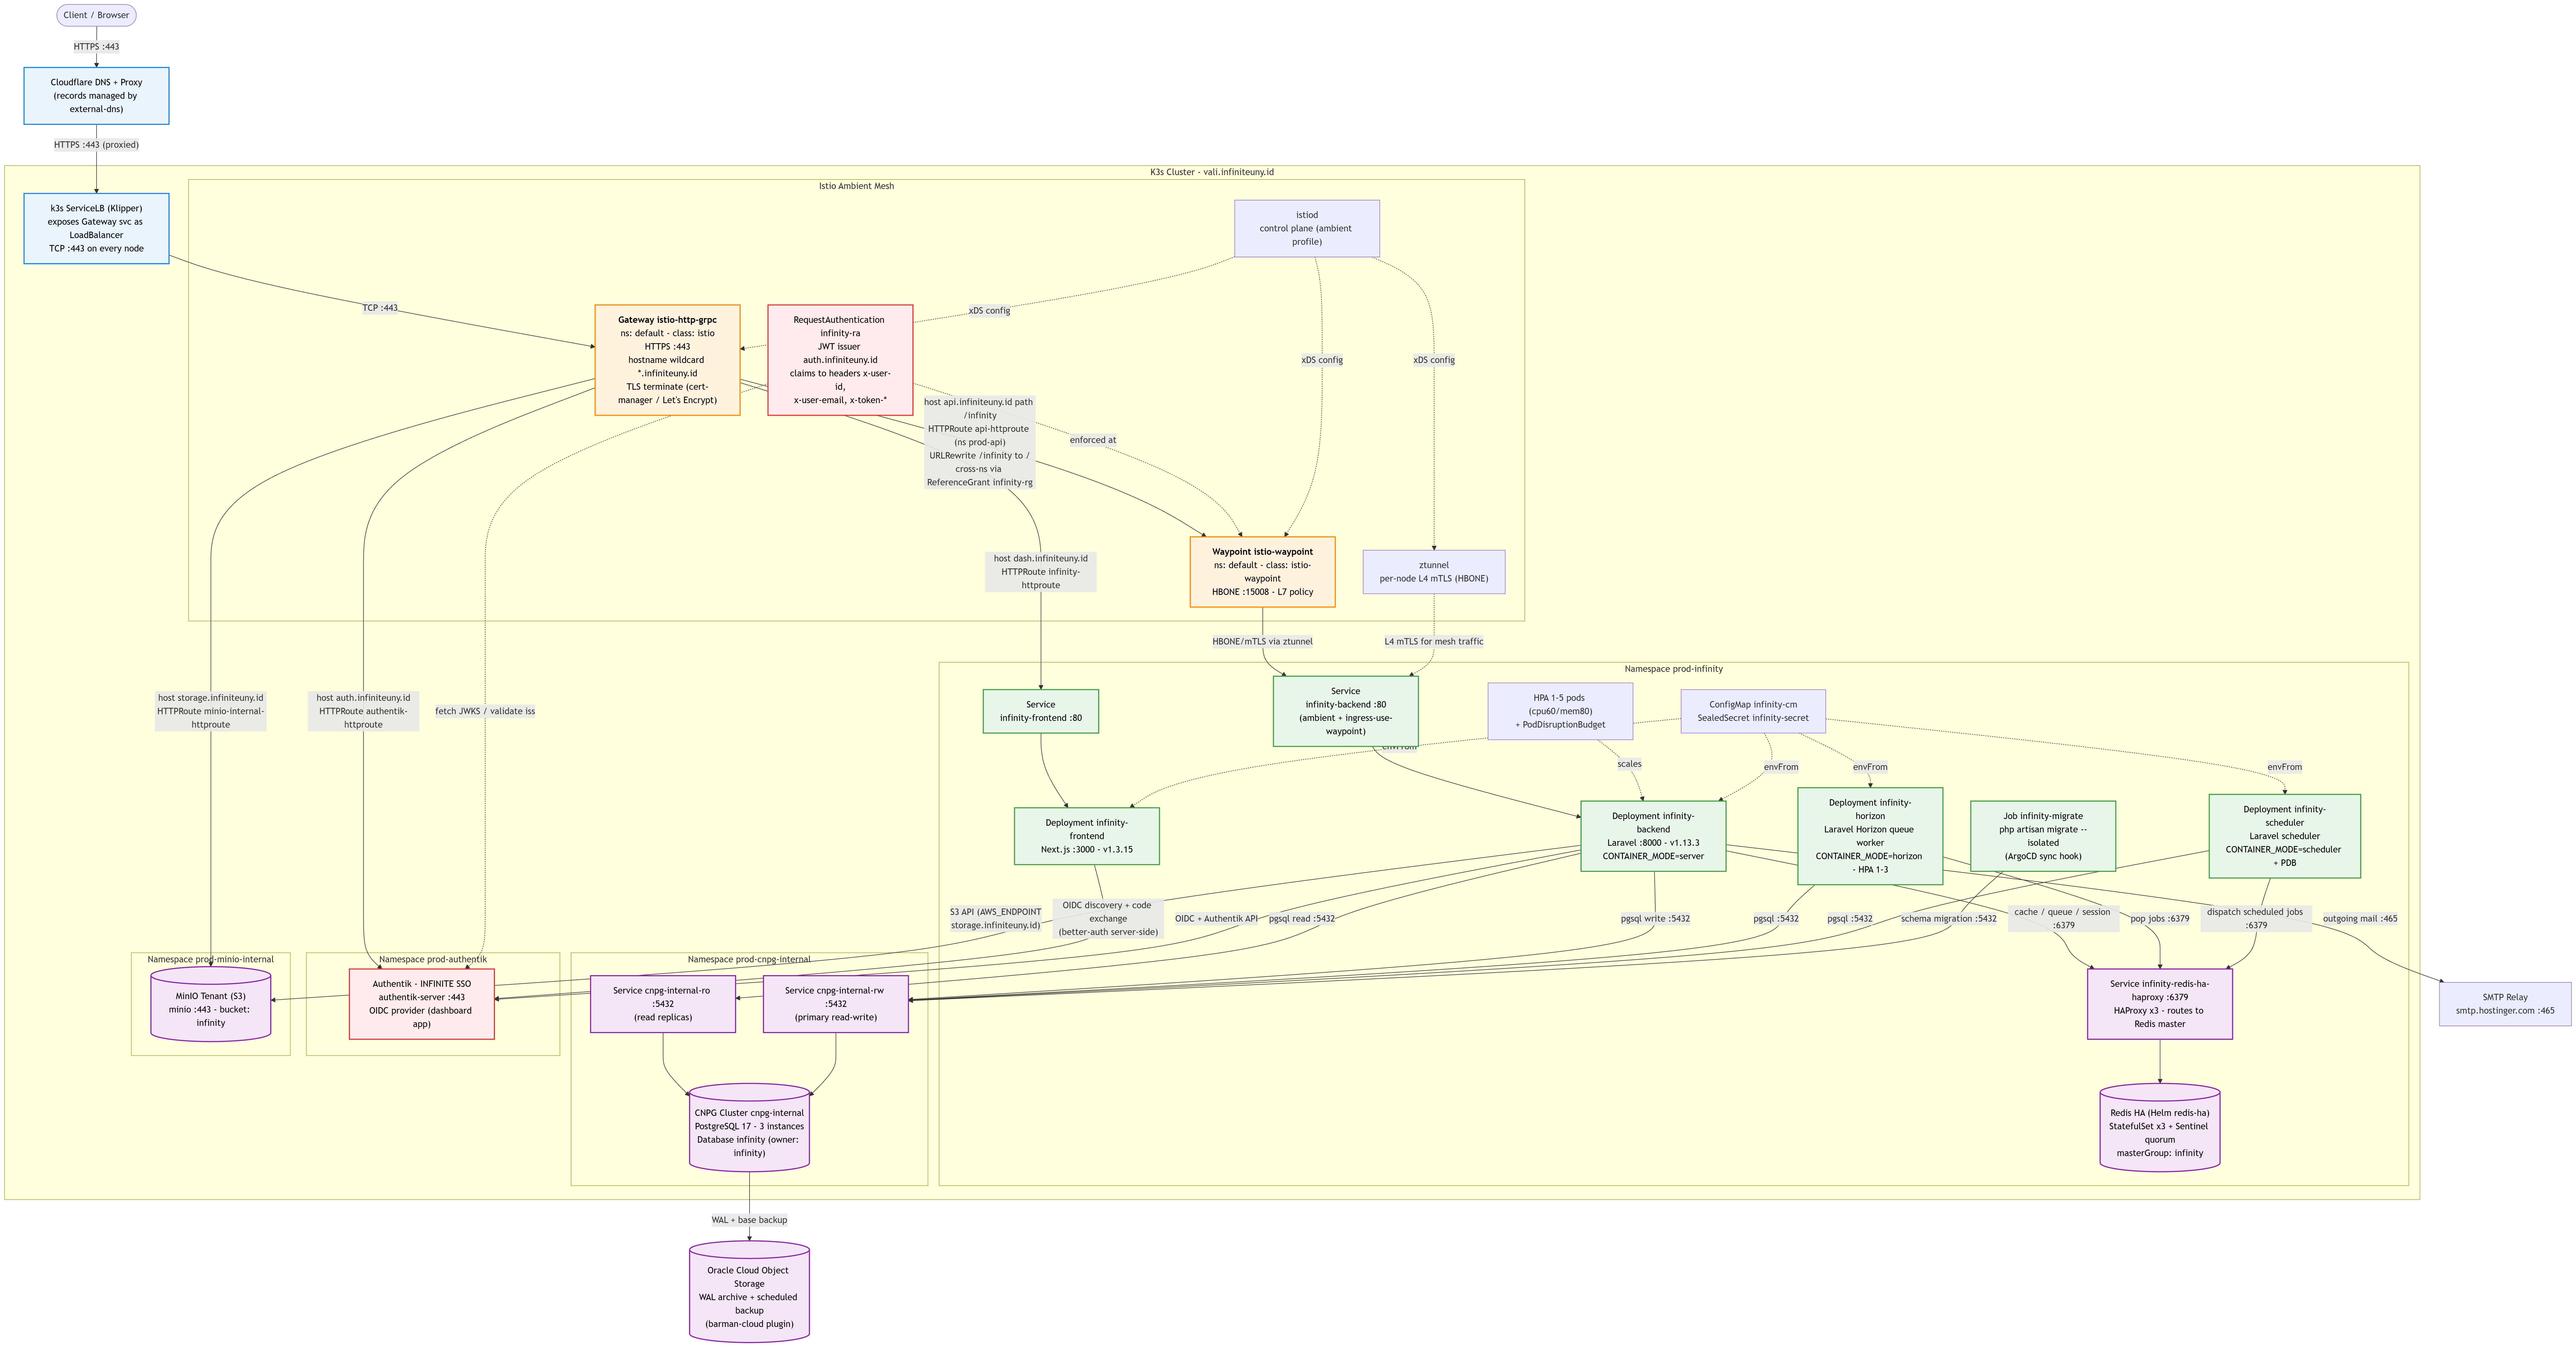
\includegraphics[width=1.07\textheight,angle=90,keepaspectratio]{images/umls/deployment-architecture-diagram.png}
      \end{figure}
}

\newpage

\annex{Hasil Pengujian \textit{Functional Suitability} dan \textit{Interaction Capability}}
\label{annex:functional-suitability-interaction-capability}

\noindent Penguji 1

\begin{figure}[H]
      \centering
      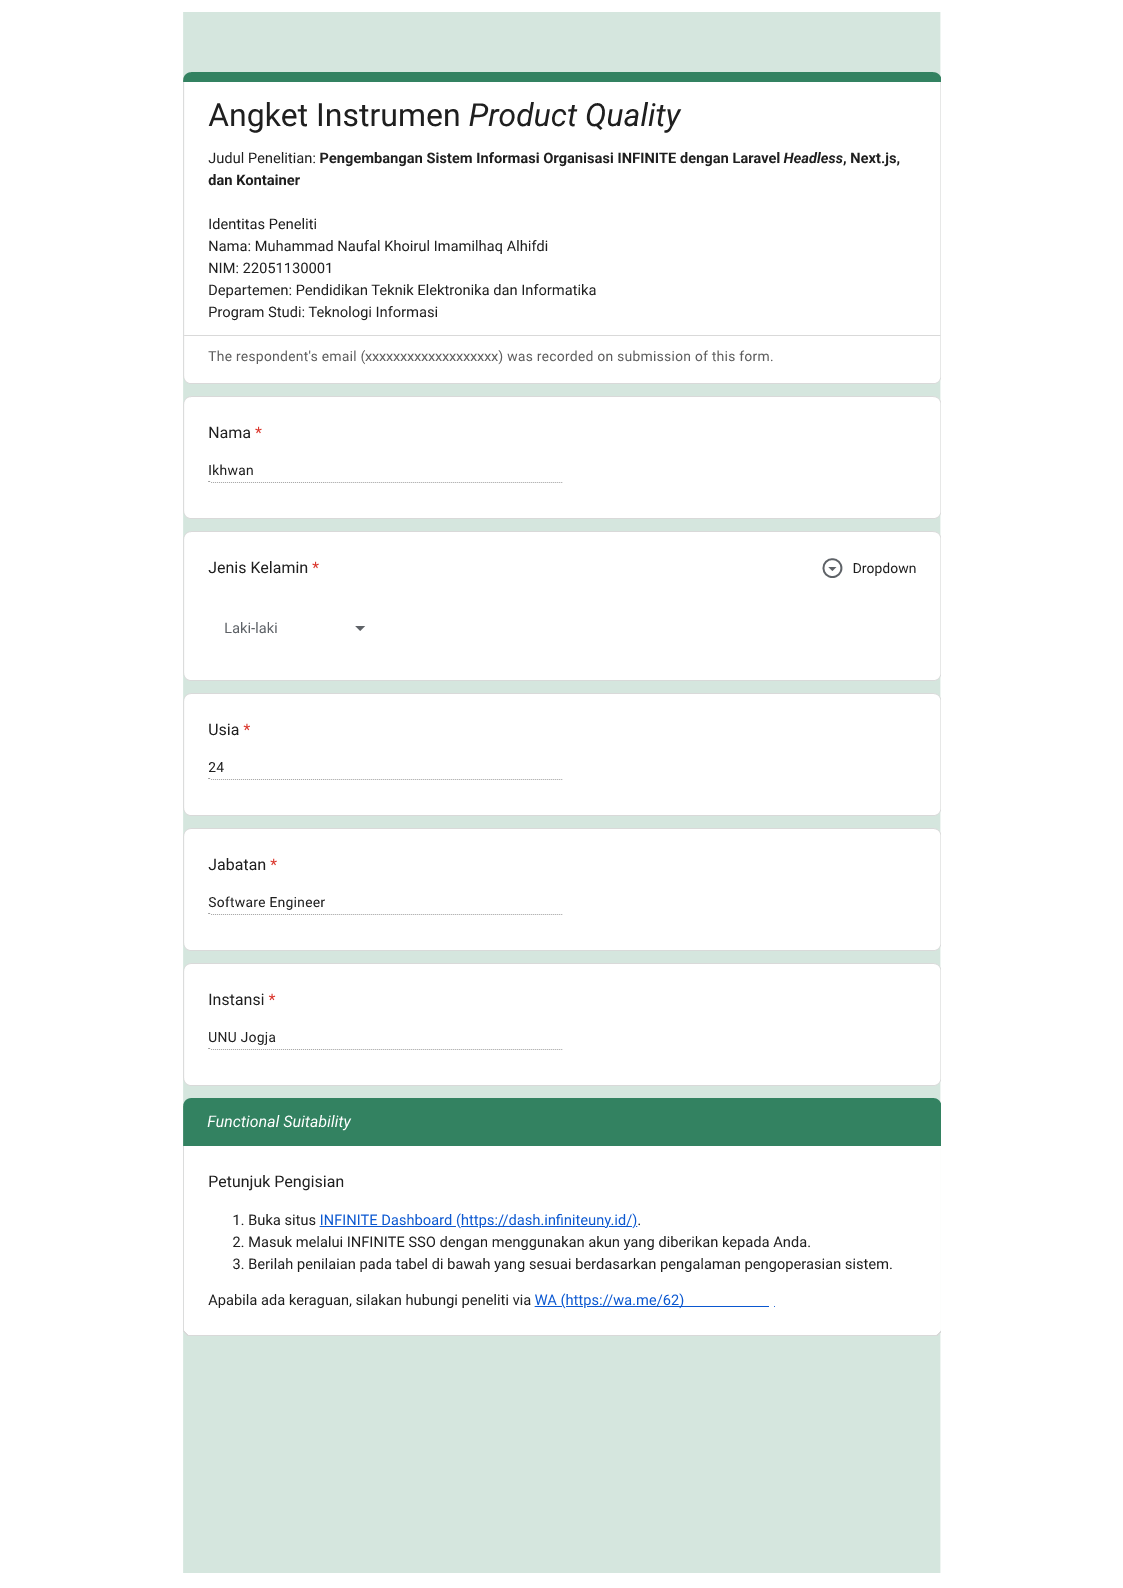
\includegraphics[width=1\textwidth,keepaspectratio]{images/product-quality-tests/hasil-product-quality-penguji-1-1.png}
\end{figure}

\begin{figure}[H]
      \centering
      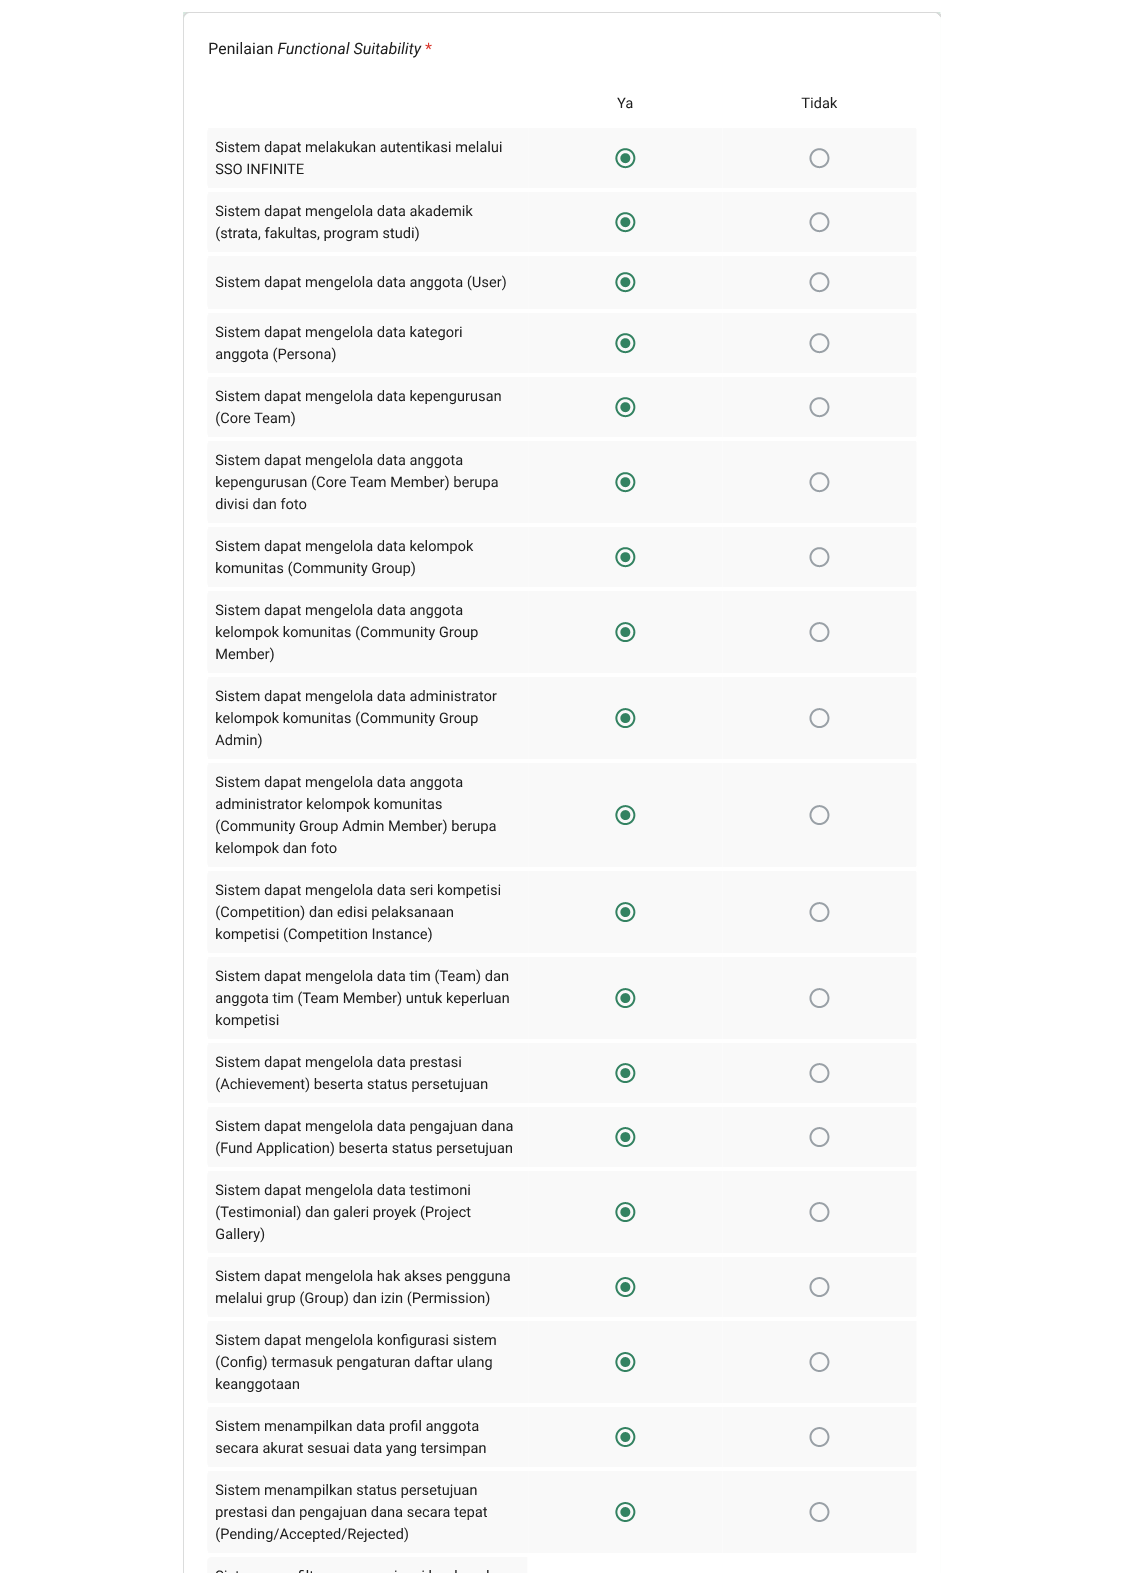
\includegraphics[width=1\textwidth,keepaspectratio]{images/product-quality-tests/hasil-product-quality-penguji-1-2.png}
\end{figure}

\begin{figure}[H]
      \centering
      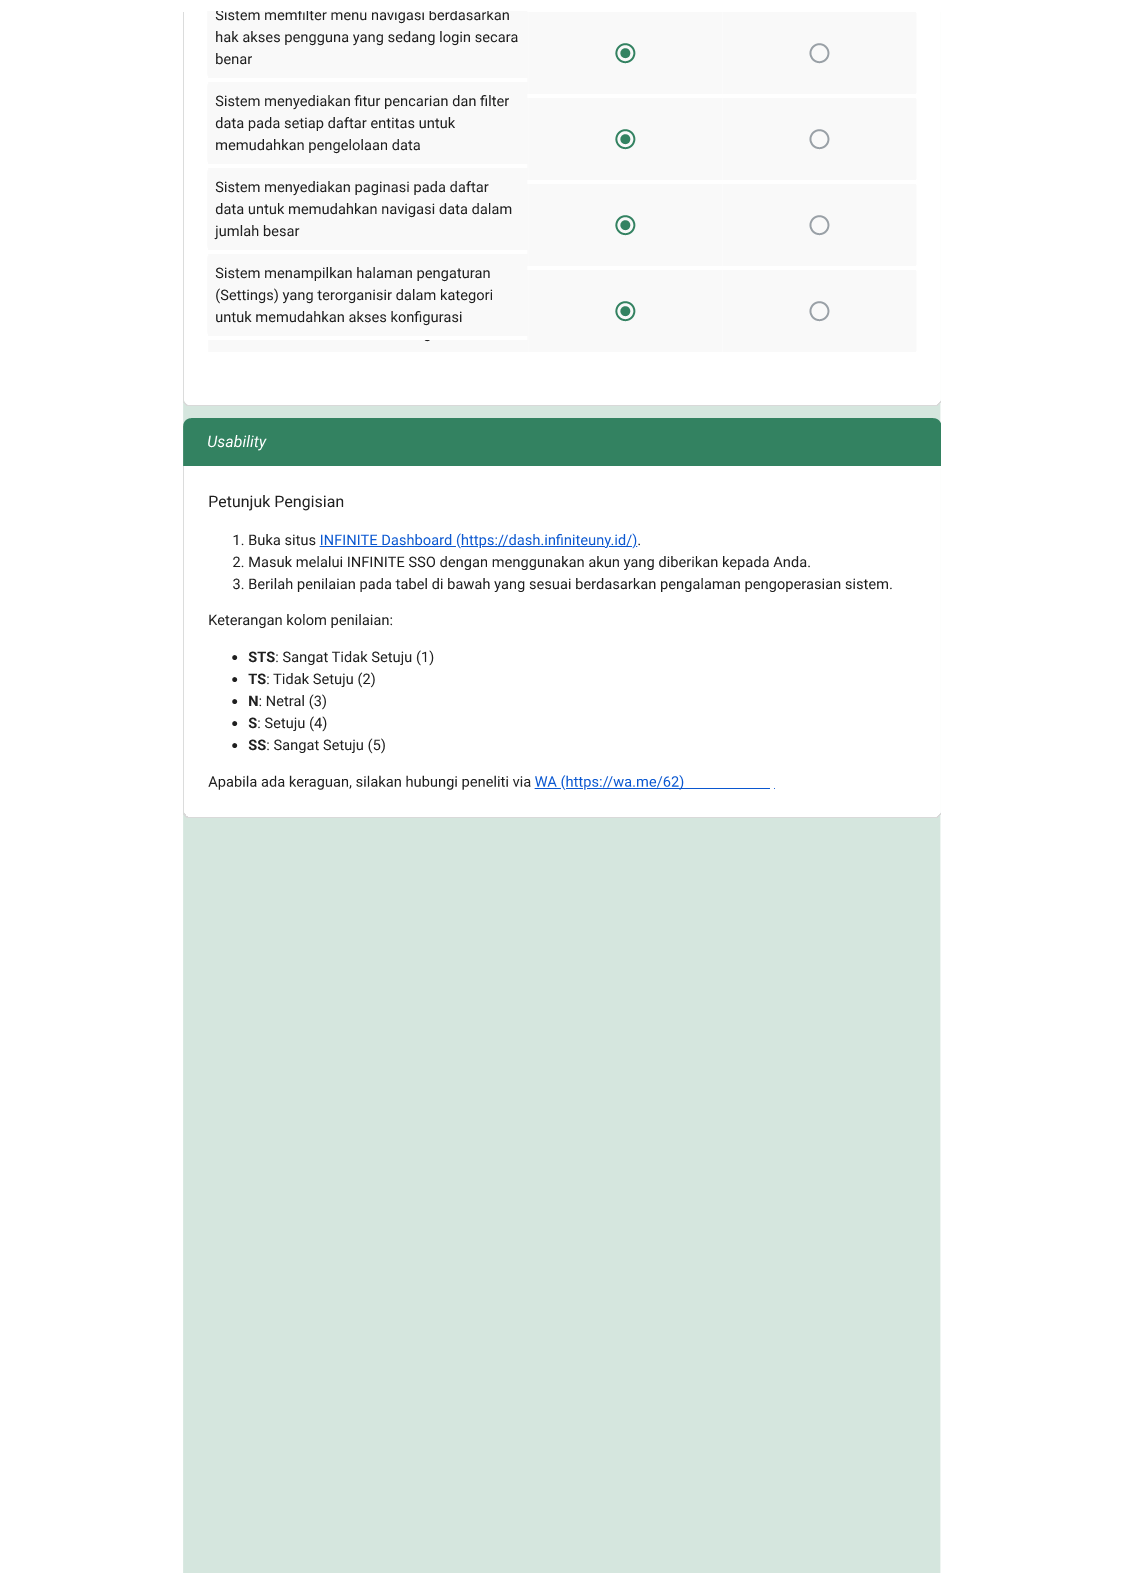
\includegraphics[width=1\textwidth,keepaspectratio]{images/product-quality-tests/hasil-product-quality-penguji-1-3.png}
\end{figure}

\begin{figure}[H]
      \centering
      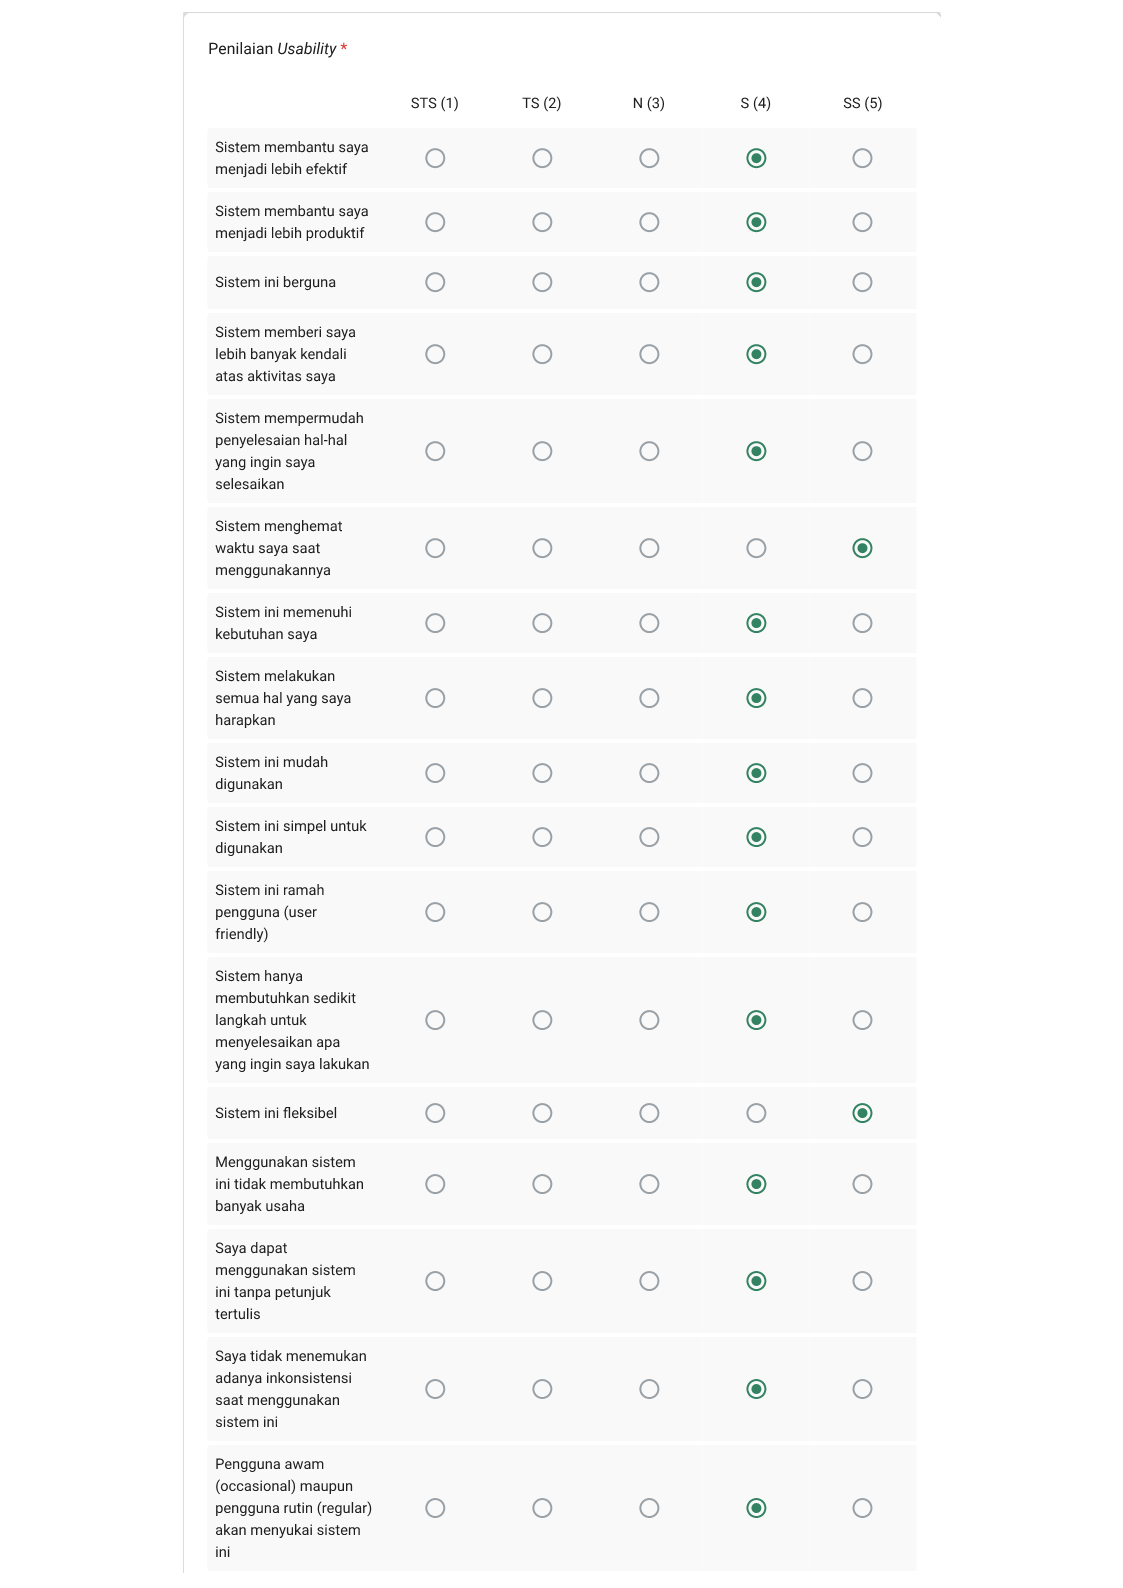
\includegraphics[width=1\textwidth,keepaspectratio]{images/product-quality-tests/hasil-product-quality-penguji-1-4.png}
\end{figure}

\begin{figure}[H]
      \centering
      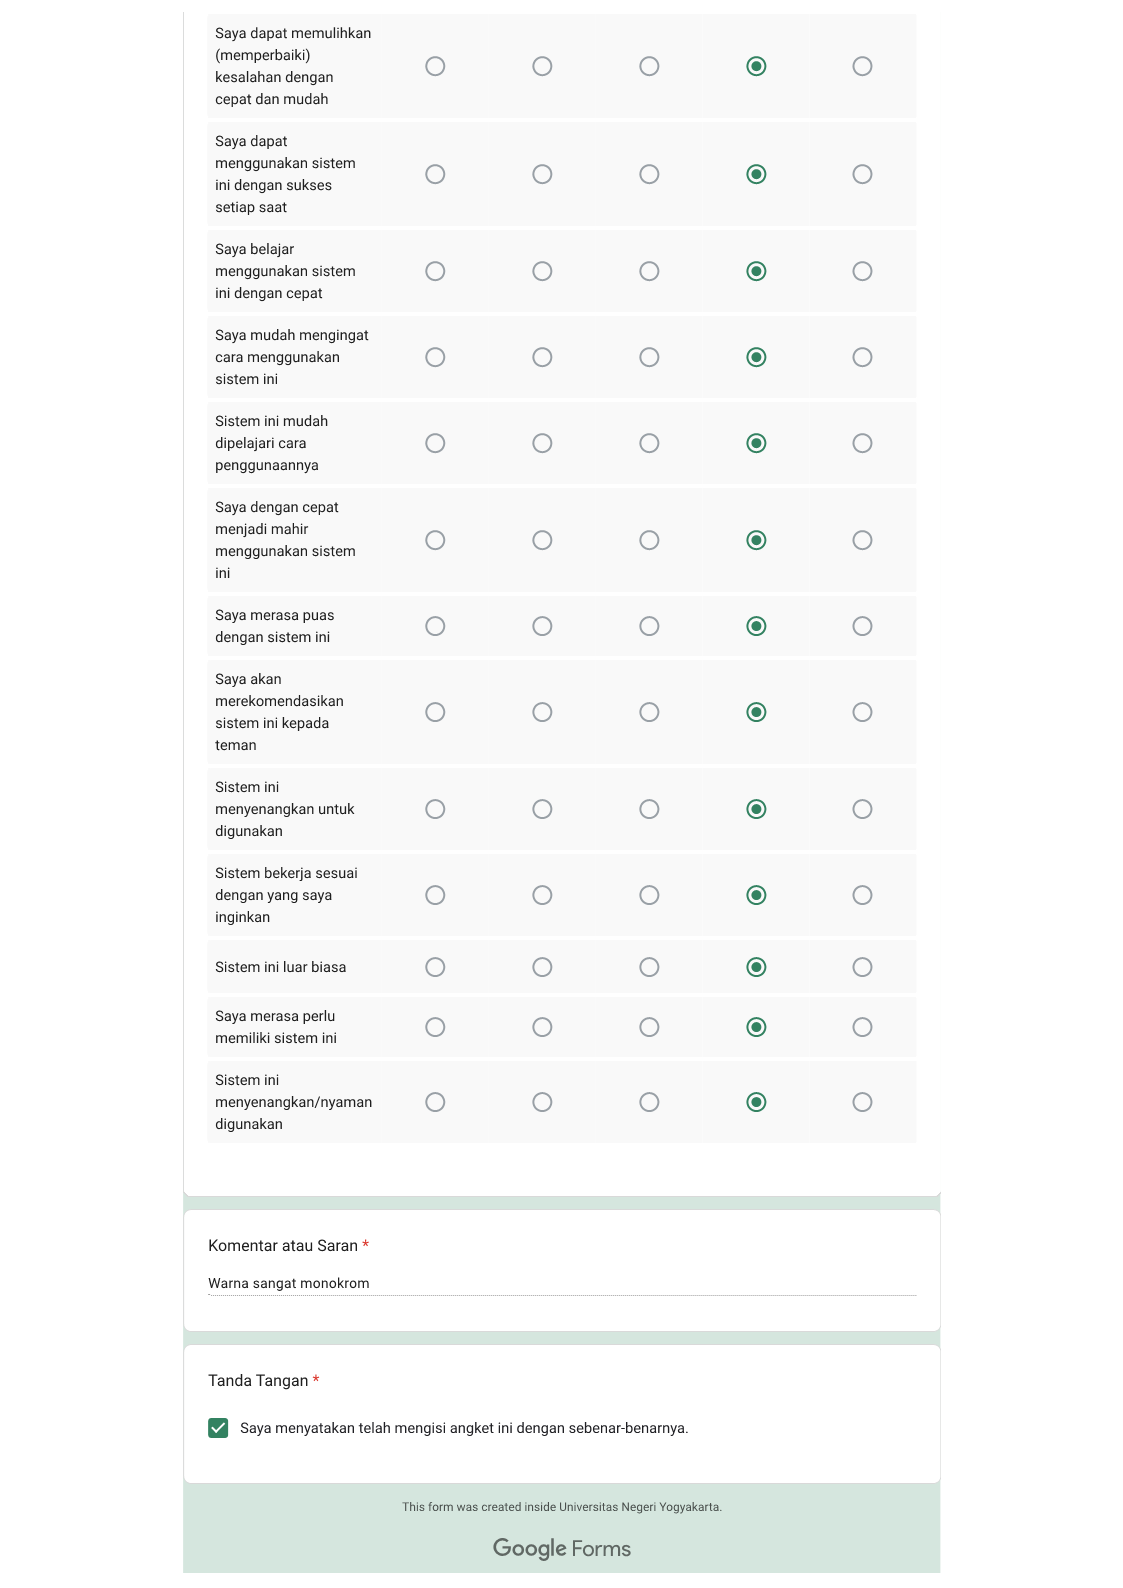
\includegraphics[width=1\textwidth,keepaspectratio]{images/product-quality-tests/hasil-product-quality-penguji-1-5.png}
\end{figure}

\newpage

\noindent Penguji 2

\begin{figure}[H]
      \centering
      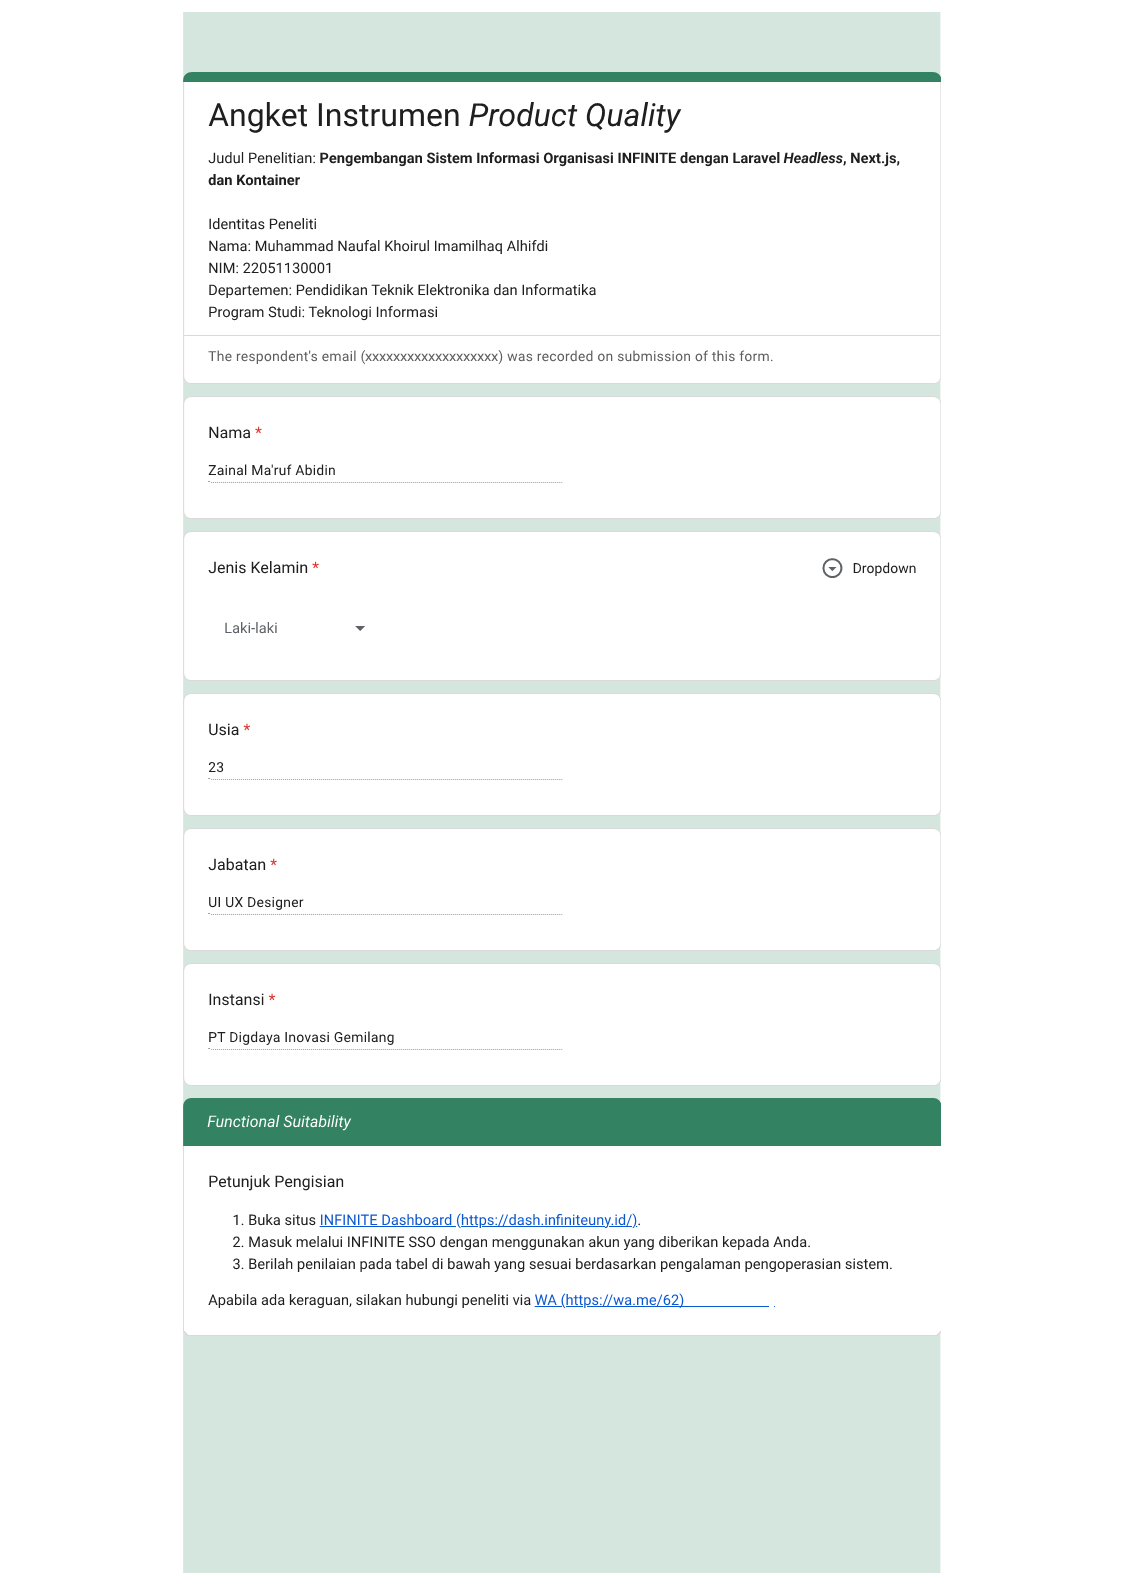
\includegraphics[width=1\textwidth,keepaspectratio]{images/product-quality-tests/hasil-product-quality-penguji-2-1.png}
\end{figure}

\begin{figure}[H]
      \centering
      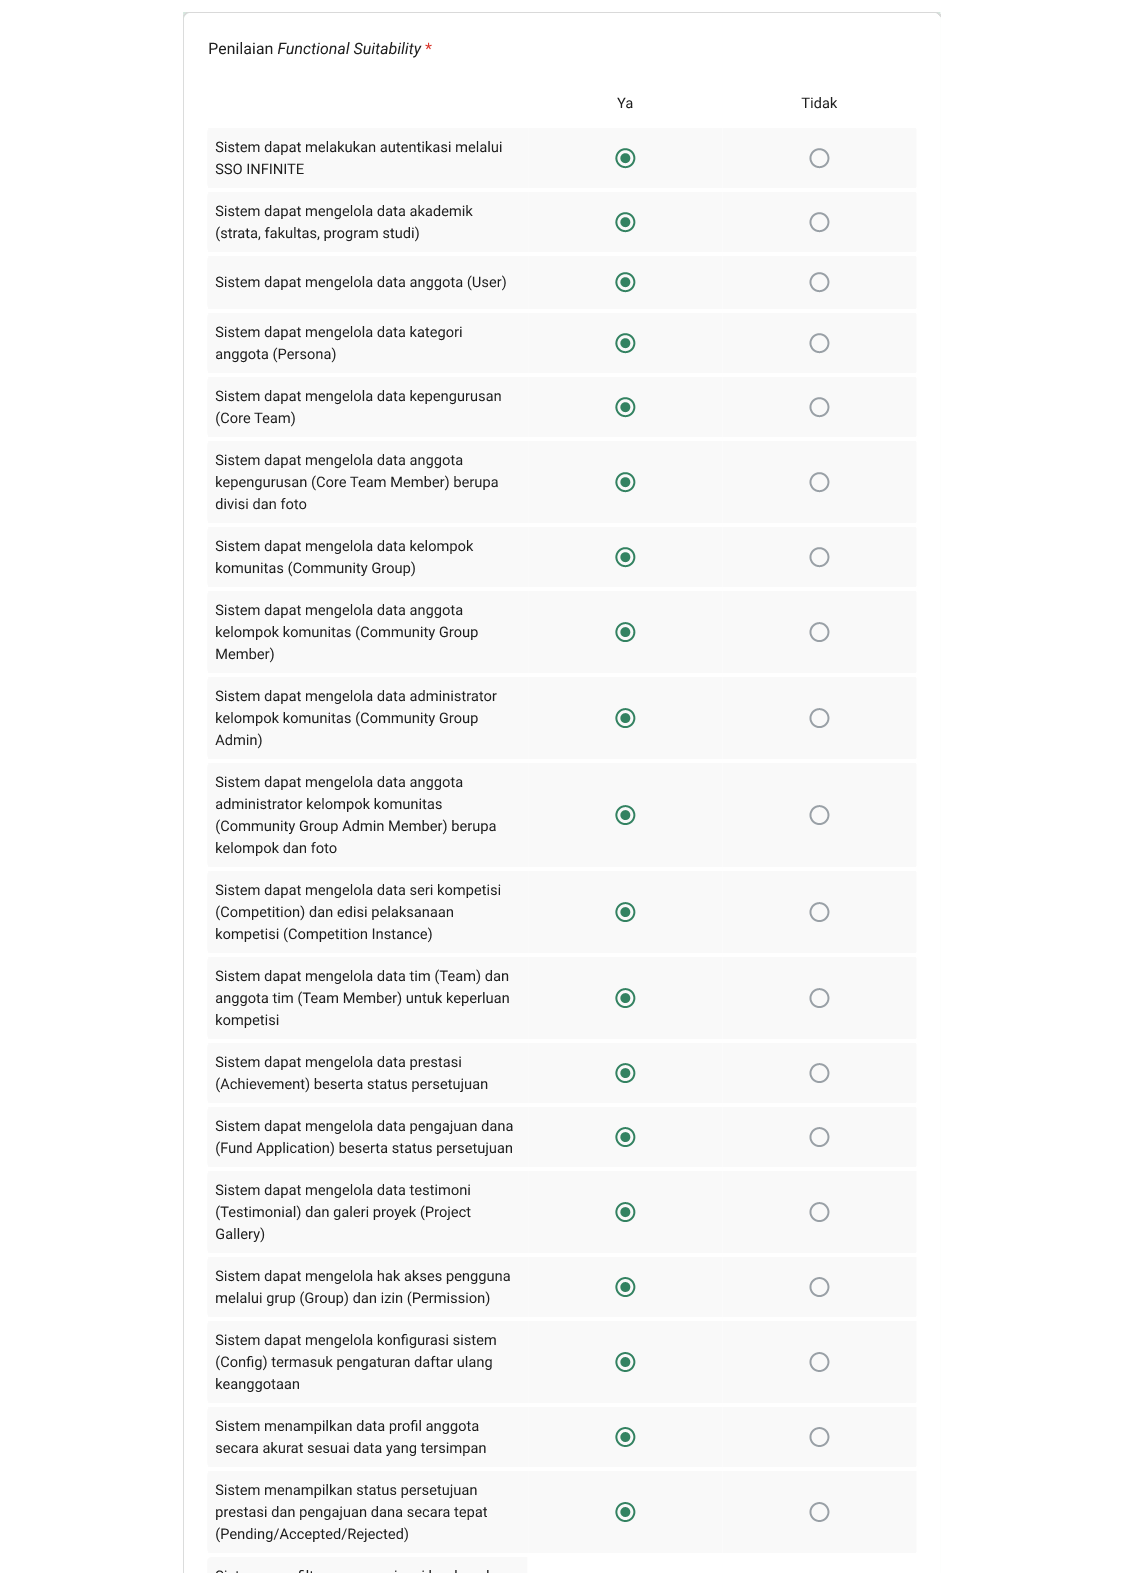
\includegraphics[width=1\textwidth,keepaspectratio]{images/product-quality-tests/hasil-product-quality-penguji-2-2.png}
\end{figure}

\begin{figure}[H]
      \centering
      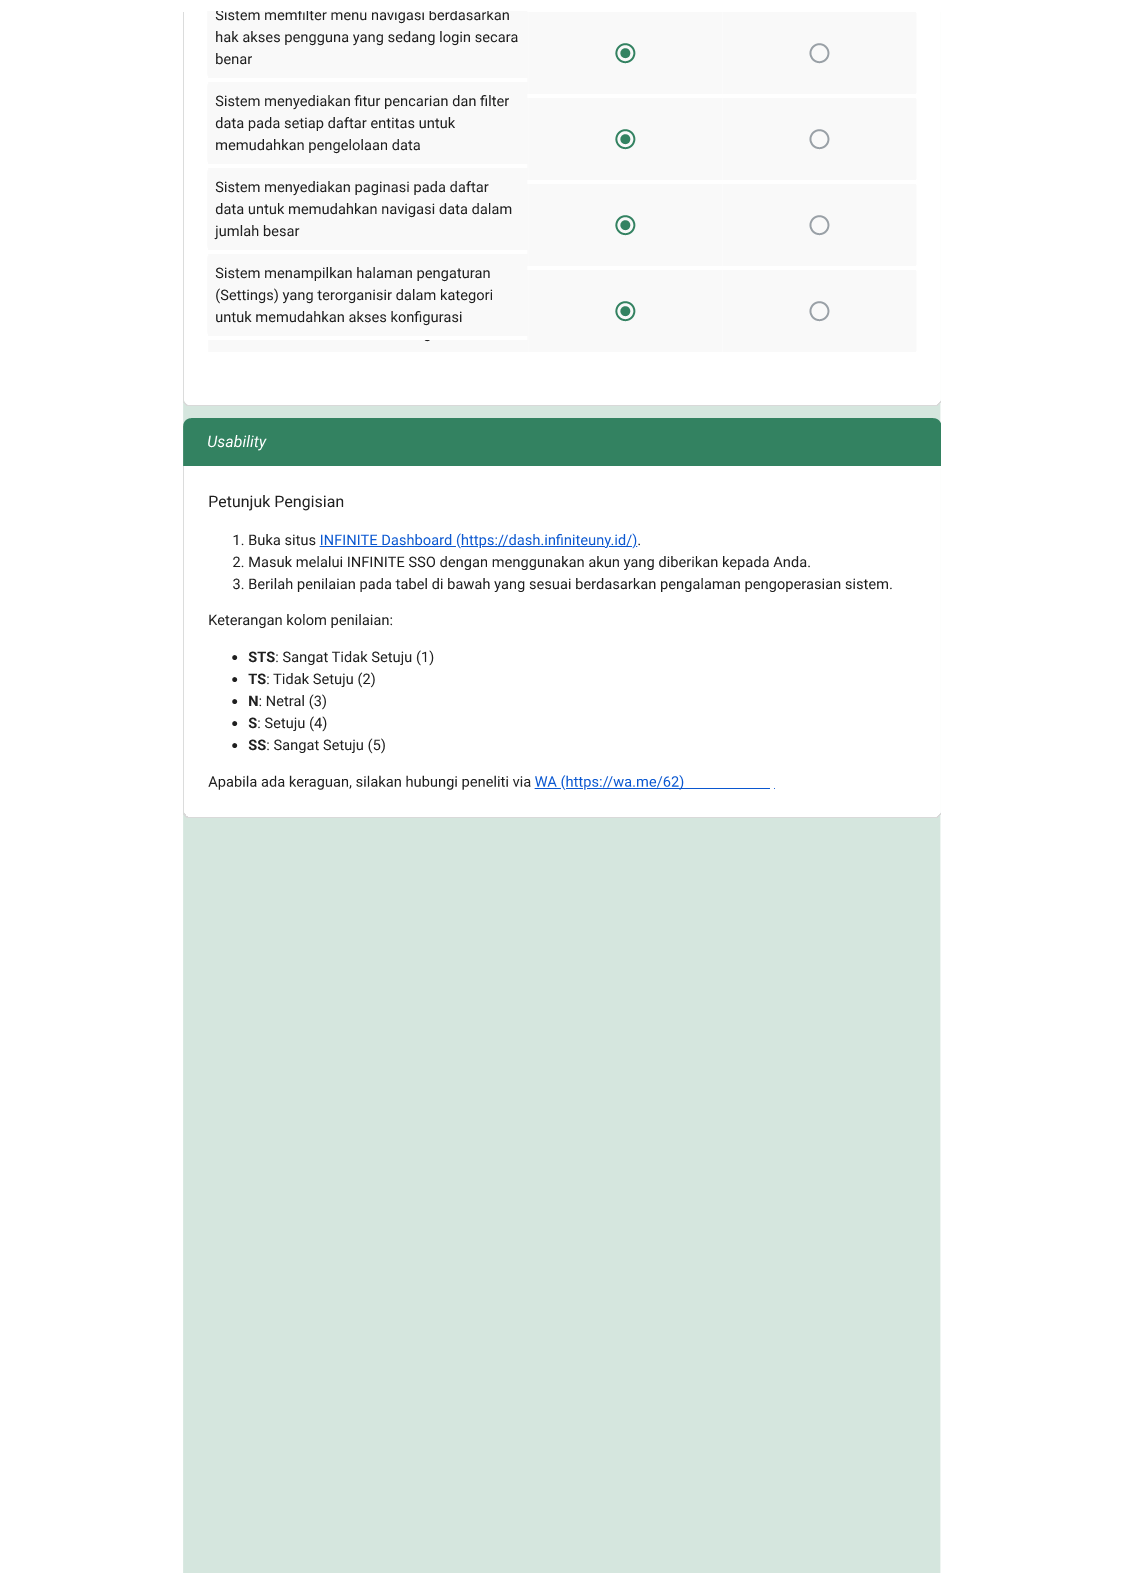
\includegraphics[width=1\textwidth,keepaspectratio]{images/product-quality-tests/hasil-product-quality-penguji-2-3.png}
\end{figure}

\begin{figure}[H]
      \centering
      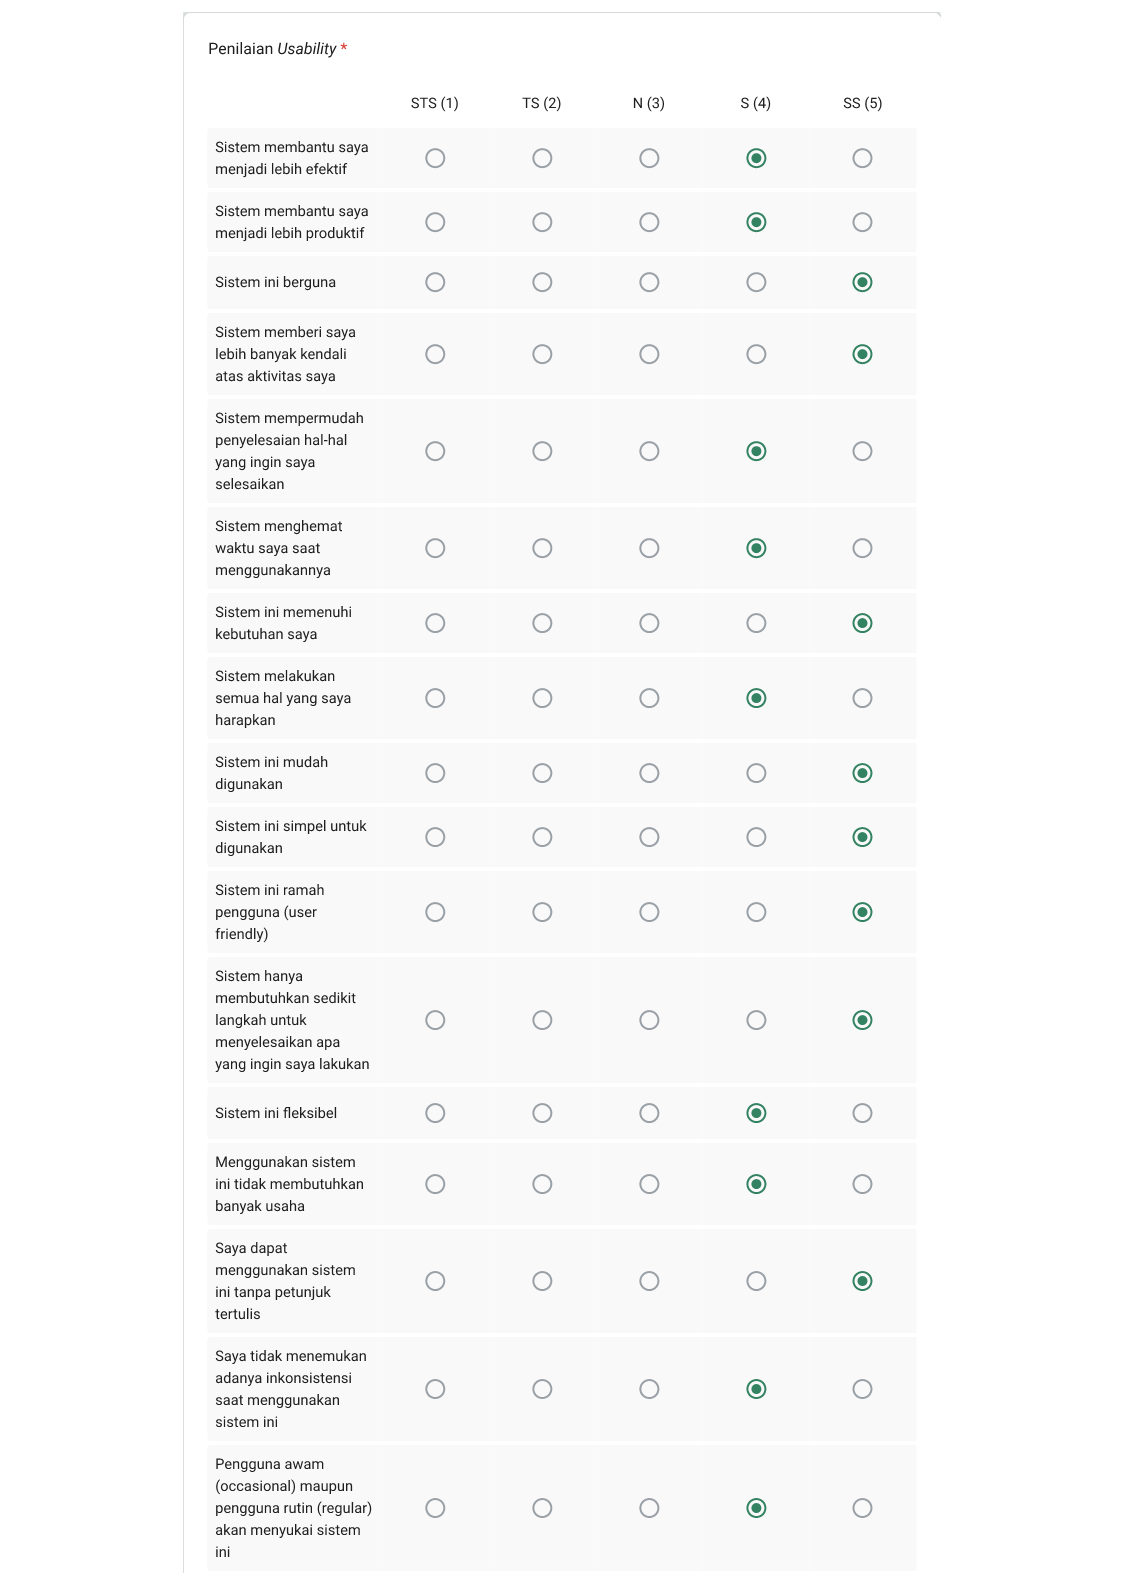
\includegraphics[width=1\textwidth,keepaspectratio]{images/product-quality-tests/hasil-product-quality-penguji-2-4.png}
\end{figure}

\begin{figure}[H]
      \centering
      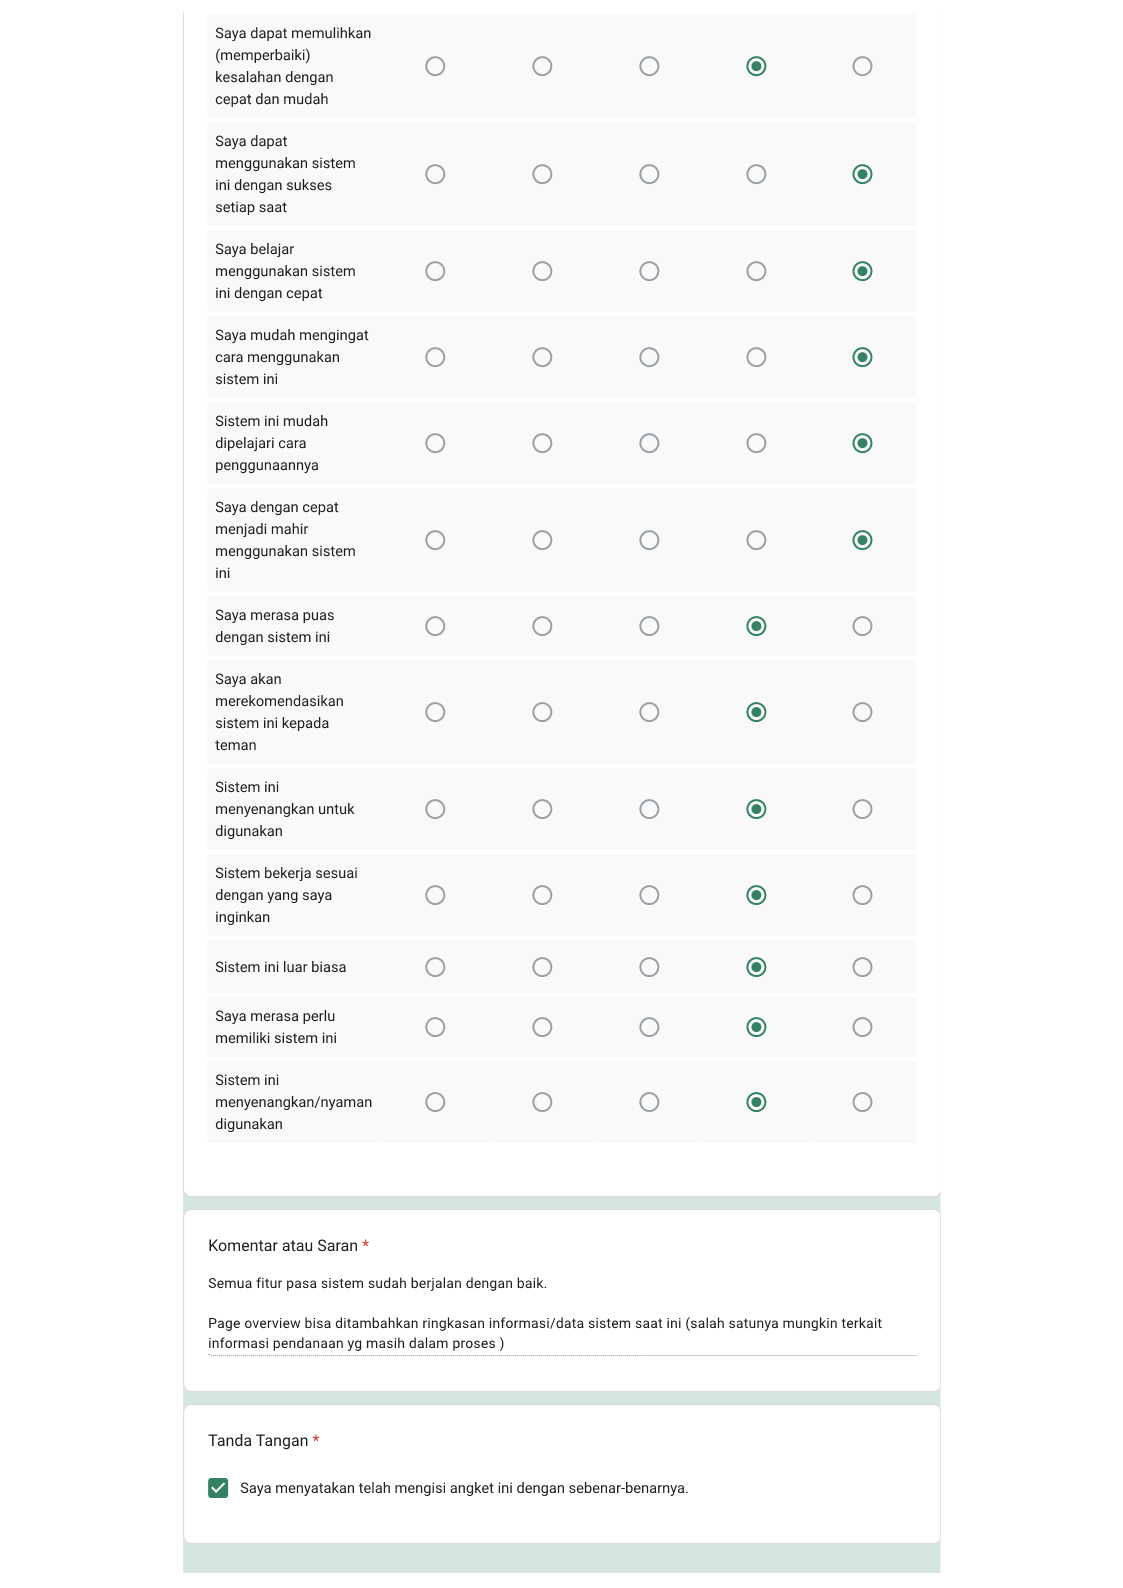
\includegraphics[width=1\textwidth,keepaspectratio]{images/product-quality-tests/hasil-product-quality-penguji-2-5.png}
\end{figure}

\newpage

\noindent Penguji 3

\begin{figure}[H]
      \centering
      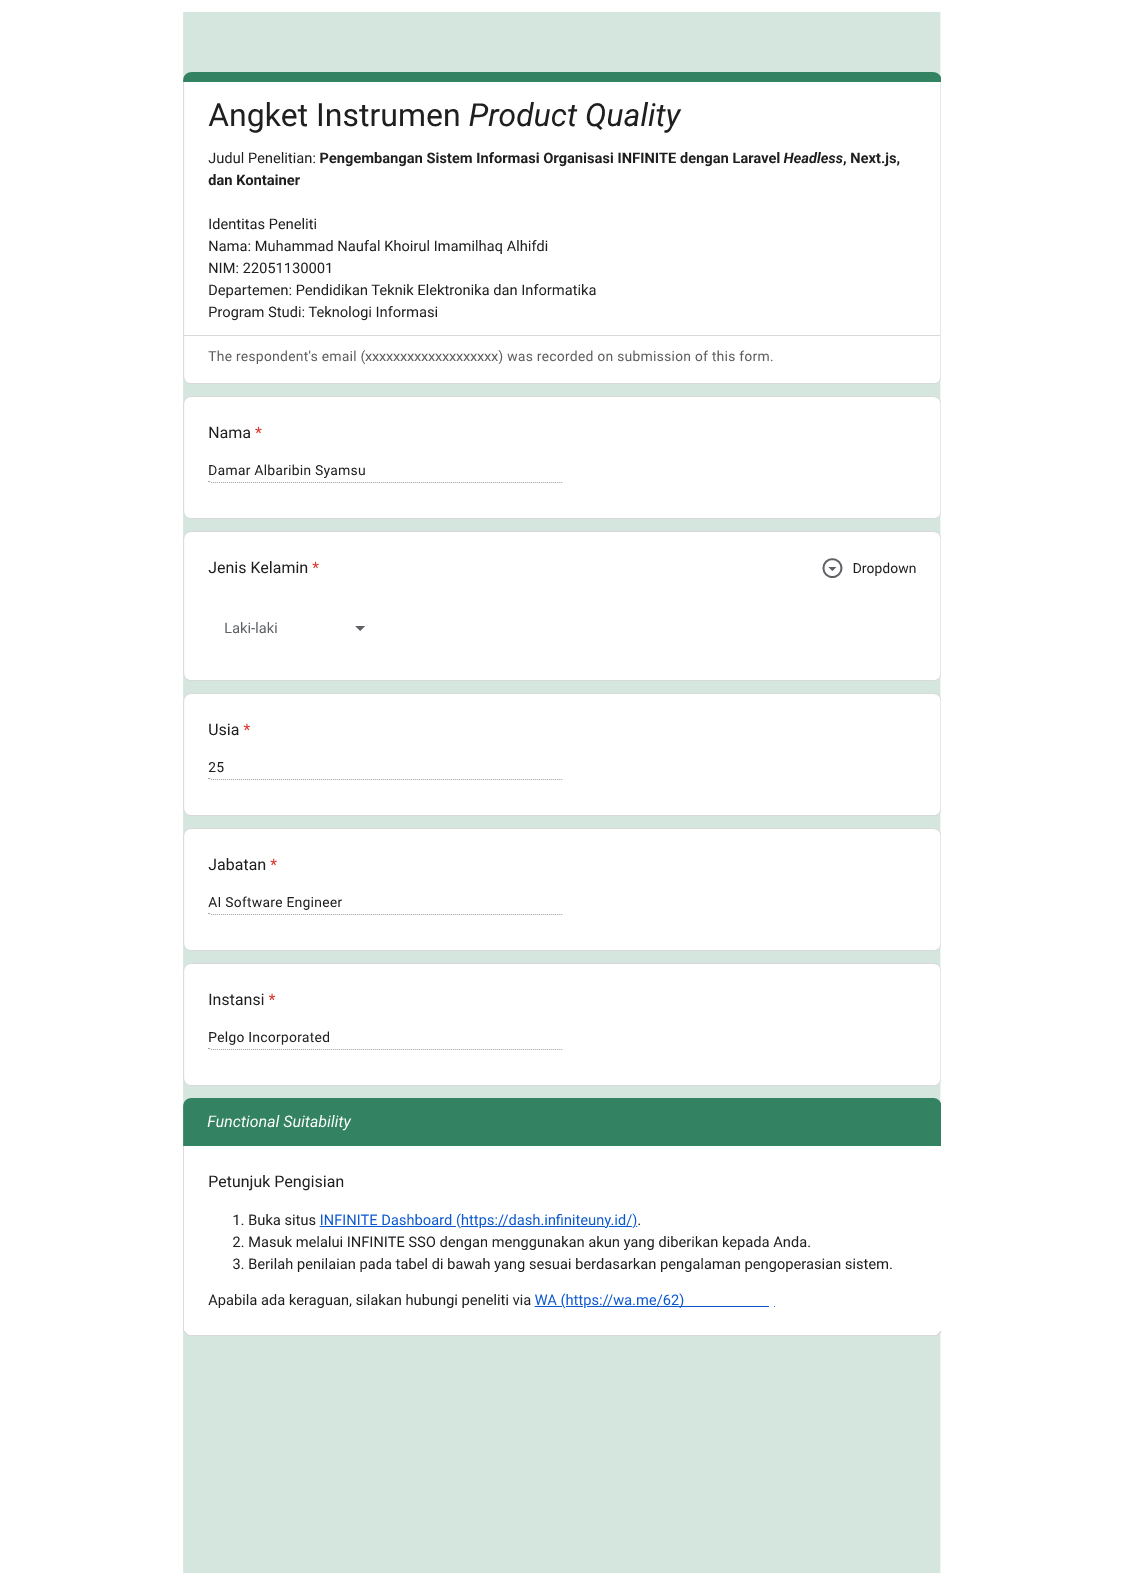
\includegraphics[width=1\textwidth,keepaspectratio]{images/product-quality-tests/hasil-product-quality-penguji-3-1.png}
\end{figure}

\begin{figure}[H]
      \centering
      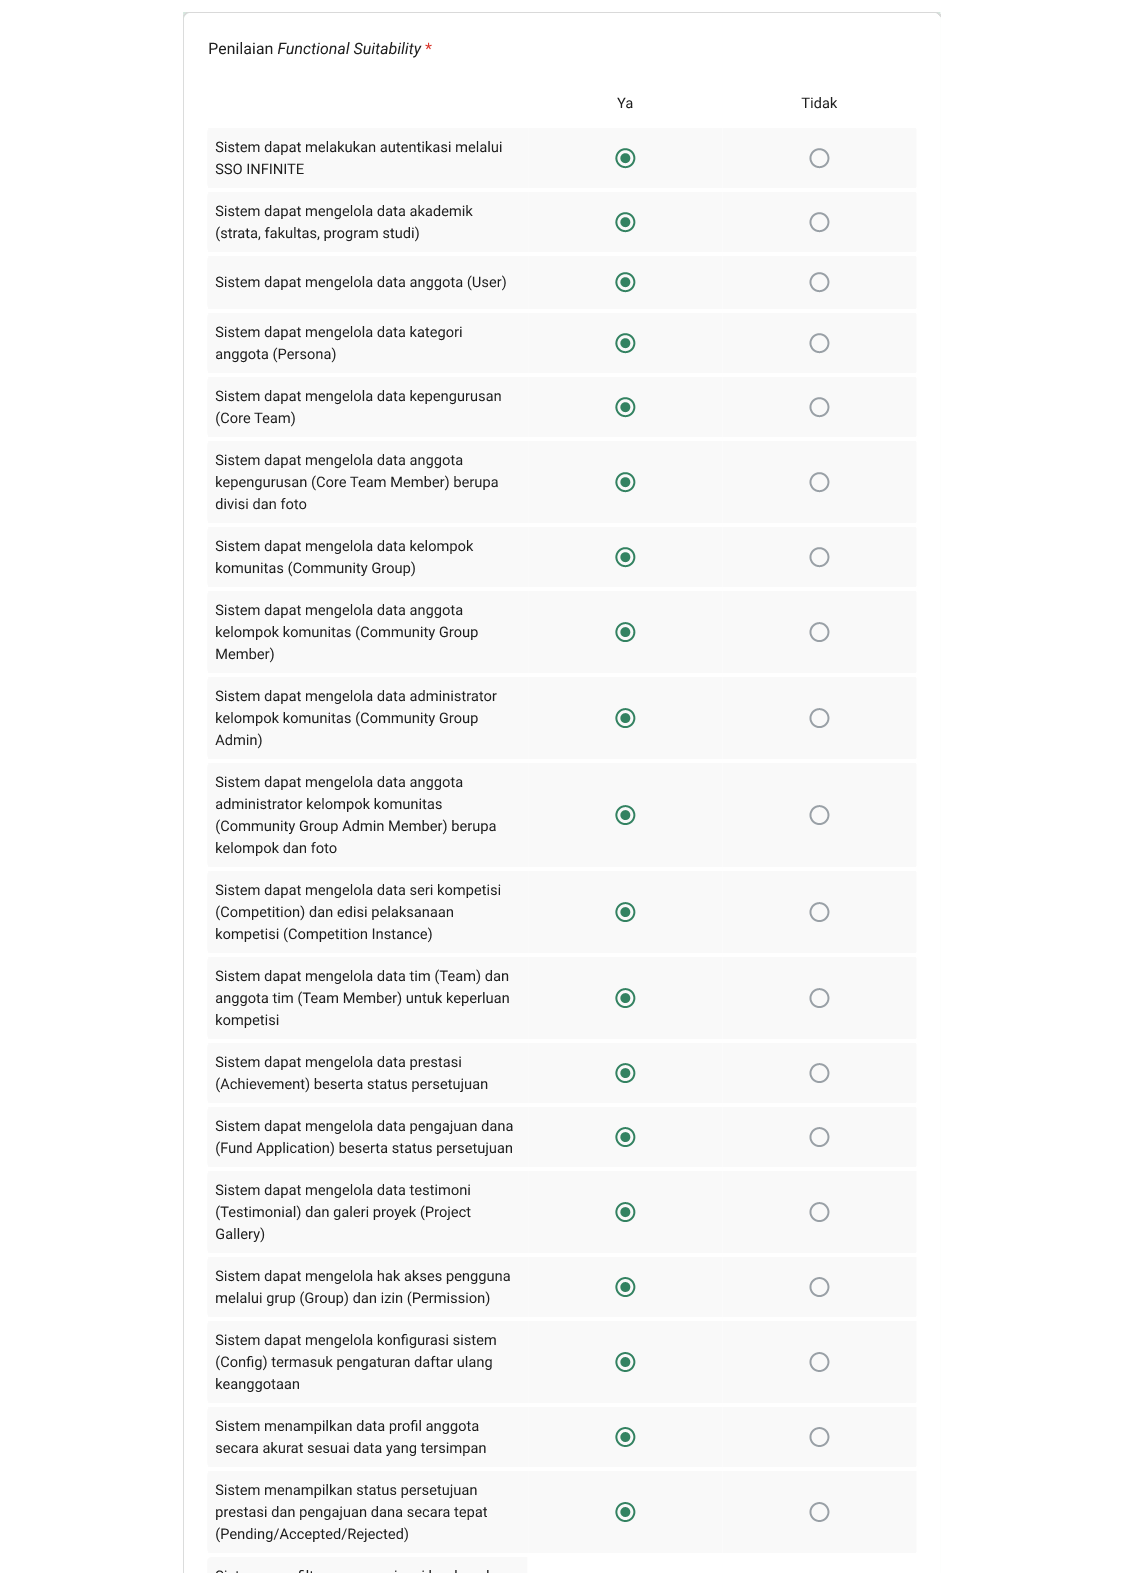
\includegraphics[width=1\textwidth,keepaspectratio]{images/product-quality-tests/hasil-product-quality-penguji-3-2.png}
\end{figure}

\begin{figure}[H]
      \centering
      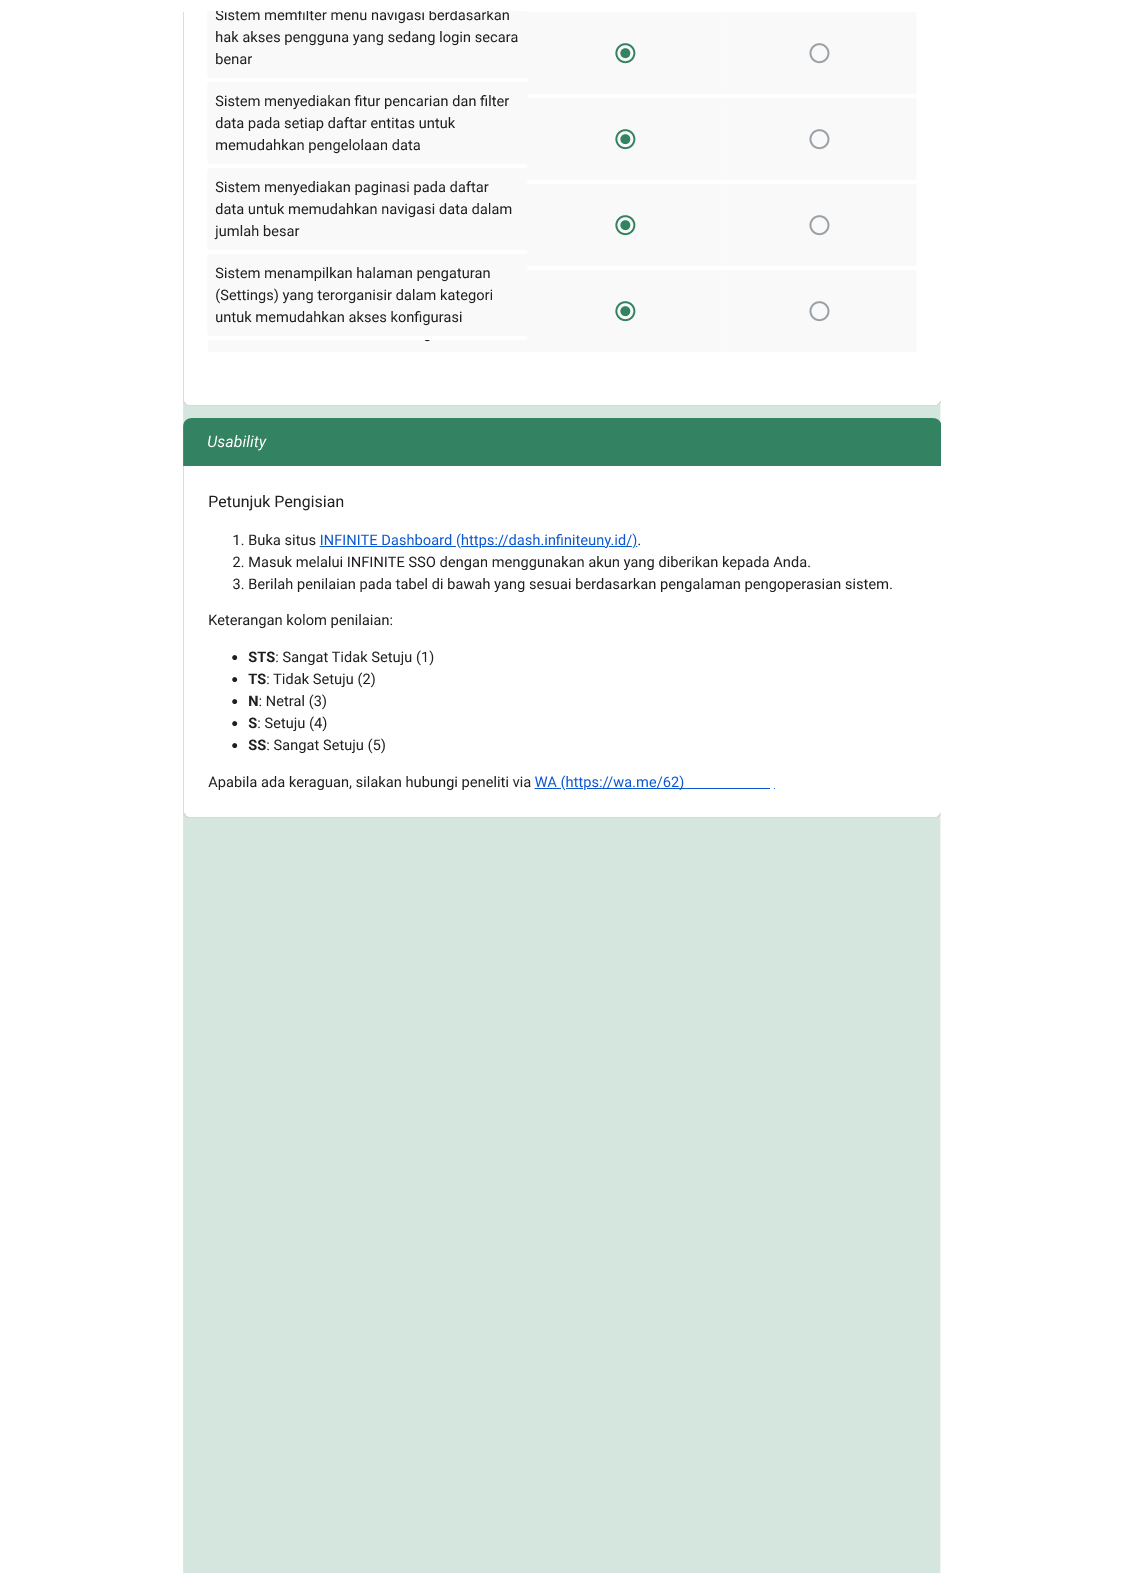
\includegraphics[width=1\textwidth,keepaspectratio]{images/product-quality-tests/hasil-product-quality-penguji-3-3.png}
\end{figure}

\begin{figure}[H]
      \centering
      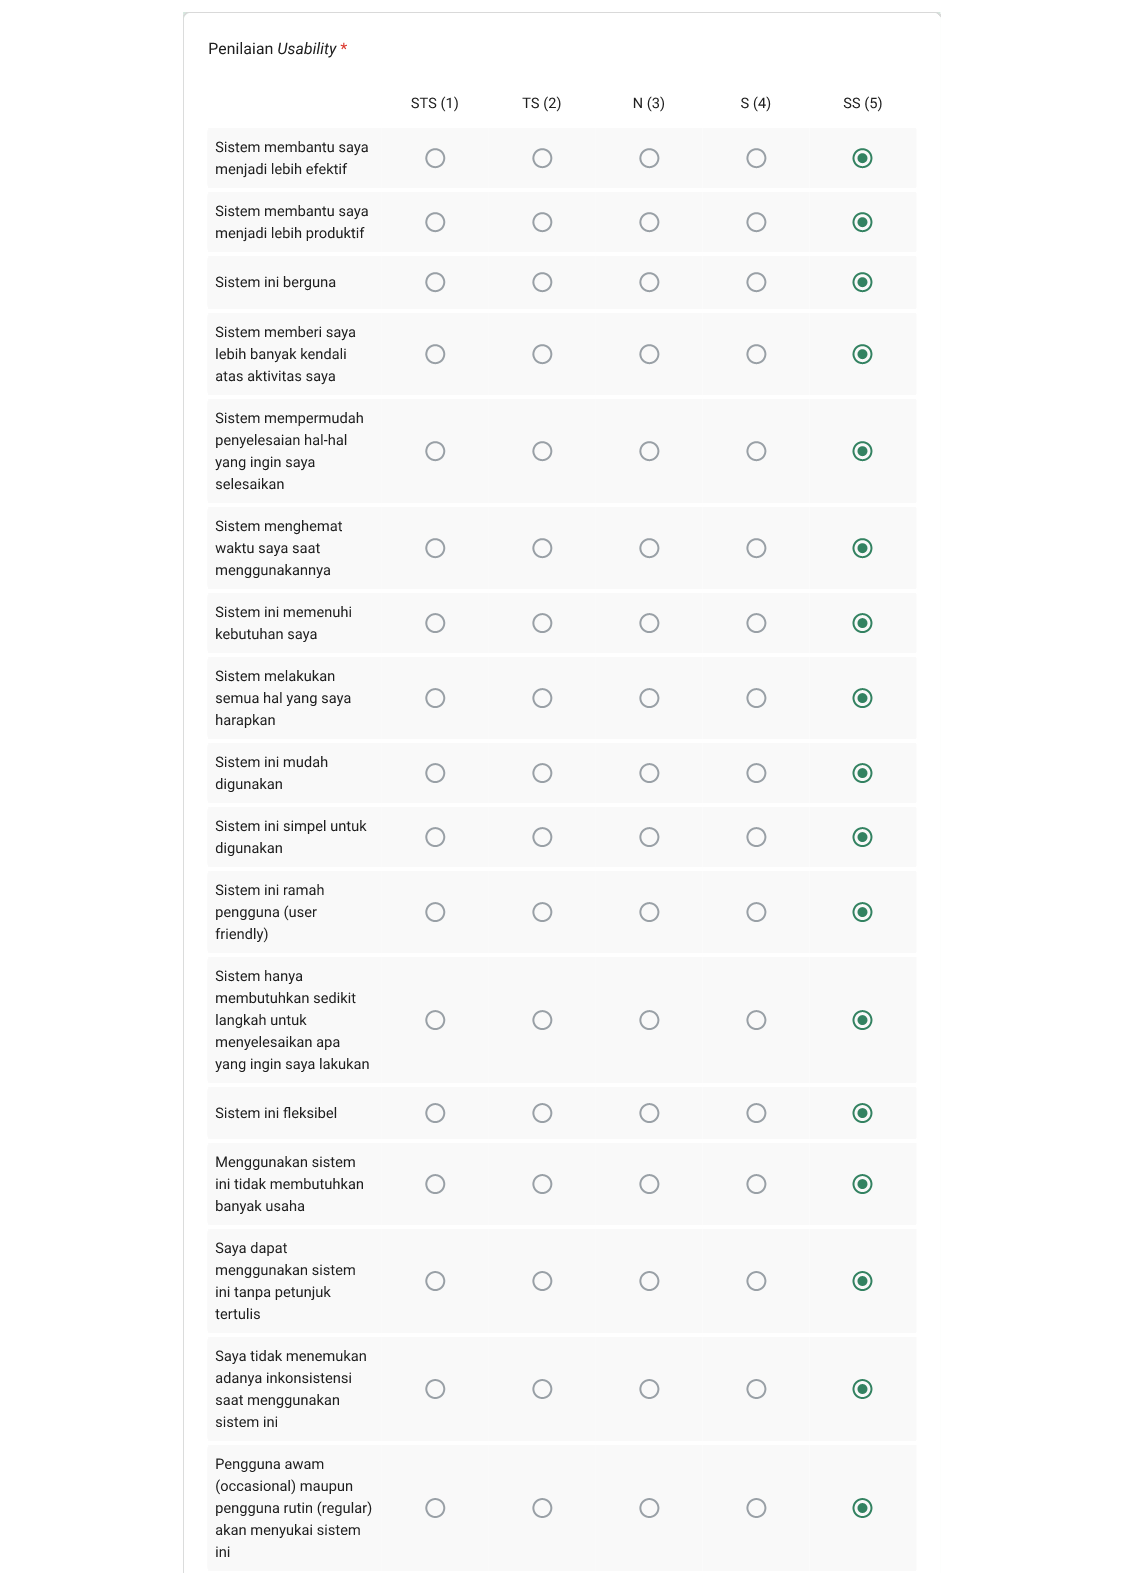
\includegraphics[width=1\textwidth,keepaspectratio]{images/product-quality-tests/hasil-product-quality-penguji-3-4.png}
\end{figure}

\begin{figure}[H]
      \centering
      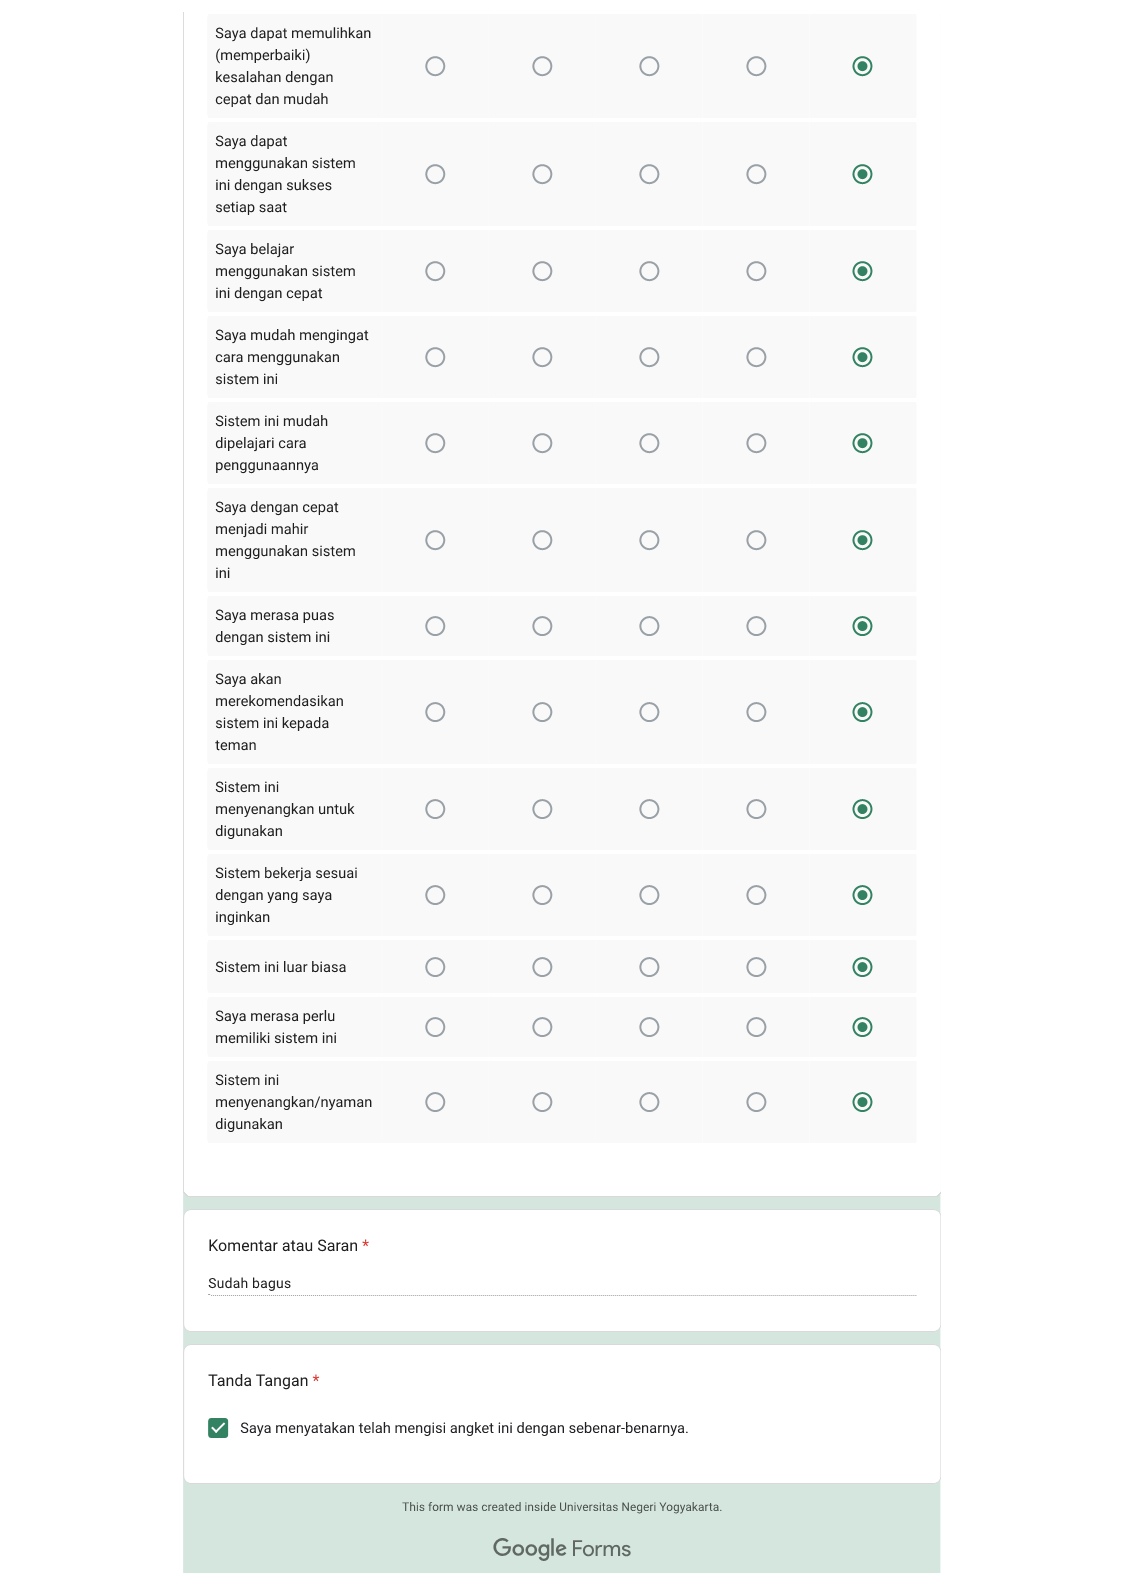
\includegraphics[width=1\textwidth,keepaspectratio]{images/product-quality-tests/hasil-product-quality-penguji-3-5.png}
\end{figure}

\newpage

\noindent Penguji 4

\begin{figure}[H]
      \centering
      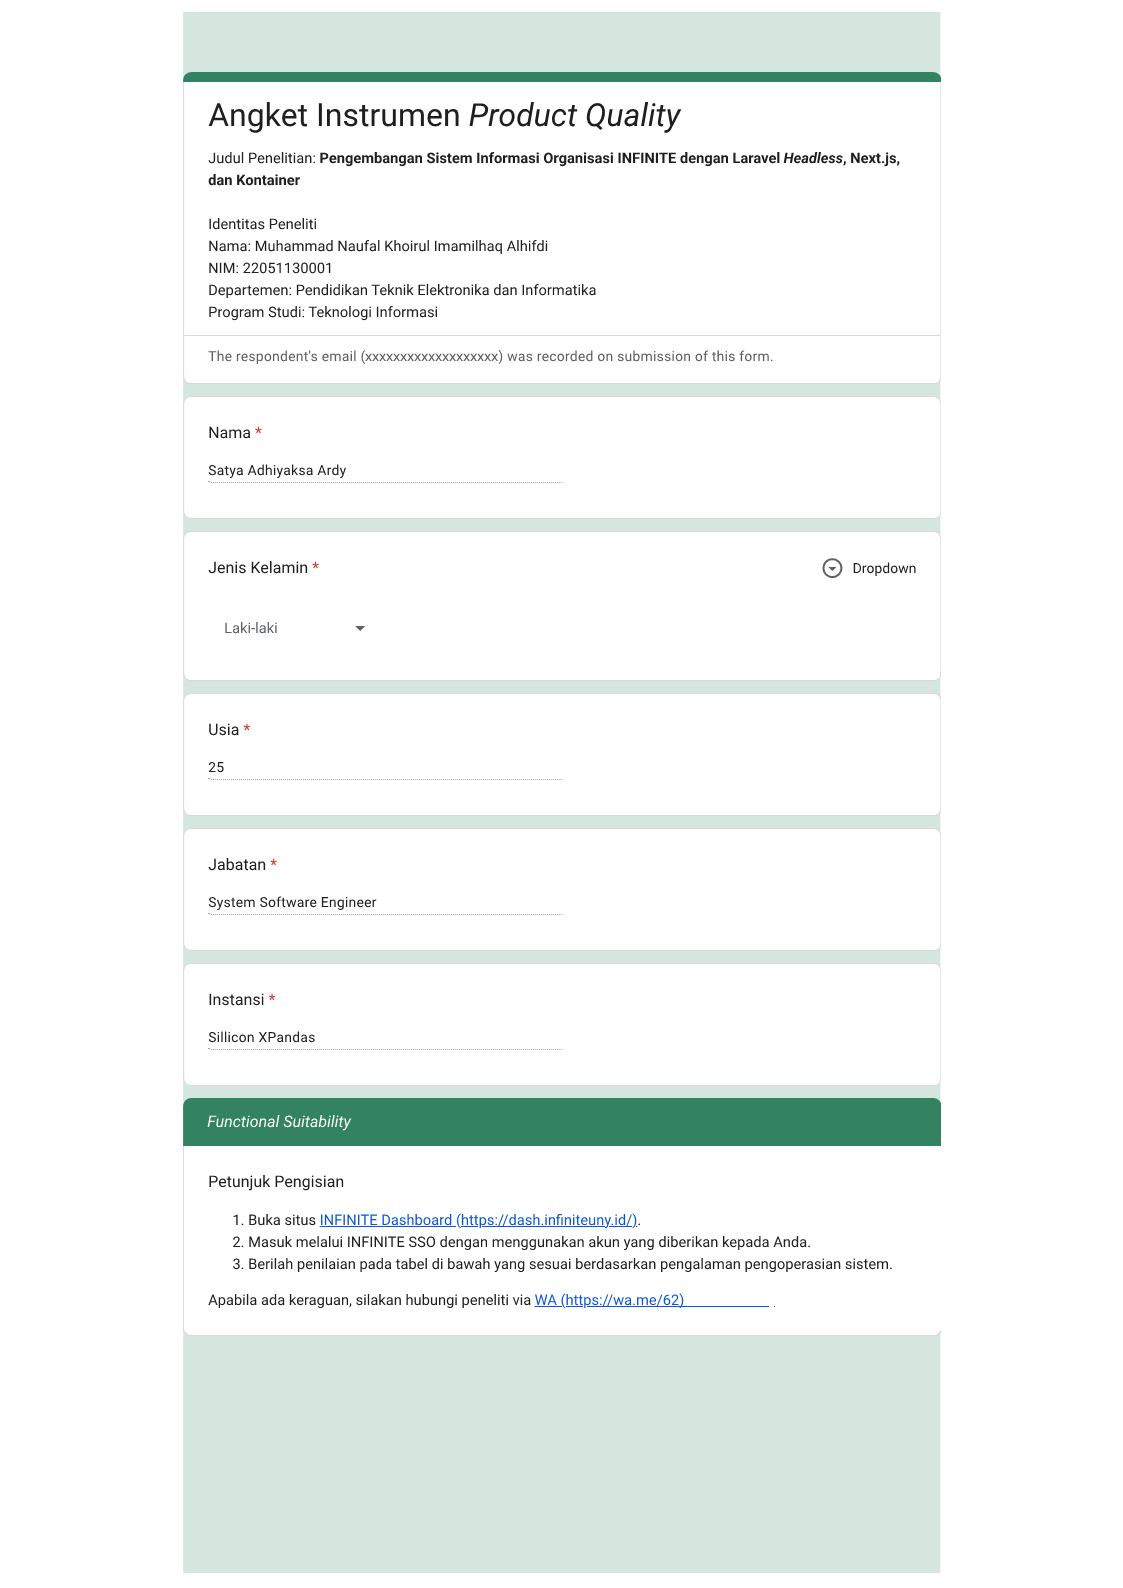
\includegraphics[width=1\textwidth,keepaspectratio]{images/product-quality-tests/hasil-product-quality-penguji-4-1.png}
\end{figure}

\begin{figure}[H]
      \centering
      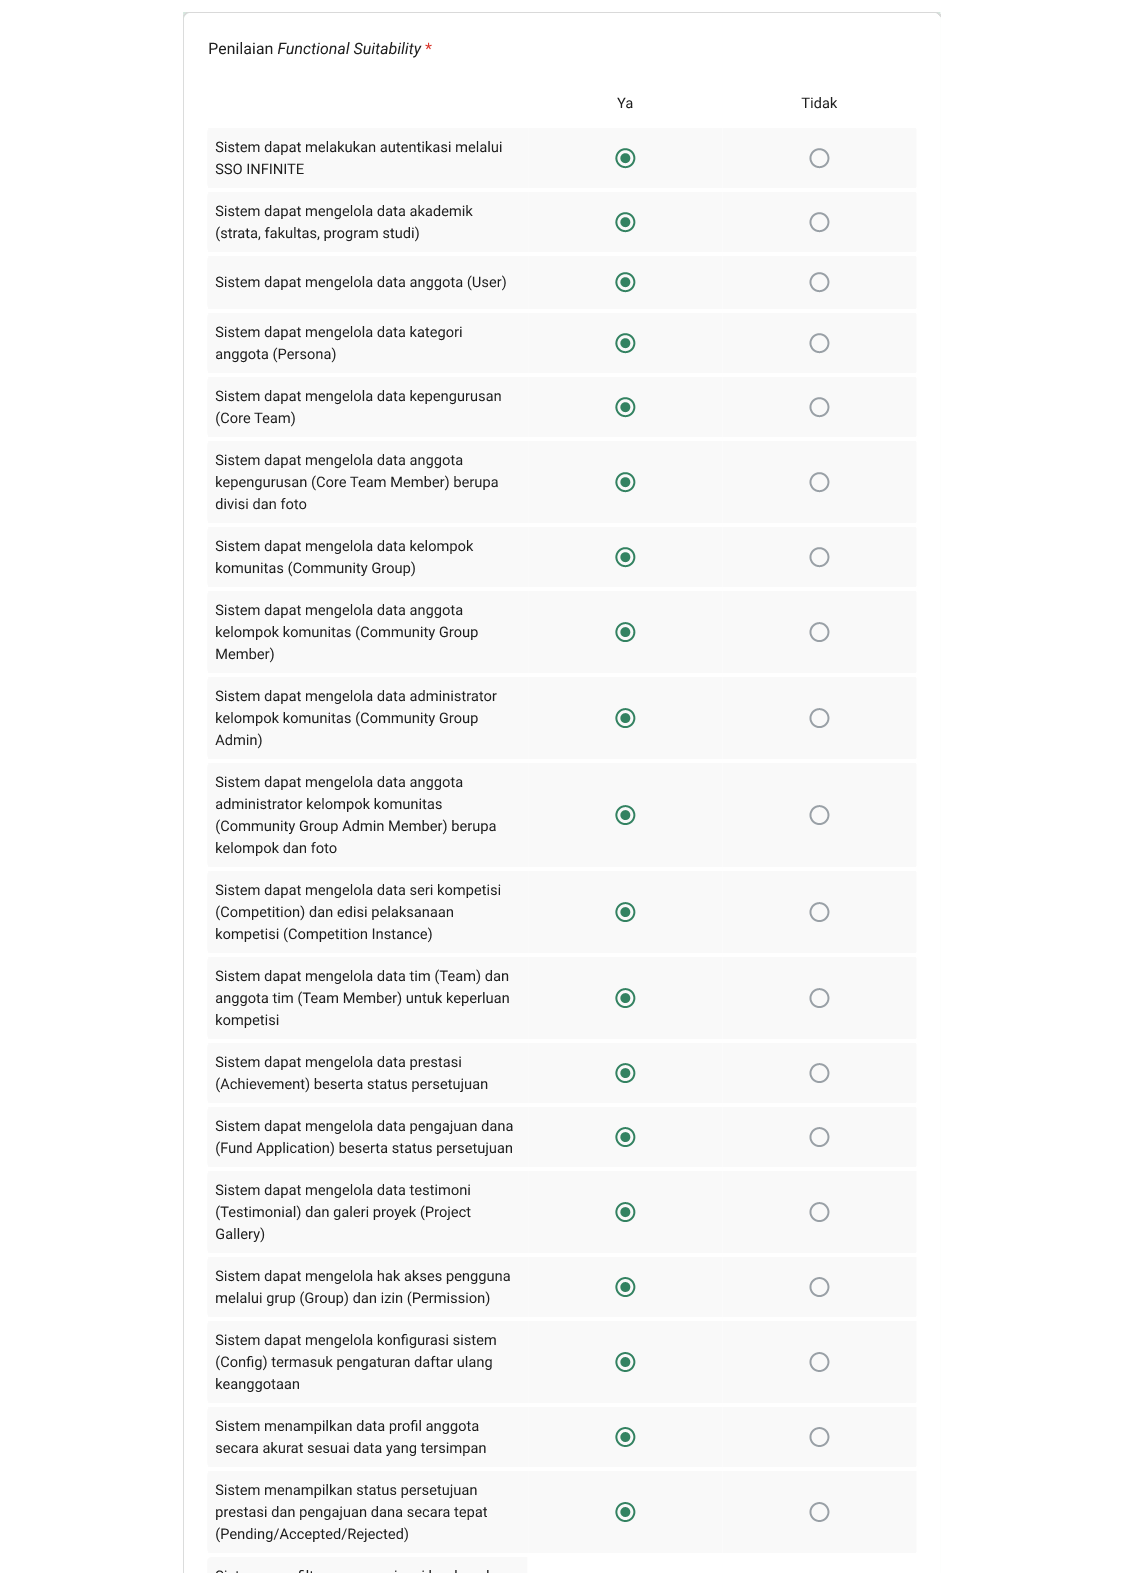
\includegraphics[width=1\textwidth,keepaspectratio]{images/product-quality-tests/hasil-product-quality-penguji-4-2.png}
\end{figure}

\begin{figure}[H]
      \centering
      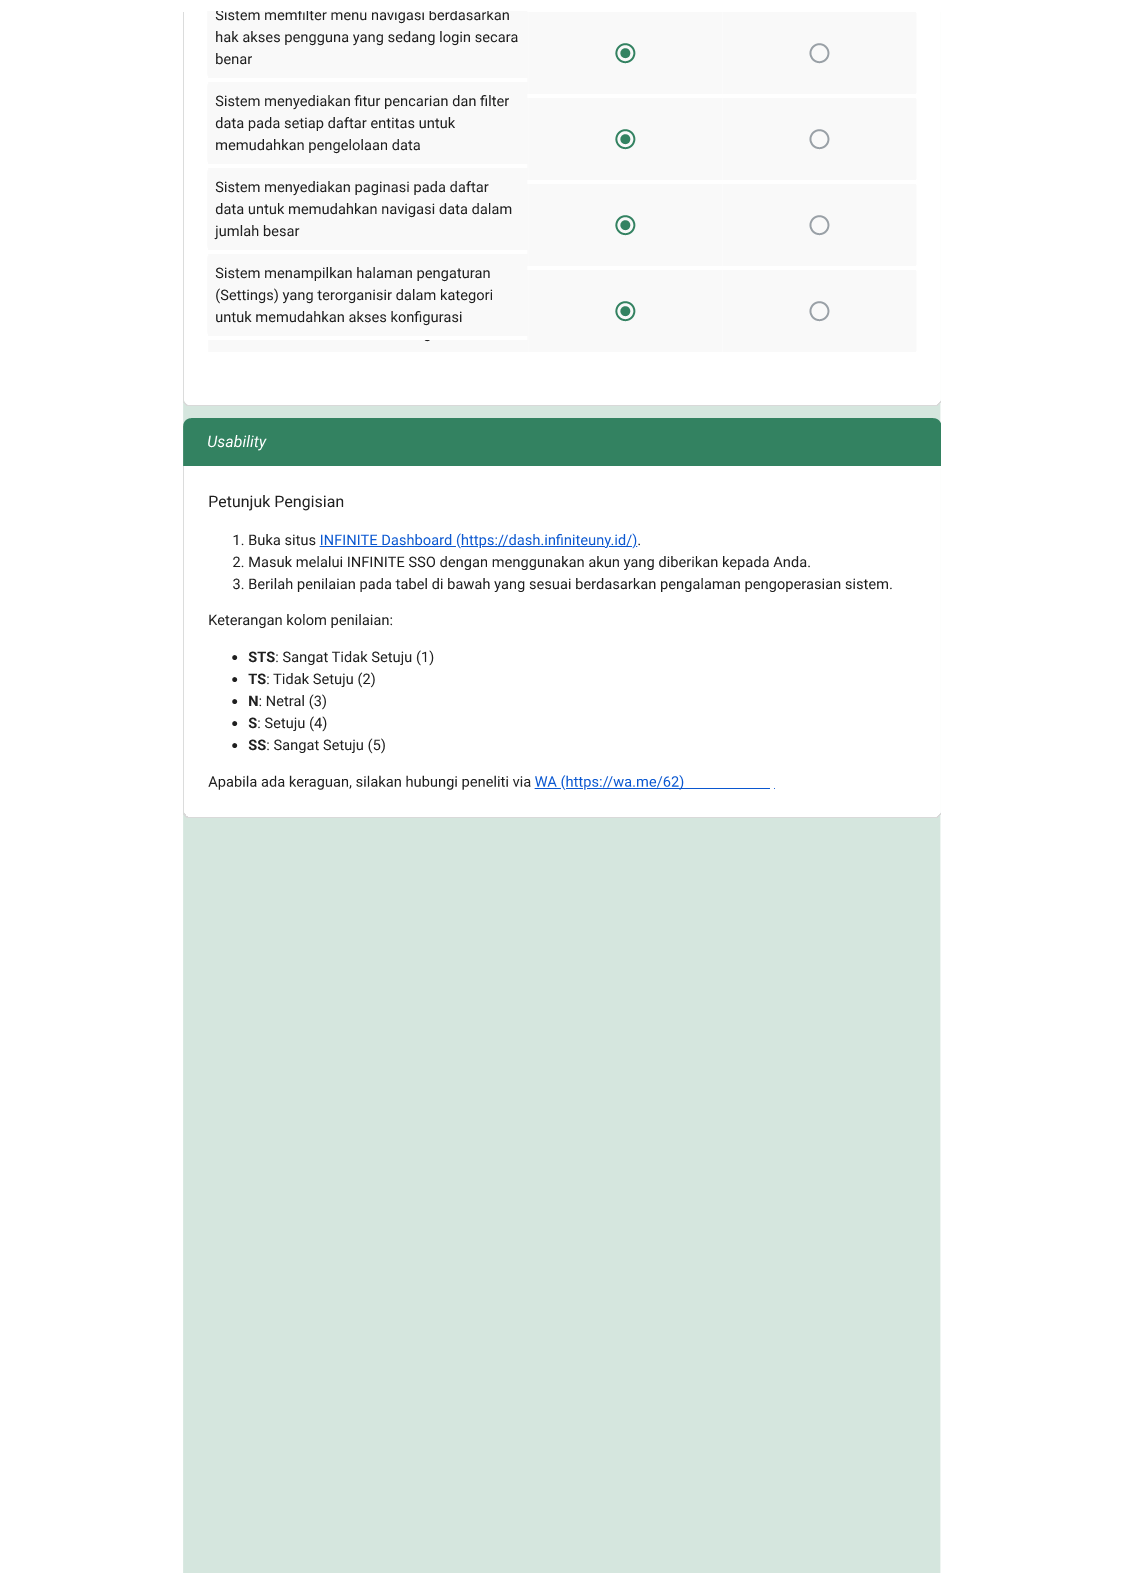
\includegraphics[width=1\textwidth,keepaspectratio]{images/product-quality-tests/hasil-product-quality-penguji-4-3.png}
\end{figure}

\begin{figure}[H]
      \centering
      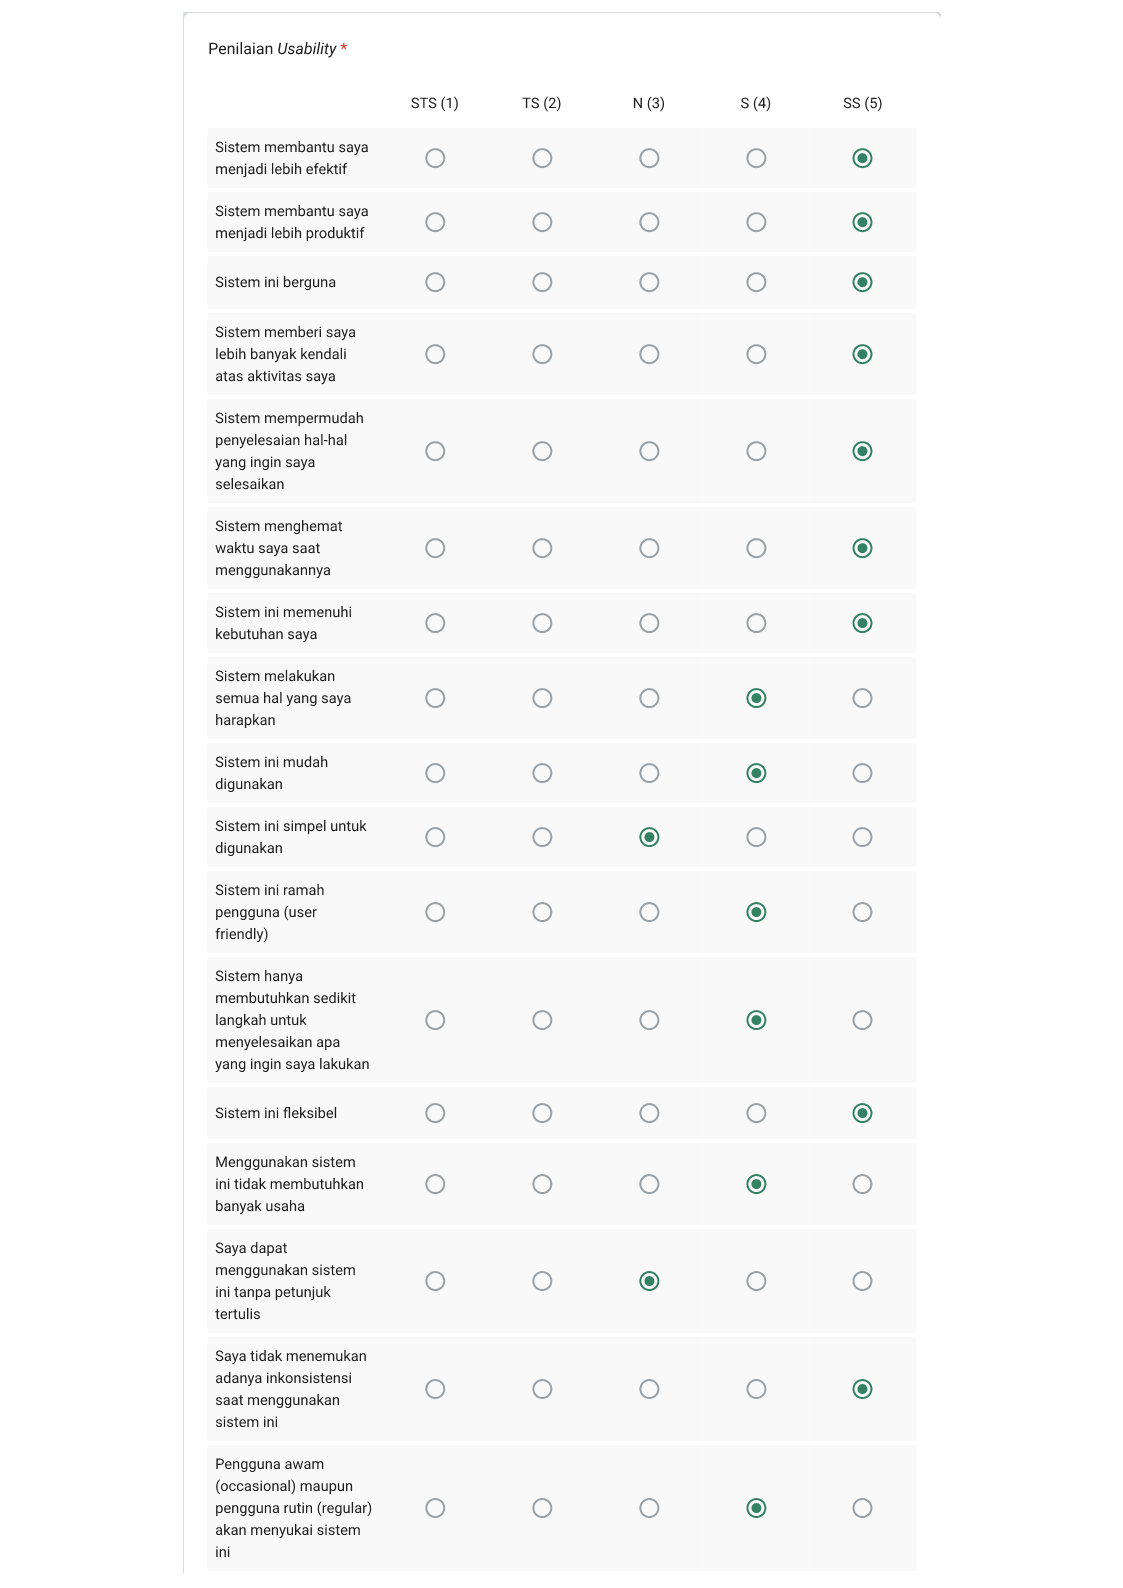
\includegraphics[width=1\textwidth,keepaspectratio]{images/product-quality-tests/hasil-product-quality-penguji-4-4.png}
\end{figure}

\begin{figure}[H]
      \centering
      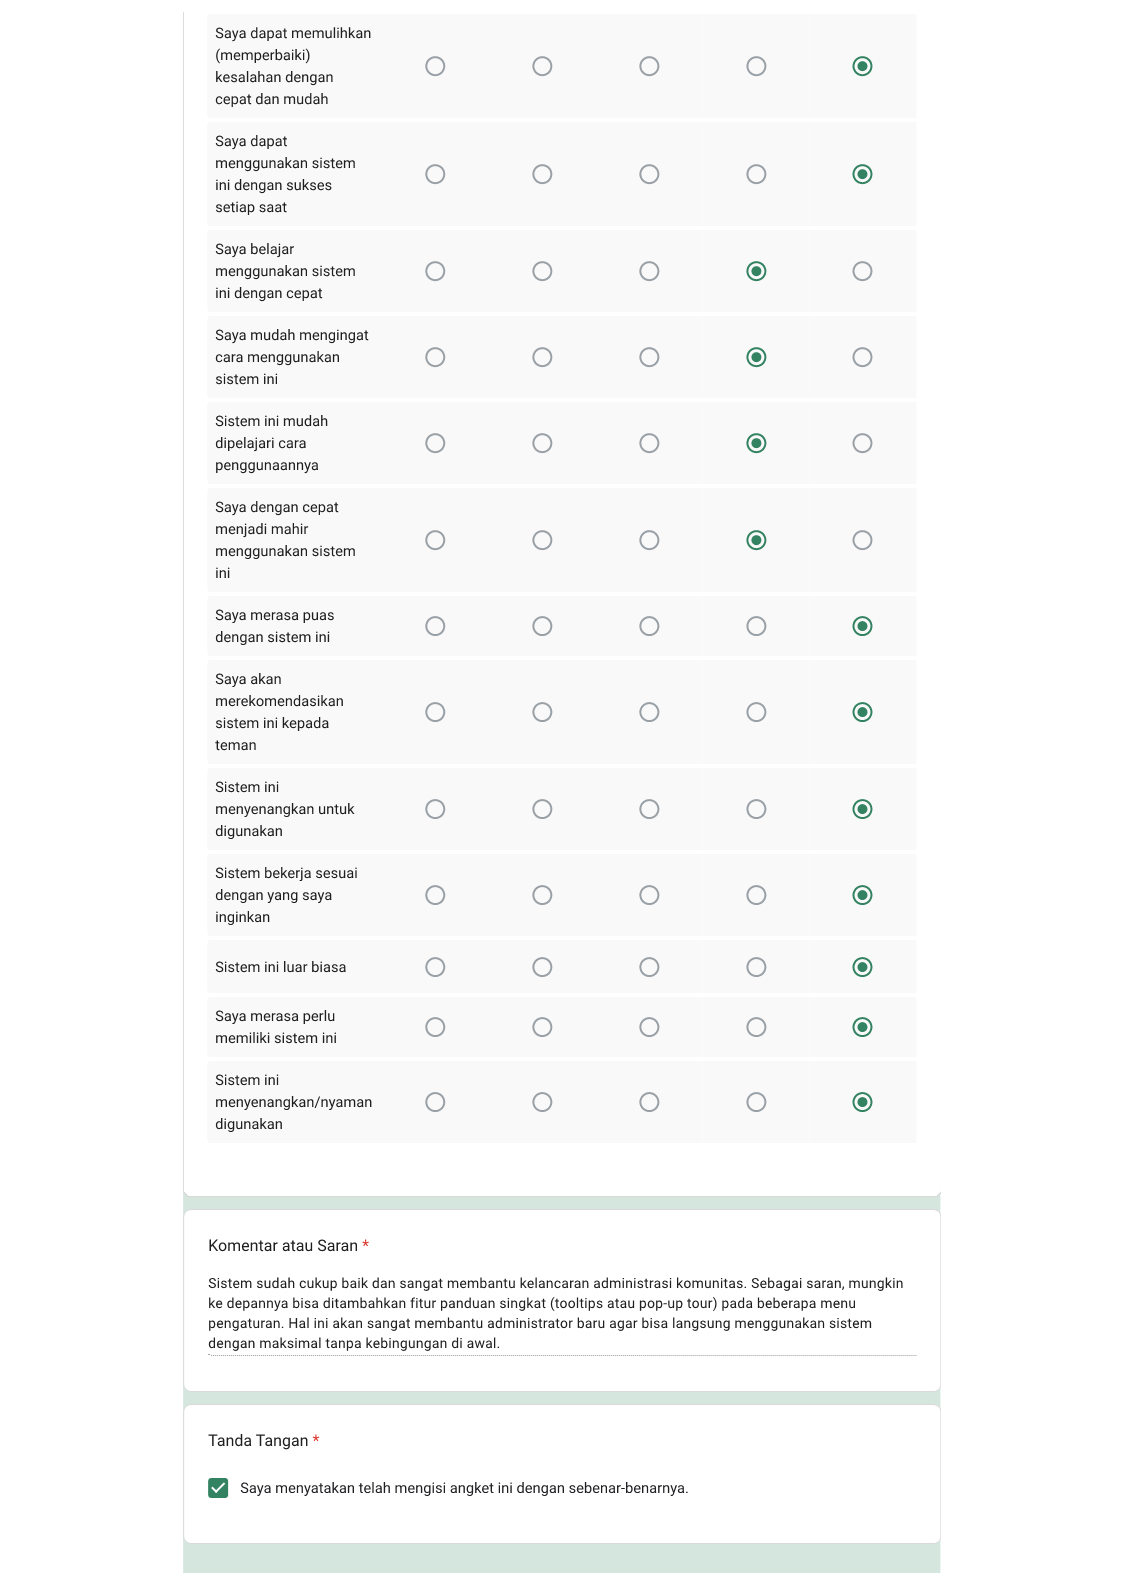
\includegraphics[width=1\textwidth,keepaspectratio]{images/product-quality-tests/hasil-product-quality-penguji-4-5.png}
\end{figure}

\newpage

\noindent Penguji 5

\begin{figure}[H]
      \centering
      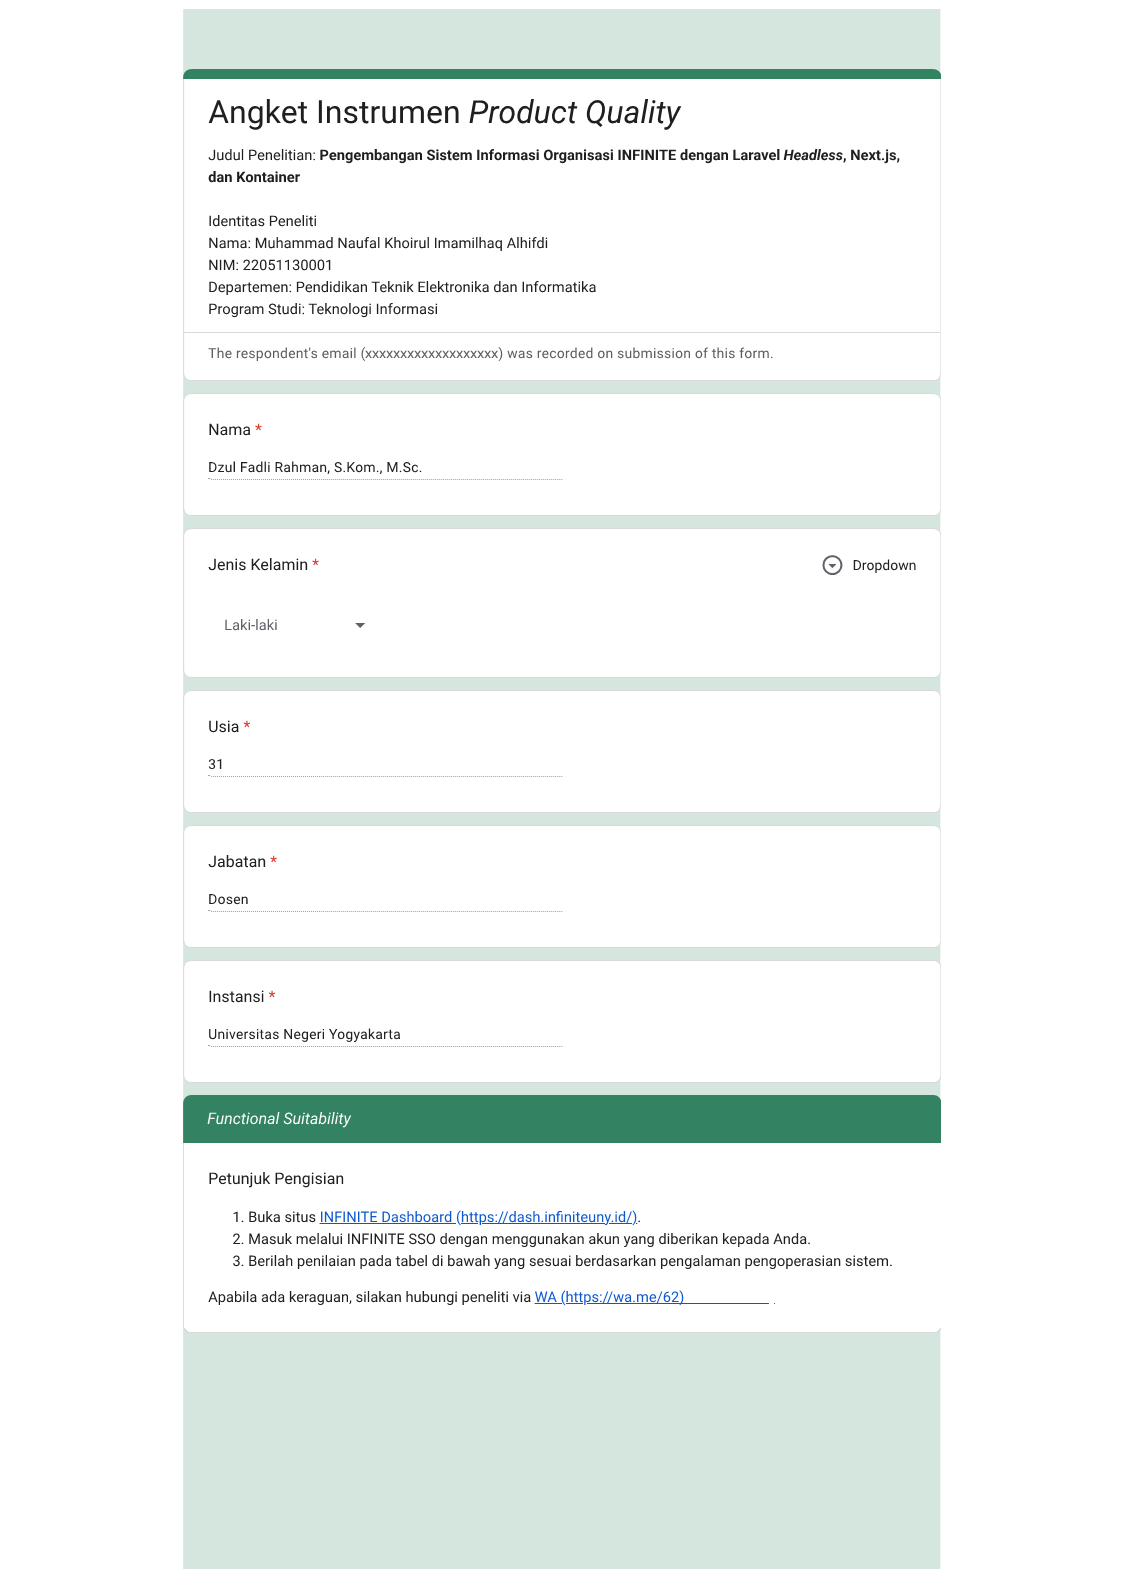
\includegraphics[width=1\textwidth,keepaspectratio]{images/product-quality-tests/hasil-product-quality-penguji-5-1.png}
\end{figure}

\begin{figure}[H]
      \centering
      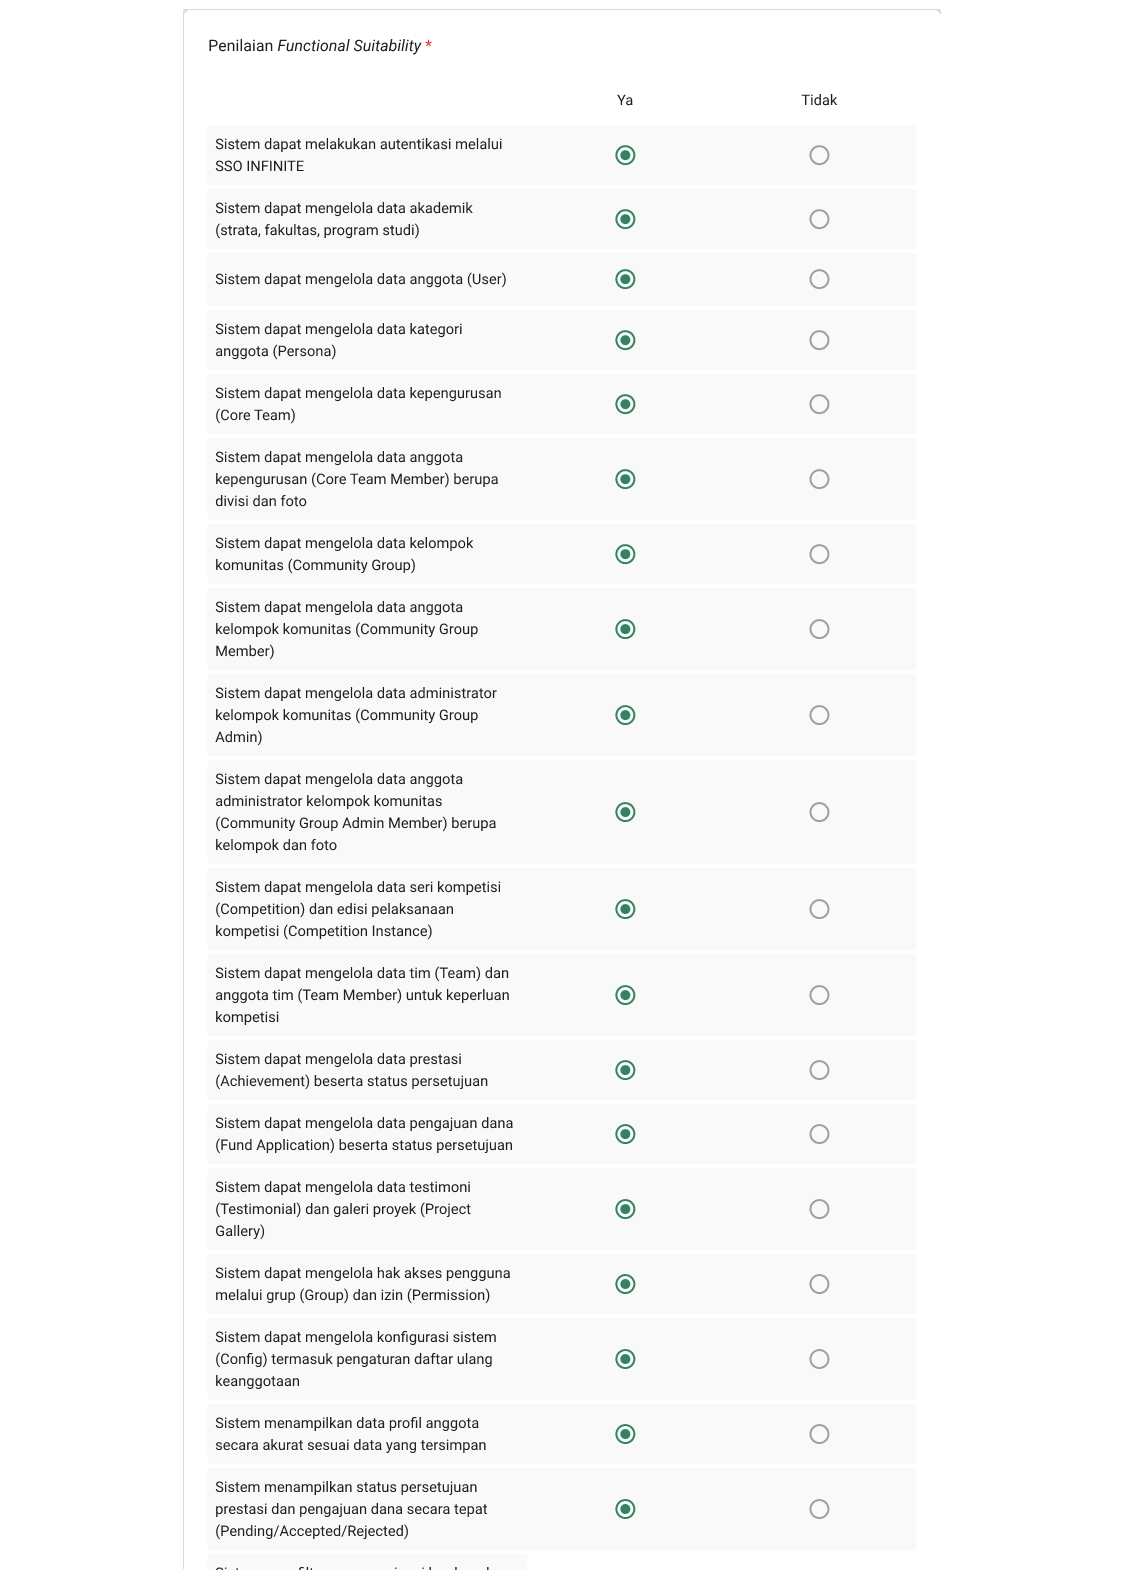
\includegraphics[width=1\textwidth,keepaspectratio]{images/product-quality-tests/hasil-product-quality-penguji-5-2.png}
\end{figure}

\begin{figure}[H]
      \centering
      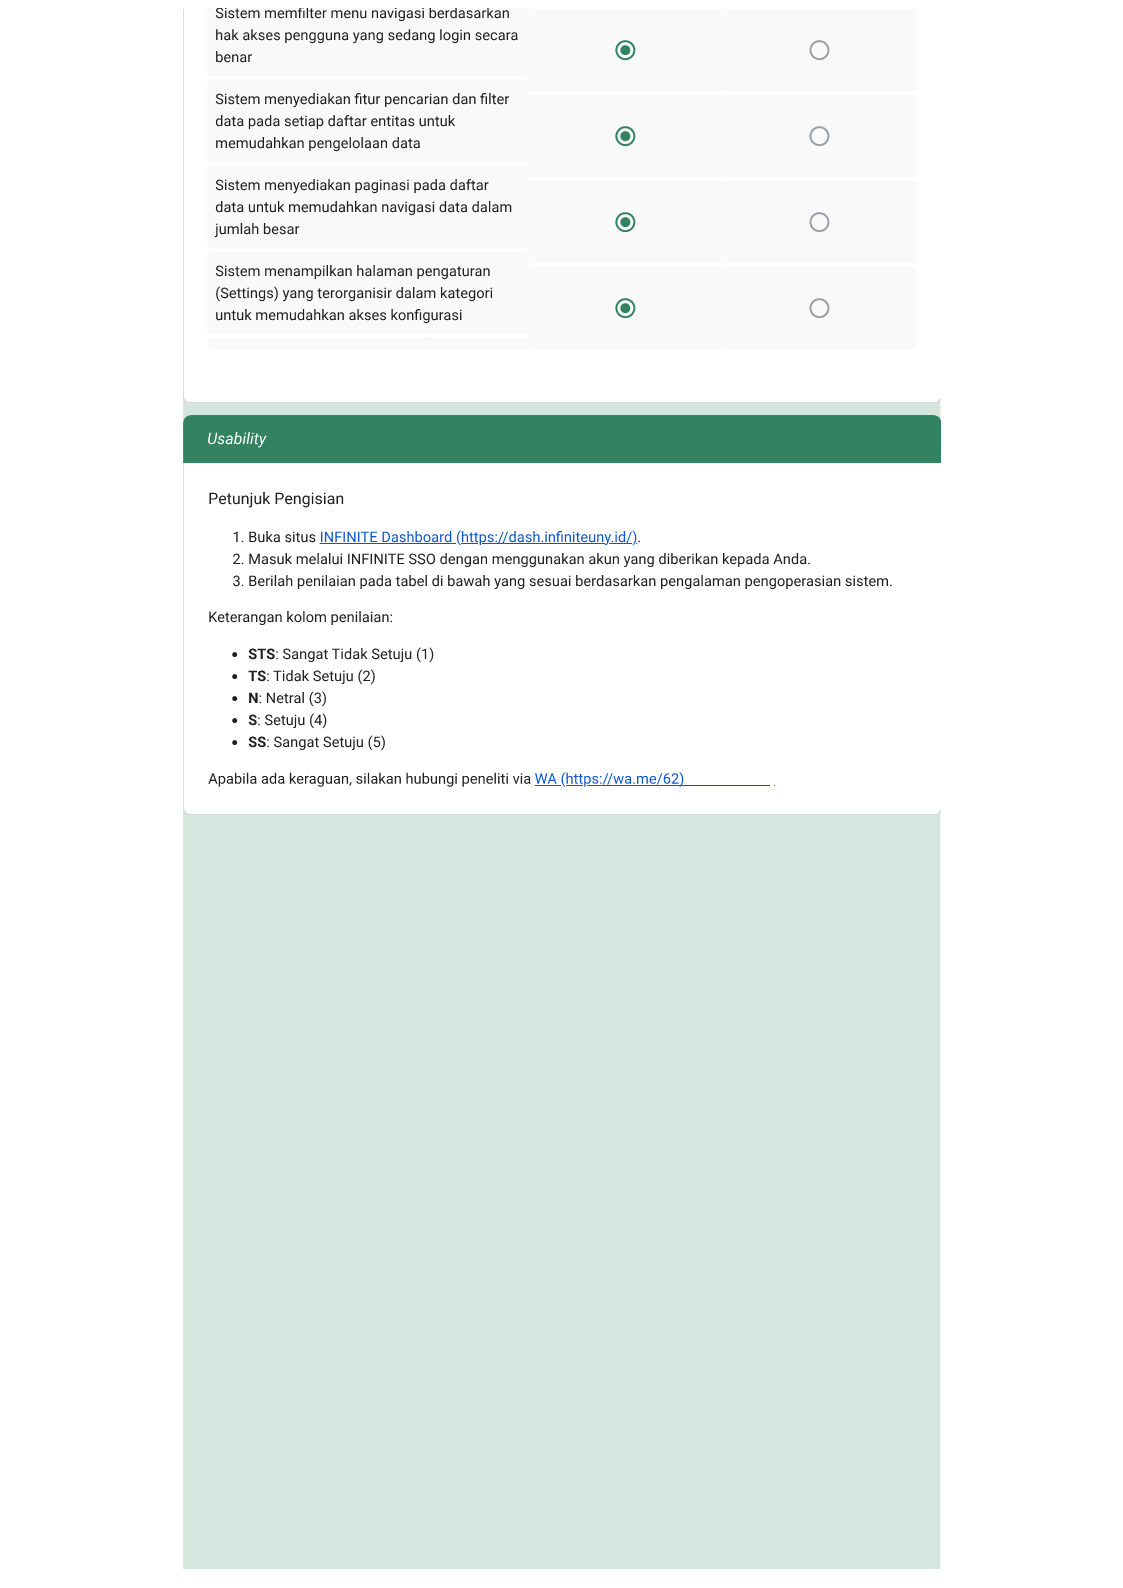
\includegraphics[width=1\textwidth,keepaspectratio]{images/product-quality-tests/hasil-product-quality-penguji-5-3.png}
\end{figure}

\begin{figure}[H]
      \centering
      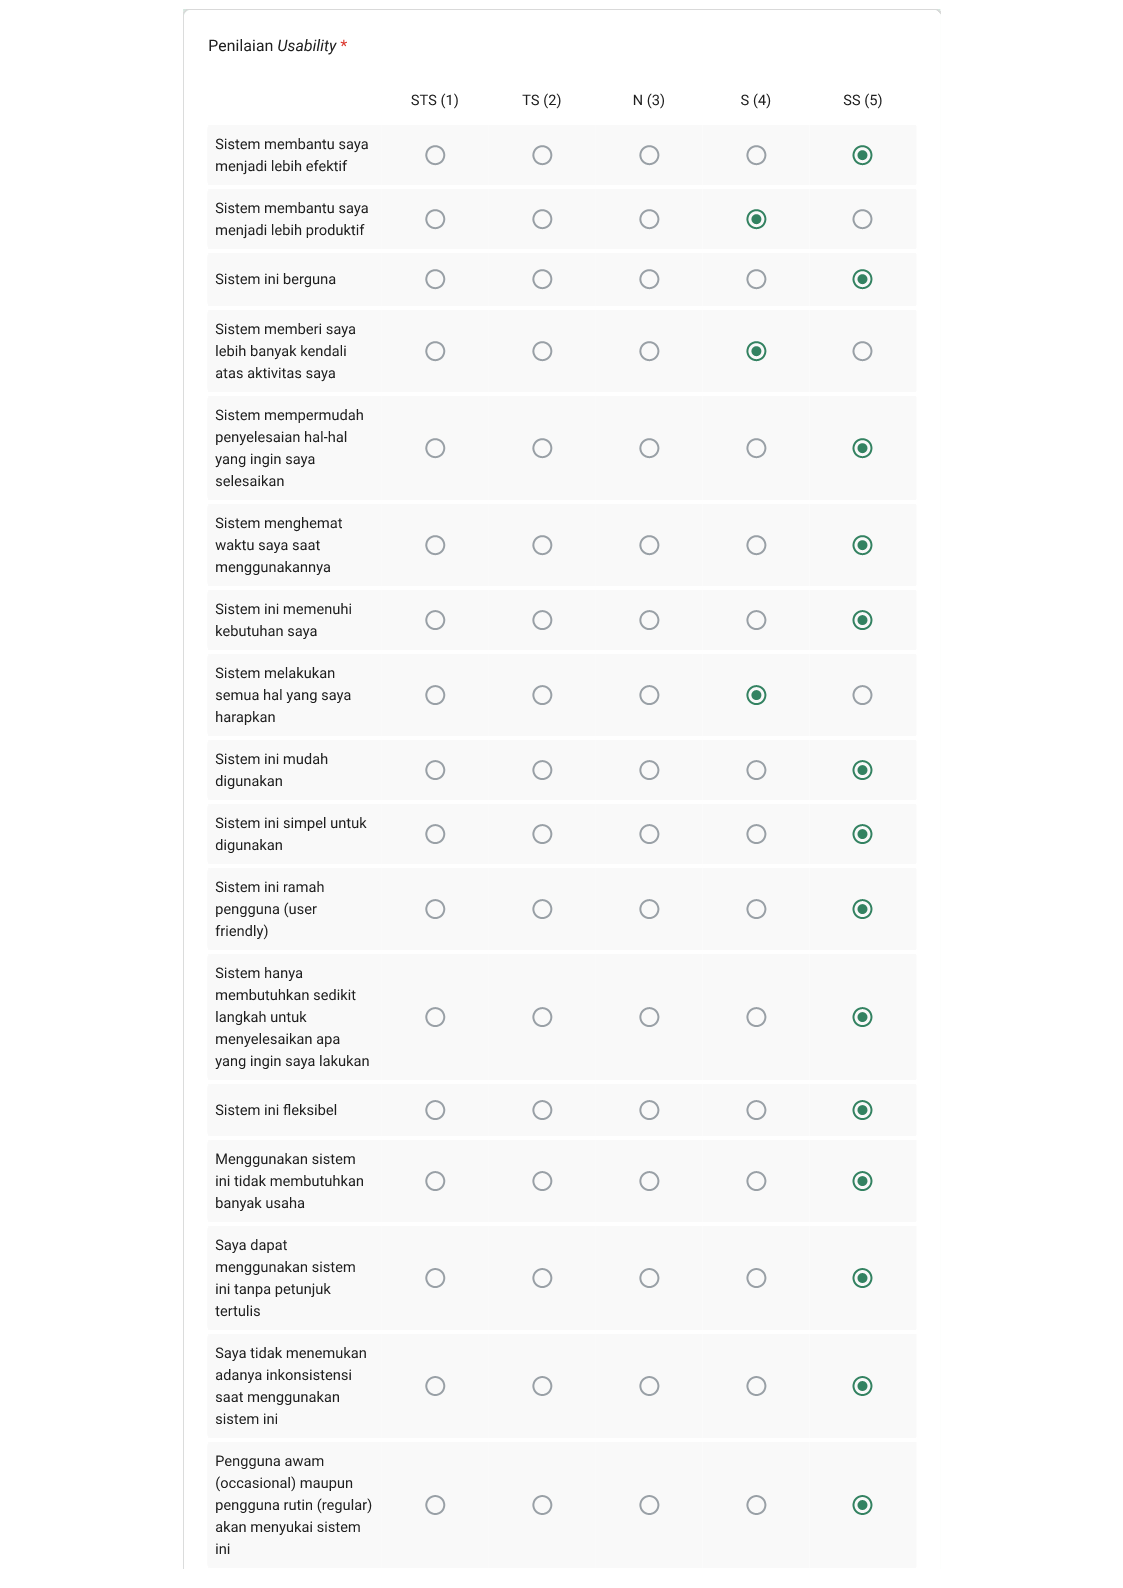
\includegraphics[width=1\textwidth,keepaspectratio]{images/product-quality-tests/hasil-product-quality-penguji-5-4.png}
\end{figure}

\begin{figure}[H]
      \centering
      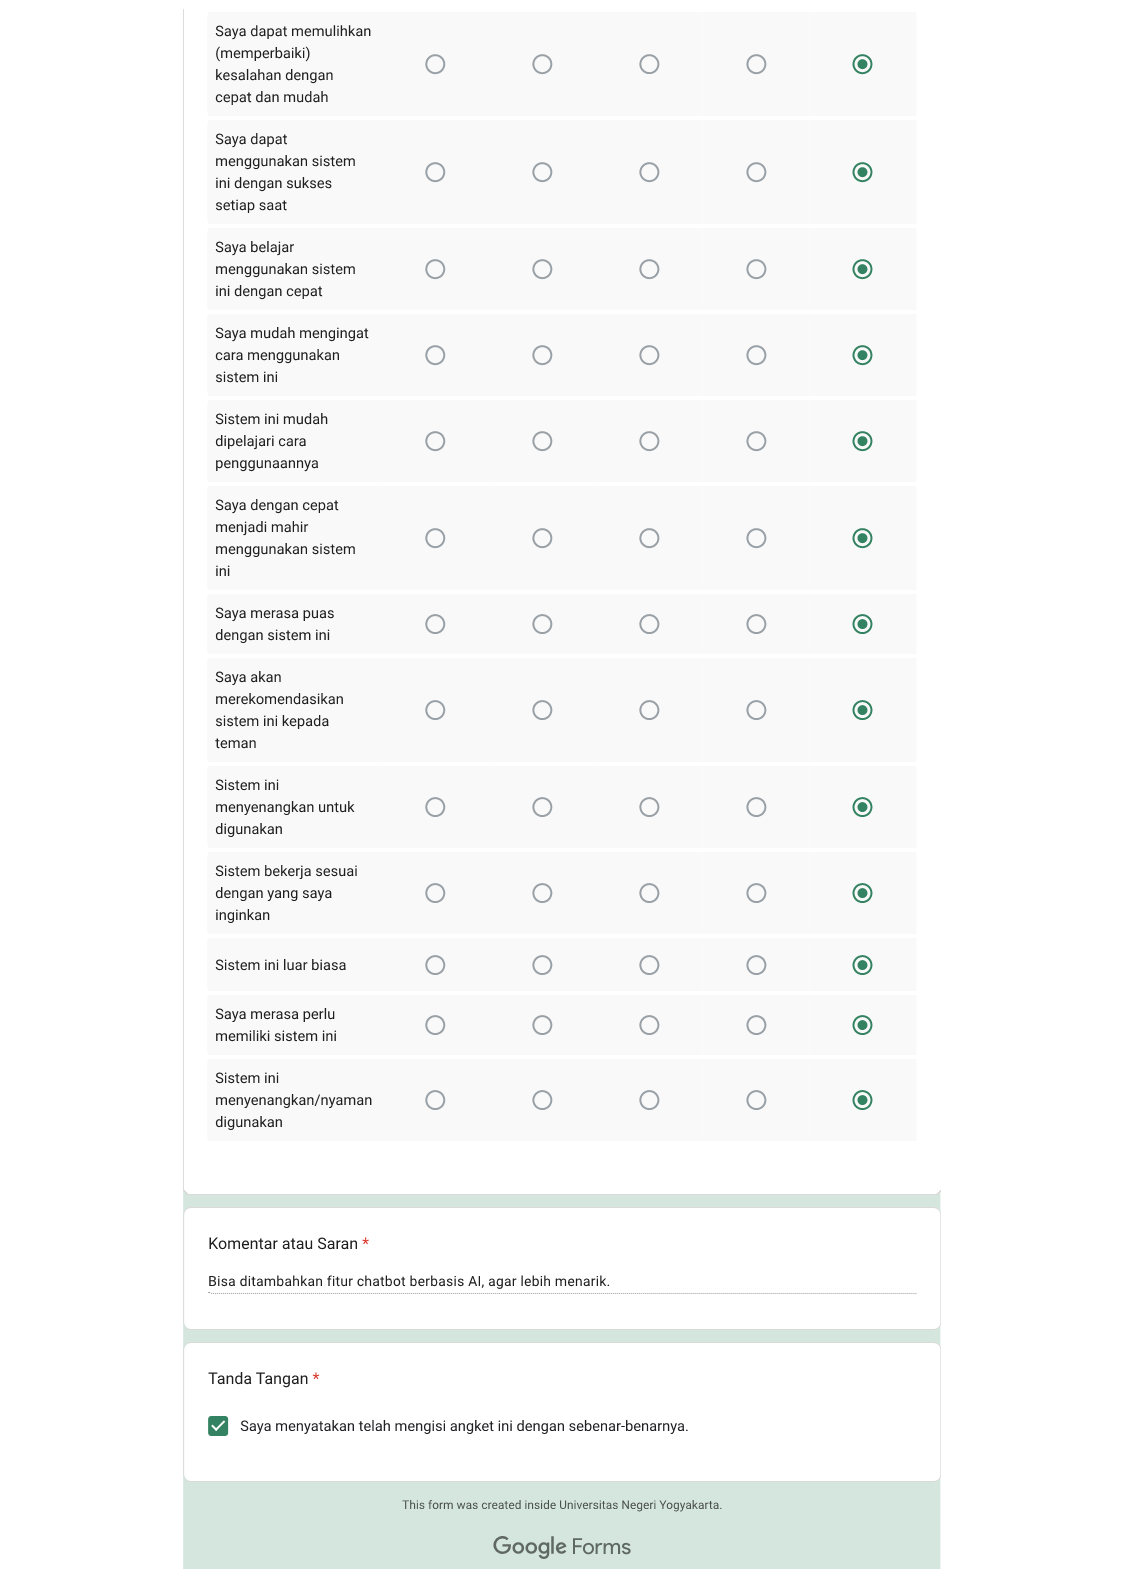
\includegraphics[width=1\textwidth,keepaspectratio]{images/product-quality-tests/hasil-product-quality-penguji-5-5.png}
\end{figure}

\newpage

\annex{Hasil Pengujian \textit{Performance Efficiency Frontend}}
\label{annex:performance-frontend}

\begingroup
\fontsize{9}{11}\selectfont
\begin{longtable}{|c|p{5cm}|c|c|c|c|c|c|}
      \hline
      \textbf{No.}                             & \textbf{URL}                                               & \textbf{FCP}     & \textbf{LCP}     & \textbf{TBT}     & \textbf{CLS}     & \textbf{SI}      & \textbf{Skor} \\
      \hline
      \endfirsthead

      \hline
      \textbf{No.}                             & \textbf{URL}                                               & \textbf{FCP}     & \textbf{LCP}     & \textbf{TBT}     & \textbf{CLS}     & \textbf{SI}      & \textbf{Skor} \\
      \hline
      \endhead

      \hline
      \endfoot

      \hline
      \endlastfoot

      1                                        & \url{/}                                                    & 100              & 95               & 95               & 100              & 40               & 91            \\
      \hline
      2                                        & \url{/achievements}                                        & 100              & 99               & 65               & 100              & 72               & 86            \\
      \hline
      3                                        & \url{/achievements/[id]}                                   & 100              & 100              & 65               & 100              & 83               & 88            \\
      \hline
      4                                        & \url{/achievements/[id]/edit}                              & 100              & 100              & 65               & 100              & 61               & 86            \\
      \hline
      5                                        & \url{/achievements/new}                                    & 100              & 99               & 98               & 100              & 78               & 97            \\
      \hline
      6                                        & \url{/community-group-admins}                              & 99               & 94               & 68               & 100              & 74               & 86            \\
      \hline
      7                                        & \url{/community-group-admins/[id]}                         & 100              & 97               & 73               & 100              & 86               & 90            \\
      \hline
      8                                        & \url{/community-group-admins/[id]/edit}                    & 98               & 96               & 71               & 100              & 77               & 88            \\
      \hline
      9                                        & \url{/community-group-admins/[id]/members}                 & 100              & 99               & 82               & 100              & 75               & 92            \\
      \hline
      10                                       & \url{/community-group-admins/[id]/members/[memberId]}      & 100              & 92               & 67               & 99               & 78               & 86            \\
      \hline
      11                                       & \url{/community-group-admins/[id]/members/[memberId]/edit} & 100              & 53               & 91               & 100              & 70               & 83            \\
      \hline
      12                                       & \url{/community-group-admins/[id]/members/new}             & 100              & 100              & 99               & 100              & 59               & 96            \\
      \hline
      13                                       & \url{/community-group-admins/new}                          & 100              & 100              & 100              & 100              & 94               & 99            \\
      \hline
      14                                       & \url{/community-groups}                                    & 100              & 100              & 42               & 100              & 80               & 81            \\
      \hline
      15                                       & \url{/community-groups/[id]}                               & 99               & 77               & 80               & 100              & 84               & 87            \\
      \hline
      16                                       & \url{/community-groups/[id]/edit}                          & 99               & 85               & 67               & 99               & 63               & 82            \\
      \hline
      17                                       & \url{/community-groups/[id]/members}                       & 100              & 98               & 66               & 100              & 73               & 87            \\
      \hline
      18                                       & \url{/community-groups/[id]/members/new}                   & 100              & 100              & 49               & 100              & 71               & 82            \\
      \hline
      19                                       & \url{/community-groups/new}                                & 100              & 94               & 100              & 100              & 91               & 98            \\
      \hline
      20                                       & \url{/competition-organizer-types}                         & 100              & 93               & 100              & 100              & 76               & 96            \\
      \hline
      21                                       & \url{/competition-organizer-types/[id]}                    & 99               & 88               & 62               & 100              & 77               & 83            \\
      \hline
      22                                       & \url{/competition-organizer-types/[id]/edit}               & 100              & 98               & 100              & 100              & 87               & 98            \\
      \hline
      23                                       & \url{/competition-organizer-types/new}                     & 100              & 96               & 100              & 100              & 91               & 98            \\
      \hline
      24                                       & \url{/competition-outputs}                                 & 98               & 99               & 74               & 100              & 74               & 89            \\
      \hline
      25                                       & \url{/competition-outputs/[id]}                            & 99               & 88               & 58               & 100              & 76               & 82            \\
      \hline
      26                                       & \url{/competition-outputs/[id]/edit}                       & 100              & 100              & 47               & 100              & 67               & 81            \\
      \hline
      27                                       & \url{/competition-outputs/new}                             & 100              & 91               & 99               & 100              & 88               & 96            \\
      \hline
      28                                       & \url{/competition-ranks}                                   & 99               & 99               & 55               & 100              & 66               & 83            \\
      \hline
      29                                       & \url{/competition-ranks/[id]}                              & 99               & 84               & 71               & 100              & 73               & 84            \\
      \hline
      30                                       & \url{/competition-ranks/[id]/edit}                         & 69               & 87               & 88               & 100              & 44               & 84            \\
      \hline
      31                                       & \url{/competition-ranks/new}                               & 100              & 99               & 100              & 100              & 95               & 99            \\
      \hline
      32                                       & \url{/competition-scales}                                  & 99               & 91               & 63               & 100              & 62               & 83            \\
      \hline
      33                                       & \url{/competition-scales/[id]}                             & 98               & 93               & 61               & 100              & 61               & 82            \\
      \hline
      34                                       & \url{/competition-scales/[id]/edit}                        & 98               & 94               & 58               & 100              & 66               & 82            \\
      \hline
      35                                       & \url{/competition-scales/new}                              & 100              & 94               & 100              & 100              & 93               & 98            \\
      \hline
      36                                       & \url{/competition-time-ranges}                             & 99               & 89               & 67               & 100              & 63               & 84            \\
      \hline
      37                                       & \url{/competition-time-ranges/[id]}                        & 100              & 100              & 44               & 100              & 83               & 82            \\
      \hline
      38                                       & \url{/competition-time-ranges/[id]/edit}                   & 99               & 99               & 47               & 100              & 69               & 81            \\
      \hline
      39                                       & \url{/competition-time-ranges/new}                         & 100              & 96               & 100              & 100              & 95               & 99            \\
      \hline
      40                                       & \url{/competitions}                                        & 100              & 75               & 75               & 100              & 66               & 83            \\
      \hline
      41                                       & \url{/competitions/[id]}                                   & 100              & 98               & 48               & 100              & 70               & 81            \\
      \hline
      42                                       & \url{/competitions/[id]/edit}                              & 100              & 100              & 57               & 100              & 82               & 85            \\
      \hline
      43                                       & \url{/competitions/[id]/instances}                         & 100              & 92               & 97               & 100              & 72               & 94            \\
      \hline
      44                                       & \url{/competitions/[id]/instances/[instanceId]}            & 100              & 99               & 69               & 100              & 86               & 89            \\
      \hline
      45                                       & \url{/competitions/[id]/instances/[instanceId]/edit}       & 100              & 68               & 100              & 100              & 66               & 89            \\
      \hline
      46                                       & \url{/competitions/[id]/instances/new}                     & 100              & 95               & 100              & 100              & 78               & 97            \\
      \hline
      47                                       & \url{/competitions/new}                                    & 100              & 100              & 100              & 100              & 93               & 99            \\
      \hline
      48                                       & \url{/core-team-divisions}                                 & 100              & 76               & 82               & 100              & 73               & 86            \\
      \hline
      49                                       & \url{/core-team-divisions/[id]}                            & 100              & 98               & 60               & 100              & 75               & 85            \\
      \hline
      50                                       & \url{/core-team-divisions/[id]/edit}                       & 100              & 99               & 58               & 100              & 82               & 85            \\
      \hline
      51                                       & \url{/core-team-divisions/new}                             & 100              & 99               & 100              & 100              & 95               & 99            \\
      \hline
      52                                       & \url{/core-teams}                                          & 100              & 98               & 72               & 100              & 79               & 89            \\
      \hline
      53                                       & \url{/core-teams/[id]}                                     & 100              & 99               & 57               & 100              & 76               & 84            \\
      \hline
      54                                       & \url{/core-teams/[id]/edit}                                & 100              & 97               & 58               & 100              & 77               & 84            \\
      \hline
      55                                       & \url{/core-teams/[id]/members}                             & 100              & 100              & 55               & 100              & 68               & 83            \\
      \hline
      56                                       & \url{/core-teams/[id]/members/[memberId]}                  & 100              & 89               & 57               & 99               & 67               & 81            \\
      \hline
      57                                       & \url{/core-teams/[id]/members/[memberId]/edit}             & 100              & 72               & 100              & 98               & 83               & 91            \\
      \hline
      58                                       & \url{/core-teams/[id]/members/new}                         & 100              & 98               & 100              & 100              & 68               & 96            \\
      \hline
      59                                       & \url{/core-teams/new}                                      & 100              & 100              & 100              & 100              & 81               & 98            \\
      \hline
      60                                       & \url{/degrees}                                             & 100              & 99               & 59               & 100              & 68               & 84            \\
      \hline
      61                                       & \url{/degrees/[id]}                                        & 100              & 99               & 76               & 100              & 83               & 91            \\
      \hline
      62                                       & \url{/degrees/[id]/edit}                                   & 100              & 100              & 64               & 100              & 80               & 87            \\
      \hline
      63                                       & \url{/degrees/new}                                         & 100              & 95               & 100              & 100              & 94               & 98            \\
      \hline
      64                                       & \url{/faculties}                                           & 100              & 83               & 66               & 100              & 66               & 82            \\
      \hline
      65                                       & \url{/faculties/[id]}                                      & 100              & 78               & 63               & 100              & 77               & 81            \\
      \hline
      66                                       & \url{/faculties/[id]/edit}                                 & 100              & 99               & 63               & 100              & 81               & 87            \\
      \hline
      67                                       & \url{/faculties/new}                                       & 100              & 93               & 100              & 100              & 94               & 98            \\
      \hline
      68                                       & \url{/fund-applications}                                   & 100              & 98               & 54               & 100              & 63               & 82            \\
      \hline
      69                                       & \url{/fund-applications/[id]}                              & 100              & 100              & 62               & 100              & 73               & 86            \\
      \hline
      70                                       & \url{/fund-applications/[id]/edit}                         & 100              & 100              & 54               & 100              & 45               & 81            \\
      \hline
      71                                       & \url{/fund-applications/new}                               & 100              & 99               & 100              & 100              & 77               & 97            \\
      \hline
      72                                       & \url{/groups}                                              & 88               & 92               & 90               & 100              & 48               & 89            \\
      \hline
      73                                       & \url{/groups/[id]}                                         & 100              & 100              & 57               & 100              & 56               & 83            \\
      \hline
      74                                       & \url{/groups/[id]/edit}                                    & 100              & 90               & 100              & 100              & 93               & 97            \\
      \hline
      75                                       & \url{/groups/[id]/permissions}                             & 100              & 100              & 67               & 100              & 74               & 88            \\
      \hline
      76                                       & \url{/groups/[id]/permissions/new}                         & 100              & 100              & 83               & 100              & 76               & 93            \\
      \hline
      77                                       & \url{/groups/new}                                          & 95               & 98               & 100              & 100              & 72               & 96            \\
      \hline
      78                                       & \url{/login}                                               & 100              & 99               & 78               & 100              & 84               & 92            \\
      \hline
      79                                       & \url{/majors}                                              & 100              & 94               & 100              & 100              & 78               & 96            \\
      \hline
      80                                       & \url{/majors/[id]}                                         & 100              & 100              & 76               & 100              & 80               & 91            \\
      \hline
      81                                       & \url{/majors/[id]/edit}                                    & 100              & 100              & 68               & 100              & 71               & 88            \\
      \hline
      82                                       & \url{/majors/new}                                          & 100              & 91               & 100              & 100              & 91               & 97            \\
      \hline
      83                                       & \url{/permissions}                                         & 100              & 100              & 80               & 99               & 52               & 89            \\
      \hline
      84                                       & \url{/permissions/[id]}                                    & 100              & 100              & 57               & 100              & 81               & 85            \\
      \hline
      85                                       & \url{/permissions/[id]/edit}                               & 100              & 100              & 71               & 100              & 85               & 90            \\
      \hline
      86                                       & \url{/permissions/new}                                     & 100              & 91               & 100              & 100              & 92               & 97            \\
      \hline
      87                                       & \url{/personas}                                            & 100              & 89               & 62               & 100              & 83               & 84            \\
      \hline
      88                                       & \url{/personas/[id]}                                       & 100              & 95               & 66               & 100              & 79               & 86            \\
      \hline
      89                                       & \url{/personas/[id]/edit}                                  & 100              & 78               & 74               & 100              & 74               & 84            \\
      \hline
      90                                       & \url{/personas/new}                                        & 100              & 94               & 100              & 100              & 92               & 98            \\
      \hline
      91                                       & \url{/project-galleries}                                   & 100              & 100              & 61               & 100              & 85               & 87            \\
      \hline
      92                                       & \url{/project-galleries/[id]}                              & 100              & 96               & 71               & 99               & 80               & 88            \\
      \hline
      93                                       & \url{/project-galleries/[id]/edit}                         & 100              & 79               & 72               & 100              & 51               & 81            \\
      \hline
      94                                       & \url{/project-galleries/new}                               & 100              & 98               & 100              & 100              & 85               & 98            \\
      \hline
      95                                       & \url{/settings}                                            & 100              & 99               & 63               & 100              & 82               & 87            \\
      \hline
      96                                       & \url{/settings/profile}                                    & 99               & 97               & 78               & 100              & 67               & 89            \\
      \hline
      97                                       & \url{/settings/profile/community-groups}                   & 100              & 99               & 85               & 100              & 83               & 94            \\
      \hline
      98                                       & \url{/settings/profile/community-groups/new}               & 100              & 99               & 100              & 100              & 90               & 99            \\
      \hline
      99                                       & \url{/settings/profile/edit}                               & 100              & 100              & 65               & 100              & 70               & 87            \\
      \hline
      100                                      & \url{/settings/profile/groups}                             & 100              & 99               & 95               & 100              & 84               & 97            \\
      \hline
      101                                      & \url{/settings/profile/groups/new}                         & 100              & 99               & 100              & 100              & 89               & 99            \\
      \hline
      102                                      & \url{/settings/profile/permissions}                        & 100              & 98               & 97               & 100              & 83               & 97            \\
      \hline
      103                                      & \url{/settings/profile/permissions/new}                    & 100              & 94               & 99               & 100              & 89               & 97            \\
      \hline
      104                                      & \url{/settings/profile/personas}                           & 100              & 72               & 89               & 100              & 72               & 87            \\
      \hline
      105                                      & \url{/settings/profile/personas/new}                       & 100              & 89               & 99               & 100              & 82               & 95            \\
      \hline
      106                                      & \url{/settings/reregistration}                             & 100              & 85               & 91               & 100              & 84               & 92            \\
      \hline
      107                                      & \url{/settings/system}                                     & 100              & 94               & 100              & 100              & 84               & 97            \\
      \hline
      108                                      & \url{/team-types}                                          & 100              & 90               & 93               & 100              & 67               & 92            \\
      \hline
      109                                      & \url{/team-types/[id]}                                     & 100              & 86               & 100              & 100              & 89               & 95            \\
      \hline
      110                                      & \url{/team-types/[id]/edit}                                & 100              & 96               & 100              & 100              & 90               & 98            \\
      \hline
      111                                      & \url{/team-types/new}                                      & 100              & 94               & 100              & 100              & 93               & 98            \\
      \hline
      112                                      & \url{/teams}                                               & 100              & 97               & 91               & 100              & 87               & 95            \\
      \hline
      113                                      & \url{/teams/[id]}                                          & 100              & 99               & 88               & 100              & 85               & 95            \\
      \hline
      114                                      & \url{/teams/[id]/edit}                                     & 100              & 96               & 94               & 100              & 71               & 94            \\
      \hline
      115                                      & \url{/teams/[id]/members}                                  & 100              & 90               & 97               & 100              & 79               & 95            \\
      \hline
      116                                      & \url{/teams/[id]/members/new}                              & 100              & 99               & 96               & 100              & 86               & 97            \\
      \hline
      117                                      & \url{/teams/new}                                           & 100              & 94               & 100              & 100              & 82               & 97            \\
      \hline
      118                                      & \url{/testimonials}                                        & 100              & 89               & 93               & 100              & 77               & 93            \\
      \hline
      119                                      & \url{/testimonials/[id]}                                   & 100              & 66               & 99               & 99               & 78               & 89            \\
      \hline
      120                                      & \url{/testimonials/[id]/edit}                              & 100              & 83               & 95               & 100              & 82               & 92            \\
      \hline
      121                                      & \url{/testimonials/new}                                    & 100              & 84               & 100              & 100              & 93               & 95            \\
      \hline
      122                                      & \url{/users}                                               & 100              & 99               & 57               & 99               & 71               & 84            \\
      \hline
      123                                      & \url{/users/[id]}                                          & 100              & 97               & 87               & 100              & 68               & 92            \\
      \hline
      124                                      & \url{/users/[id]/community-groups}                         & 100              & 94               & 97               & 100              & 75               & 95            \\
      \hline
      125                                      & \url{/users/[id]/community-groups/new}                     & 100              & 99               & 95               & 100              & 76               & 96            \\
      \hline
      126                                      & \url{/users/[id]/edit}                                     & 100              & 99               & 97               & 100              & 66               & 95            \\
      \hline
      127                                      & \url{/users/[id]/groups}                                   & 100              & 99               & 91               & 100              & 82               & 95            \\
      \hline
      128                                      & \url{/users/[id]/groups/new}                               & 100              & 91               & 98               & 100              & 76               & 95            \\
      \hline
      129                                      & \url{/users/[id]/permissions}                              & 100              & 90               & 97               & 100              & 67               & 93            \\
      \hline
      130                                      & \url{/users/[id]/permissions/new}                          & 100              & 90               & 97               & 100              & 82               & 95            \\
      \hline
      131                                      & \url{/users/[id]/personas}                                 & 100              & 99               & 86               & 100              & 79               & 93            \\
      \hline
      132                                      & \url{/users/[id]/personas/new}                             & 100              & 99               & 99               & 100              & 87               & 98            \\
      \hline
      133                                      & \url{/users/new}                                           & 98               & 99               & 100              & 100              & 57               & 95            \\
      \hline
      \multicolumn{2}{|c|}{\textbf{Rata-rata}} & \textbf{99{,}48}                                           & \textbf{93{,}81} & \textbf{81{,}08} & \textbf{99{,}93} & \textbf{76{,}83} & \textbf{90{,}42}                 \\
      \hline
\end{longtable}
\endgroup

\annex{Hasil Pengujian \textit{Performance Efficiency Backend}}
\label{annex:performance-backend}

\begin{figure}[H]
      \centering
      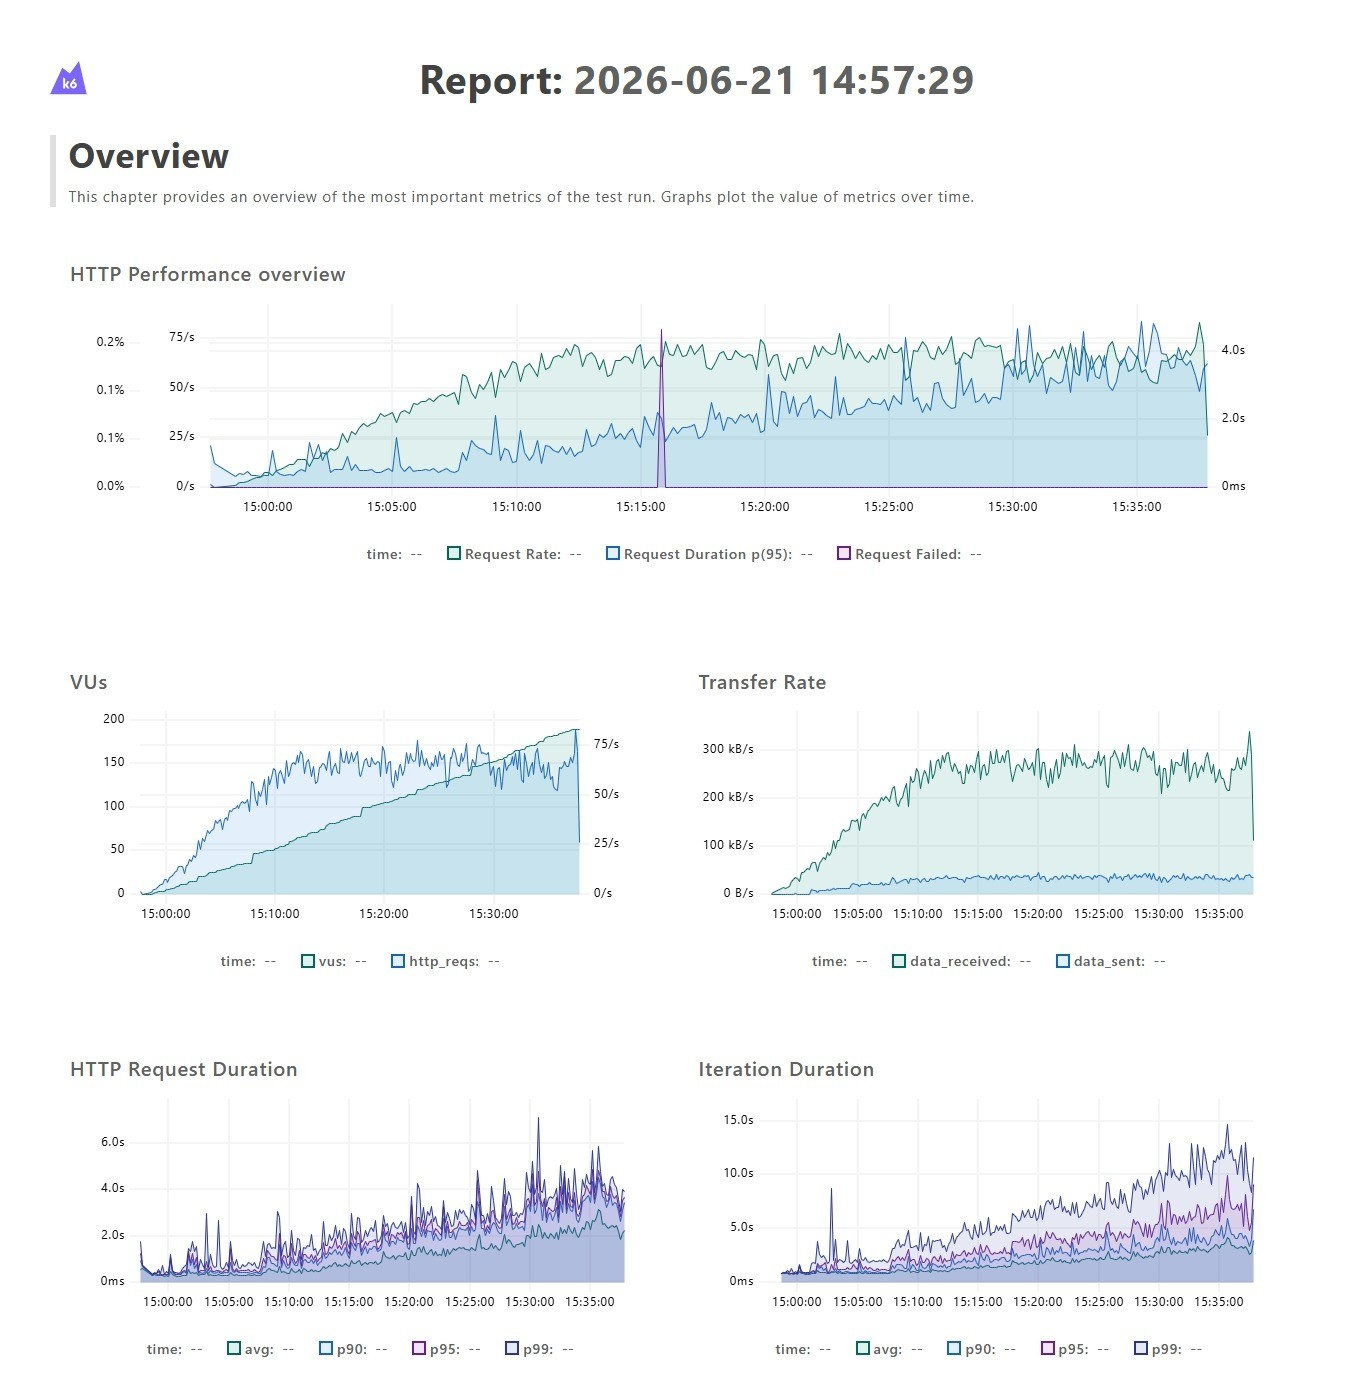
\includegraphics[width=1\textwidth,keepaspectratio]{images/k6-result-overview.jpeg}
\end{figure}

\begin{figure}[H]
      \centering
      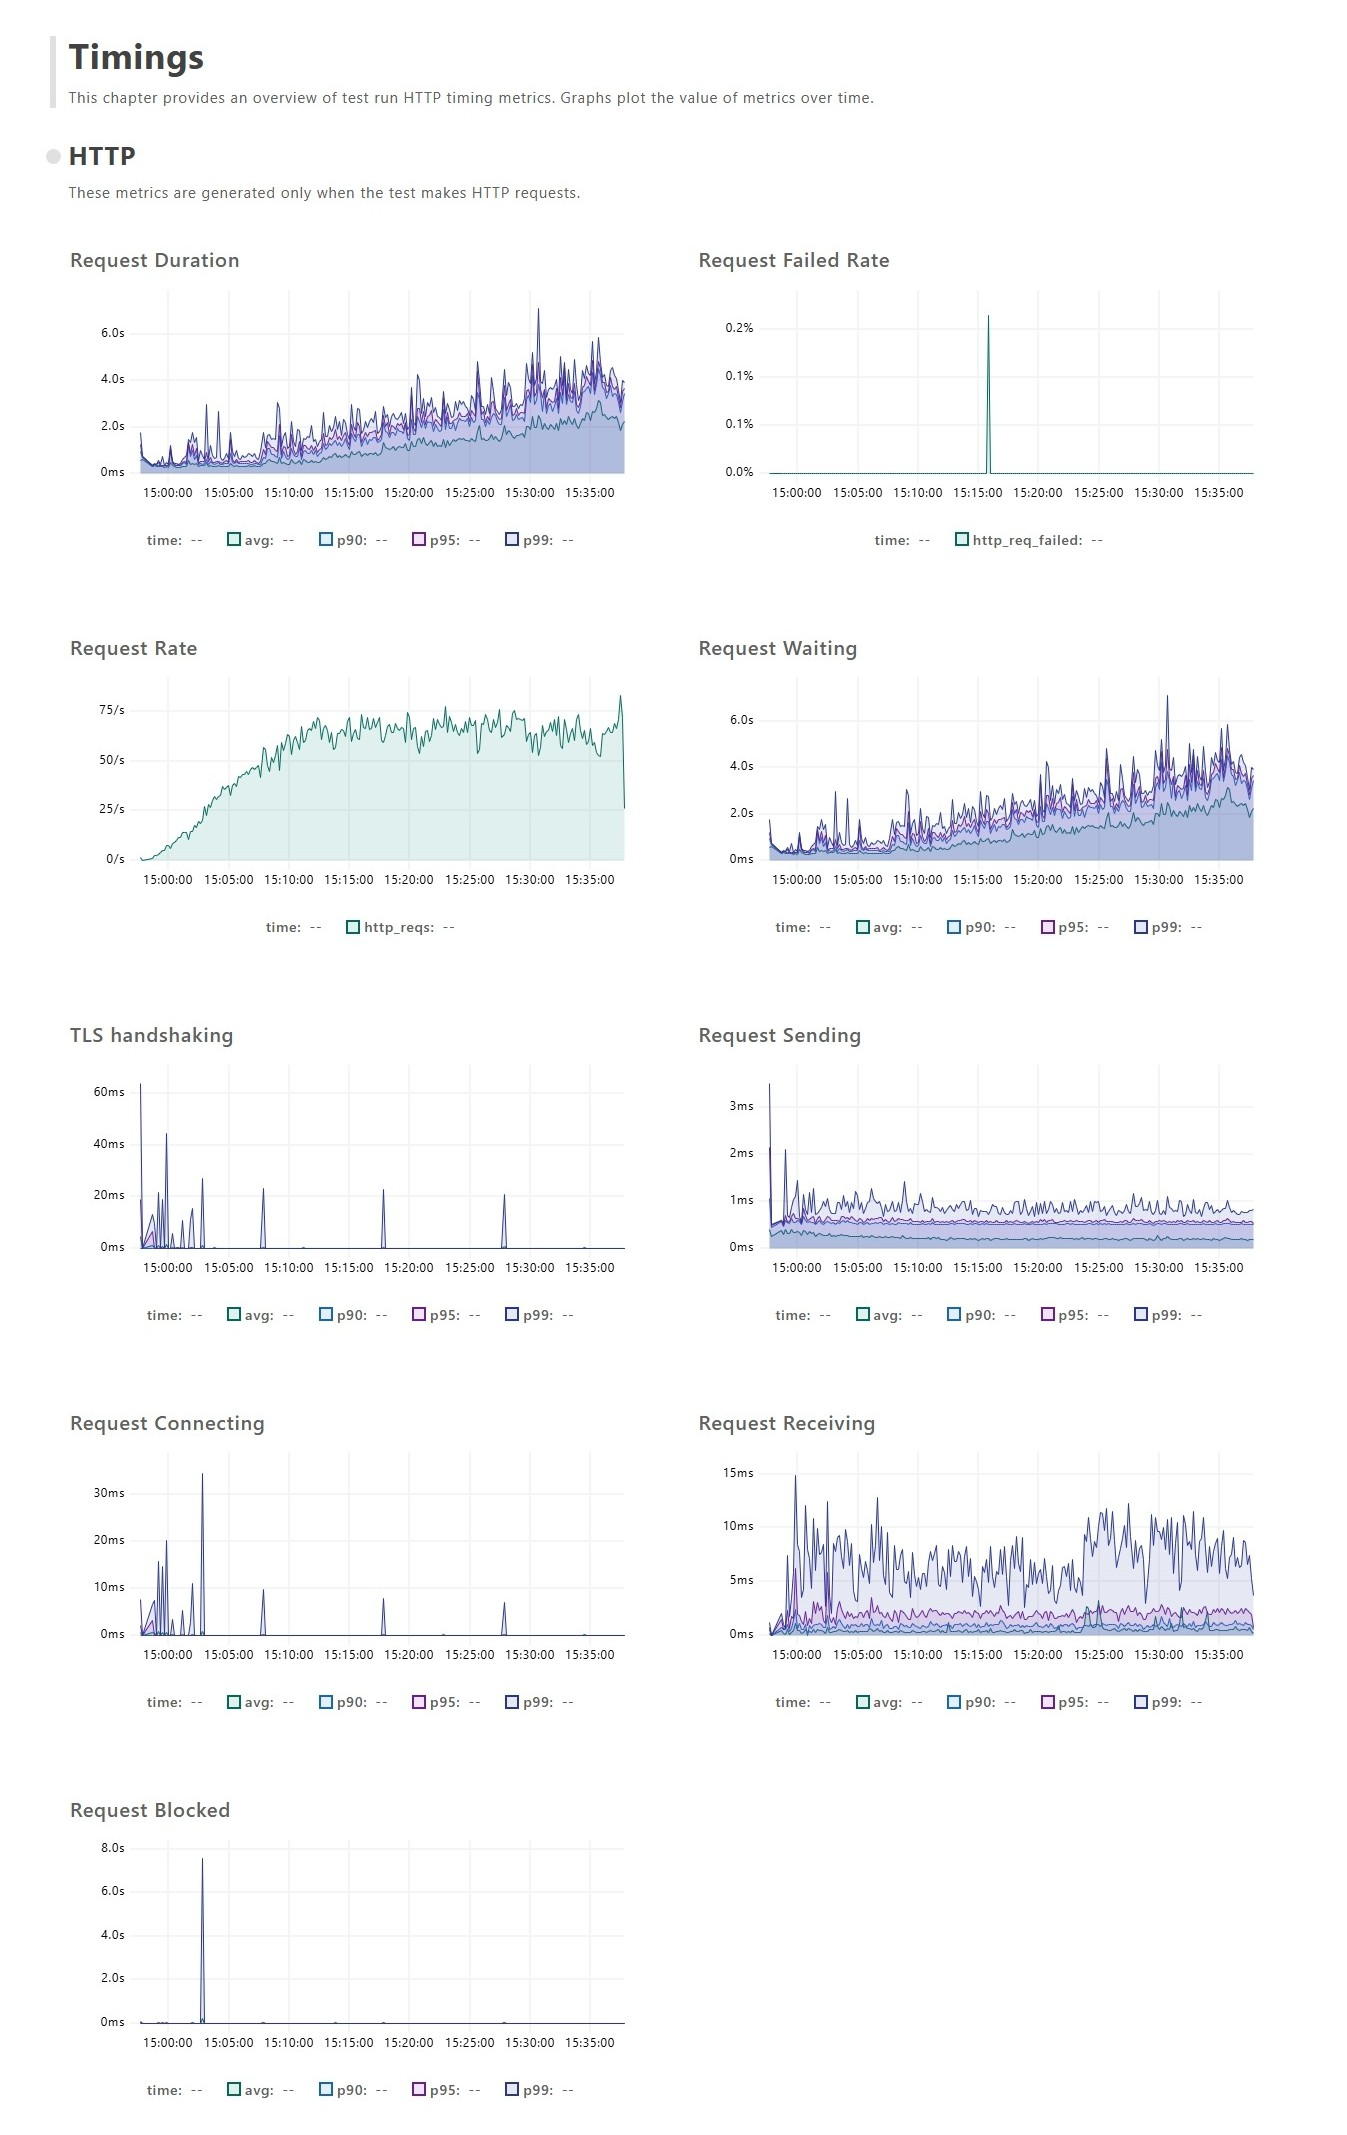
\includegraphics[width=1\textwidth,keepaspectratio]{images/k6-result-timings.jpeg}
\end{figure}

\begin{figure}[H]
      \centering
      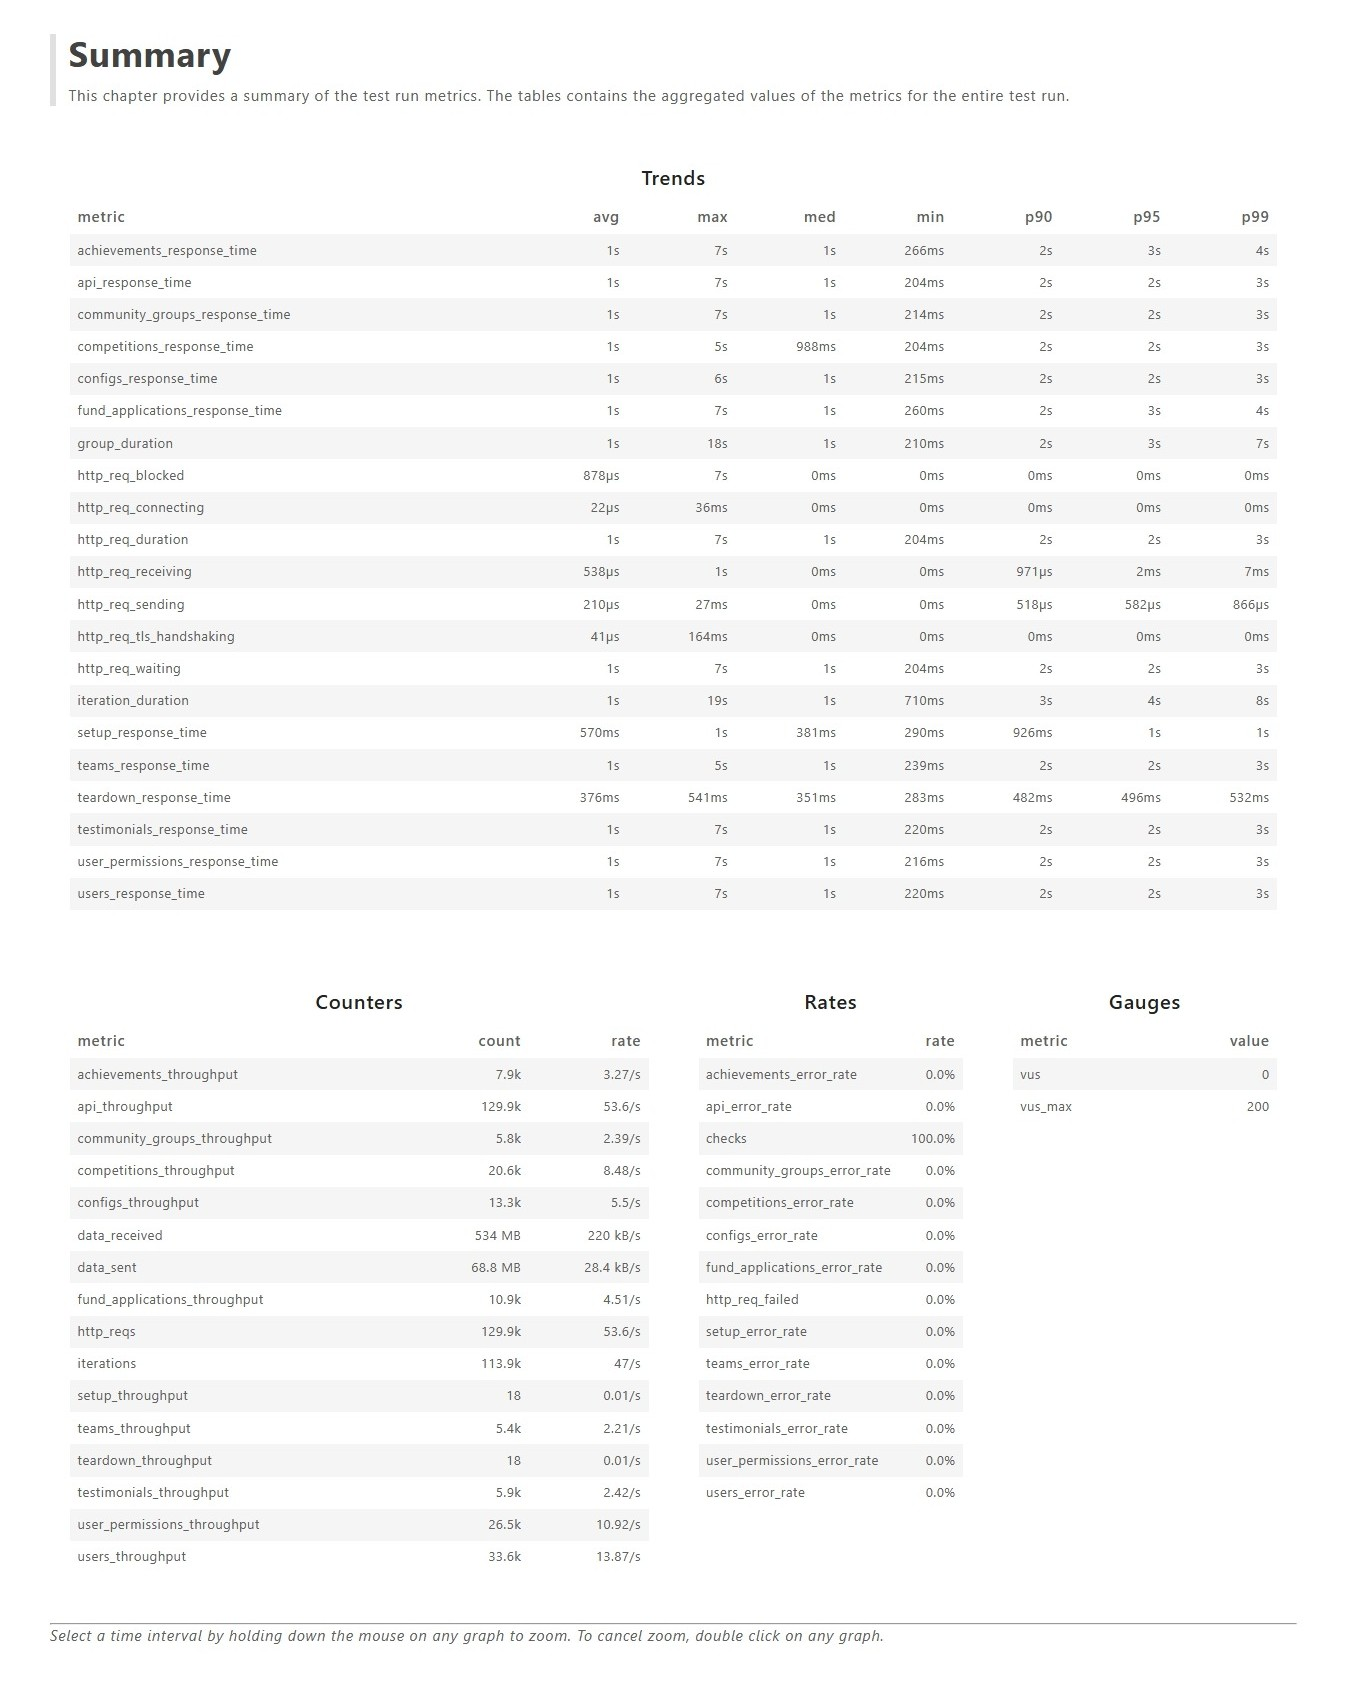
\includegraphics[width=1\textwidth,keepaspectratio]{images/k6-result-summary.jpeg}
\end{figure}
